
\documentclass{article}


%\documentclass[AEJ,reqno]{AEA} % the reqno is no equations numbers on right..

\usepackage{natbib}
\usepackage{graphicx}
\usepackage[figuresright]{rotating}
%\usepackage[abbr]{harvard}
\usepackage{booktabs}  %this is for toprule...
\usepackage{colortbl}
\usepackage{dcolumn}
\usepackage[utf8]{inputenc}
\usepackage{url}
\usepackage{comment}
\usepackage{amsmath}
\usepackage{afterpage}
\usepackage[section]{placeins}
%\usepackage{siunitx}
\usepackage{placeins}
\usepackage{tabu} % for table in markup ds..
\graphicspath{{Figures/}}
%\usepackage{caption} % this is used to add source or additional note on the figures..
\usepackage{subfig}
\usepackage[flushleft]{threeparttable}
\usepackage{physics} % this is used for adding partial derivatives etc..

%\usepackage{showframe}
\usepackage[margin=1.5in]{geometry}

%\usepackage{tablefootnote} % this should be loaded after the hyperref and sideways table packages/environments..


%  http://pdf2docx.com/


%\draftSpacing{1.5}

\begin{document}




\title{Are Improved Homes Overcapitalized in the Long Run?\footnote{Although the research described in this paper has been funded wholly or in part by Corelogic RP Data, it has not been subjected to the Institutes's peer review and therefore may not necessarily reflect the views of the company and no official endorsement should be inferred.}}
%\shortTitle{HOUSING RE-INVESTMENTS AND MARKET VALUE}
\author{Haresh Pardasani, Vito Mollica and Stefan Trueck\thanks{%
Pardasani: Macquarie University, Graduate School of Management; Mollica: Macquarie University, Graduate School of Management; Trueck: Macquarie Unviversity, Department of Business \& Economics. The authors gratefully acknowledge Corelogic RP data and Cordell (a subsidiary of Corelogic) for providing the house price and development approvals data for this research. We would also like to thank Scott Mathews and Kevin Ward for providing valuable feedback during the research.}}
\date{\today}
%\pubMonth{Feb}
%\pubYear{2017}
%\pubVolume{}
%\pubIssue{}
%\JEL{25, 26, 36, 47, 58}
%\Keywords{Housing Re-investment, Home Improvement, Development Approval, House Prices, Real Estate Economics}

\maketitle{}

\begin{abstract}
This paper investigates whether there any returns to home improvements or the returns are simply attributed to market appreciation? Using a fixed effects OLS model on a combined data set of Australian house prices and improvement spending for repeat sale homes with over 55,000 properties, we find that improved homes, in expectations, are overcapitalized. Specifically, the returns on improved homes are, on average, 2.4\% lower than the unimproved homes. This result is consistent to a set of robustness tests. In a further analysis, we also find that, for homeowners who buy and sell in the short run, the improved homes have higher returns than the unimproved homes with the most prominent positive effect seen in extension/alteration of around 5.5\%. This is mainly because homeowners who buy and sell in short run are more likely to have an investment motive right at the beginning and therefore their choices and decision are more guided by making a financial gain. Whereas, the homeowners who buy and sell over longer periods of time, are consuming the housing services and enjoy other social benefits at the cost of lower returns.
\end{abstract}



\section{Introduction}

Amidst rising house prices, housing re-investments in Australia have become an increasingly important instrument for families to meet their growing housing needs. More and more people are turning to home improvements as an alternative to additional housing. Home improvements are defined as activities which increase the stock of housing capital by remodeling the existing home or building a new house without constructing new dwellings. They should be distinguished from maintenance activities that are aimed at offsetting the physical deterioration in housing capital. Examples of home improvements are adding a bedroom or a bathrooms, building a duplex, converting a garage into a room or building a swimming pool. An improvement generally involves major construction activity, whereas maintenance does not.

\begin{figure}[!ht]
\centering
  \subfloat[Total Value of Building Approvals Trend]{%
      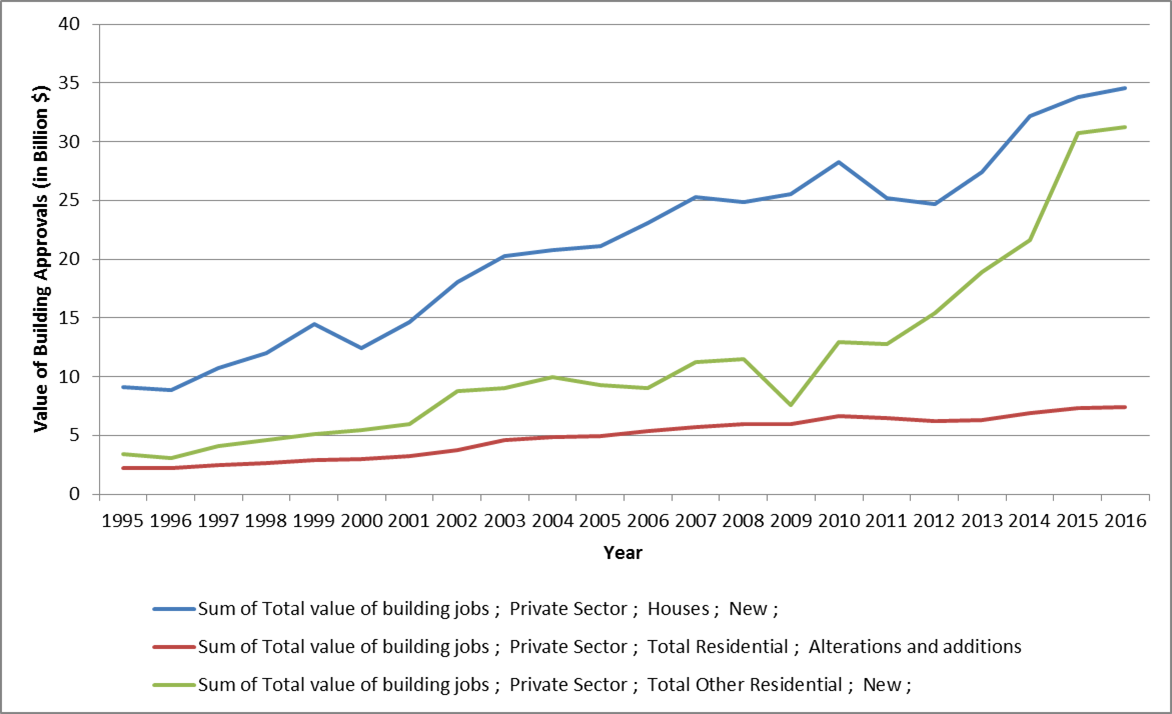
\includegraphics[width=0.75\textwidth]{Figures/Value_building_approvals.png}}\    
  \subfloat[Total Value of Building Approvals]{%
    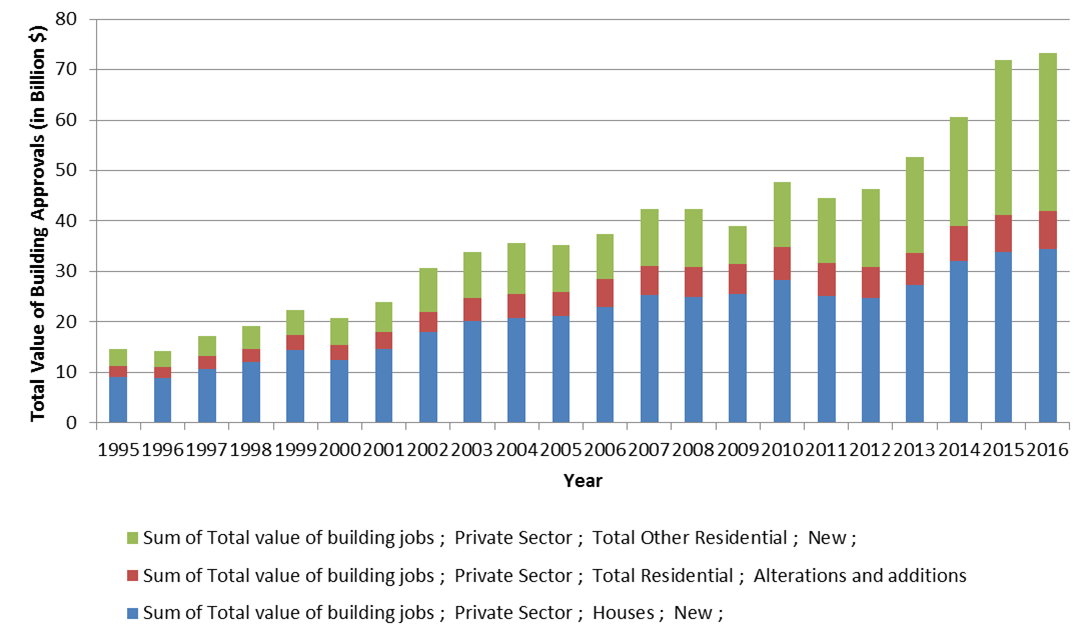
\includegraphics[width=0.75\textwidth]{Figures/ABS_Building_Approvals.png}}\  
 \caption{\small{Panels (A) and (B) show total value of Building Approvals trend and relative percentages}}
\label{fig:Total_Value_of_Building_Approvals}
Source: \scriptsize{Australian Bureau of Statistics}
\end{figure}

Over the last 26 years, home improvement expenditures have increased, both in real terms and as a component of the total residential investment. Investments in 'Houses' constitute close to 70\% of the total residential investments. Around 80\% of those investments come from redeveloping a new houses and remaining 20\% come from alterations and additions to existing houses. \citep{abs1} This however, masks significant variation across different improvement types used in our analysis.

Figure \ref{fig:Total_Value_of_Building_Approvals}, panels (a) and (b), show the total value of granted building approvals in trend and relative percentages. We see that the total value of building approvals for 'New Houses' is constantly growing and is a large component of total residential investment. Building approvals on alterations of existing houses has also increased over the years.

The 'Other residential' category is a building other than houses primarily used for long-term residential purposes and which contains (or has attached to it) more than one dwelling unit for e.g. it includes blocks of flats, home units, attached townhouses, semi-detached houses, duplexes\footnote{Duplexes are considered in the 'Other residential buildings' and Australian Bureau of Statistics does not provide a separate development cost values}. The expenditure on 'other residential' buildings have accelerated in recent years which is evident in the large number of developments of high rise building in the country. In this paper, we focus only on the home improvements for 'Houses' as the building type. 


\begin{comment}

\begin{figure}[!htb]
    \centering
     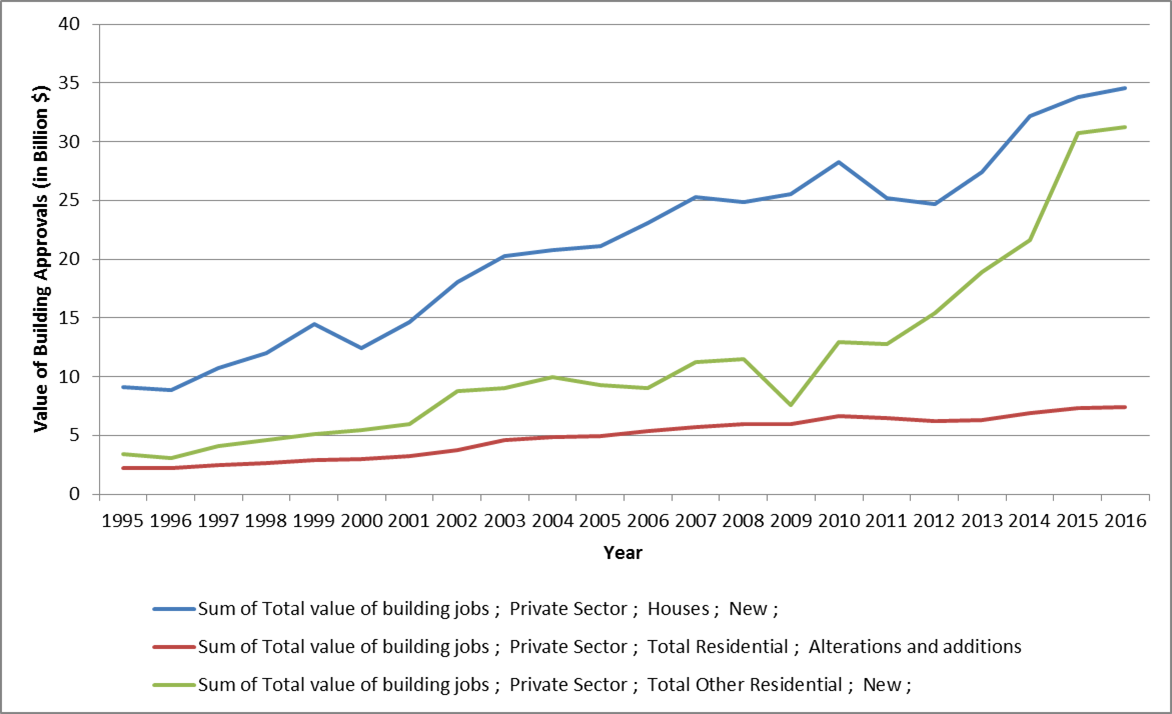
\includegraphics[width=0.75\textwidth]{Figures/Value_building_approvals.png} \par
 \caption{Total Value of Building Approvals Trend}
Source: \scriptsize{Australian Bureau of Statistics}
\end{figure}

\begin{figure}[!htb]
    \centering
    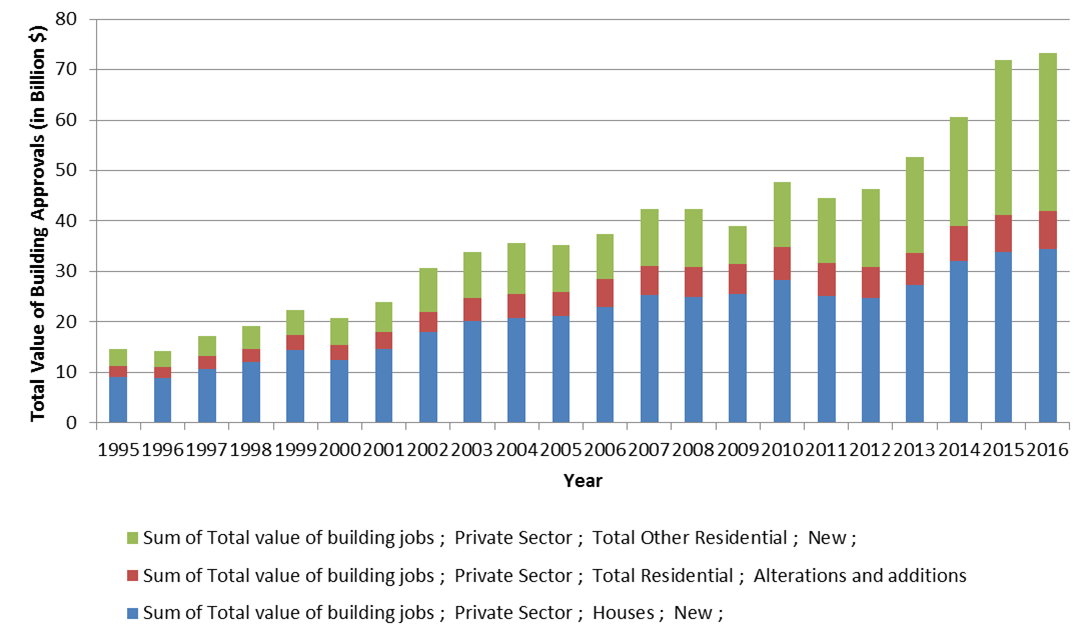
\includegraphics[width=0.75\textwidth]{Figures/ABS_Building_Approvals.png}\par
 \caption{Total Value of Building Approvals}
Source: \scriptsize{Australian Bureau of Statistics}
\end{figure}

\begin{figure}[!htb]
    \centering
    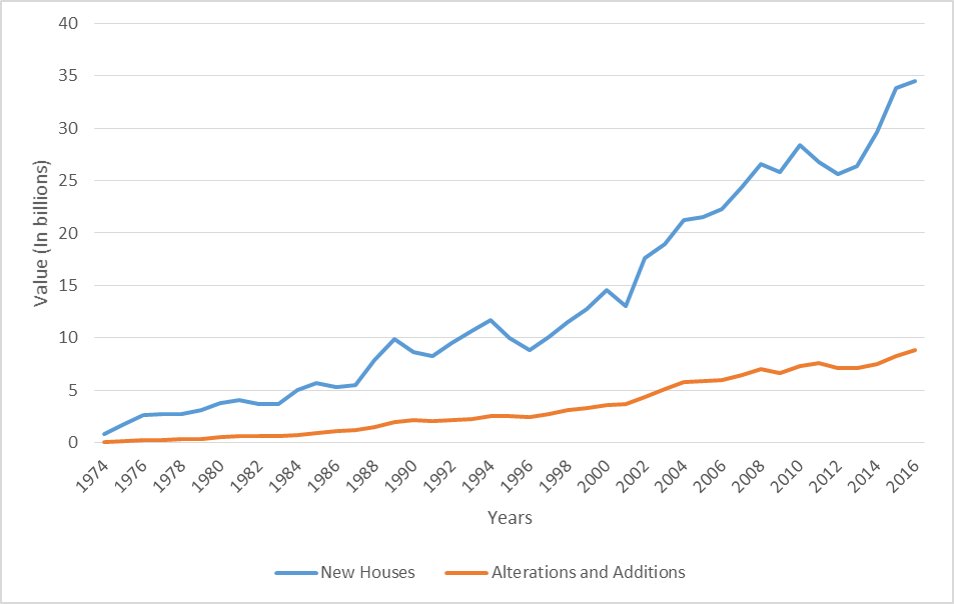
\includegraphics[width=0.75\textwidth]{Figures/value_of_work_done_87520021.png}\par
 \caption{Total Value of Work Done}
 \label{fig:value_of_work_done}
Source: \scriptsize{Australian Bureau of Statistics}
\end{figure}

\end{comment}

With growing spending on home improvements, there is certainly more value created at the macroeconomic level in terms of increased employment, higher production of goods and services. However, from the homeowners perspective, there is a long standing question of the returns from home improvements. Are housing re-investments profitable? Do homeowners who improve their homes make better returns as compared to those who don't? Does the excess value attributed to the home improvement outweigh the costs? Also how do returns compare for homeowners who buy and sell with an investment motive as opposed to people who buy the property for self living? These are some of the questions that we seek to answer.

Looking at development approvals directly, is notoriously difficult given that the improvements for different households occur at different points in time between a repeat sale. Also many household make a development application but never go ahead with the construction and therefore it becomes difficult to estimate the value of home improvement. When people buy an resell the property, they would make a return from the repeat sale. But if homeowners improve their homes in between the repeat sale, they would have also created some value from producing additional housing. The dynamics of both house price appreciation and the home improvement value also add to the challenge.

This paper studies and compares the returns between improved and unimproved homes. We develop a simple fixed effects OLS model in log-returns and compare the means of improved and unimproved homes using a dummy variable and control for the other sources of variations. The results show that when accounted for the development spending, the returns on improved homes, in aggregate, are lower than unimproved homes by around 2.4\%. Although, the degree to which returns are lower vary for different improvement types, we find that all improvement types, except for Duplexes, have lower returns than unimproved homes. These relatively lower returns are not explained by household demographics nor property characteristics, as they are separately controlled for, but rather to the cost of consumption of housing services and other social benefits that are enjoyed. We also find, on the contrary, that homeowners who purchase the property with and investment motive, make higher returns on the home improvement than those who do not improve as compared to people who did not have an investment motive.

The remainder of the paper is organized as follows. In section II we provide a literature review. In section III, we present a simple model of house price return. Section IV describes the data. In section V, we estimate a fixed effects OLS model and compare the returns on improved homes relative to unimproved homes. In section VI, we perform further analysis to examine how returns vary for investor and non-investor groups. In section VII, we discuss the set of robustness tests. Section VIII concludes.


\begin{comment}

The data contains property-specific information for a national-sample of homeowners, including individual house prices, statistical subdivision level Hedonic Index and home improvement expenditures. Using these data, we calculate the expected house price at the time of DA and the home equity of the developed property which is the sum of the expected house price and the cost of home improvement. We then calculate the log return of the property between the resale price and the home equity at the time of home improvement. 



while both fixed effects specifications are estimated on thin samples and accordingly have less statistical power than the main analysis, the estimation results generally confirm the main findings..

 while there is now an abundance of cross-country evidence on the determinants of house price growth, relatively little of this identifies identifies relationship with the housing developments. Papers by..... sos and so...do suggest that the construction costs have effect on the house price returns...so and so...

In our study, we utilise both time and cross-section variation in the developments and house price data. A reasonably long time period of house price data (1990-2016, 26 years) and development data (2000-2016, 16 years) and the

Also the investors are different in their approach, as they may be more astute investors and want to sell for profit. So probably invest in the properties with a point of making money as compared to the others home owners who have families and they are more particular about economic benefit and so they invest wisely. on the other hand, families want to stay in their homes for long term. So they enjoy the non durable housing service as opposed to investors that instead make economic profits.

\end{comment}


\section{Literature Review}

There are several studies that have either modelled the demand for home improvement expenditures as a probability measure or the dollar value and there are other studies that have identified the determinants of home improvement expenditures. However, there is little work done in the literature that attempts to quantify the returns on home improvement.

\citet{boehm1986improvement} studies the determinants of home improvement expenditures using a data sample created from surveys. The author relates the home improvement expenditure to the consumption benefits and to the resale value. More specifically, the author suggests that the marginal benefit function represents the present value of the consumption benefits derived from additional unit of home improvement and the present value of change in resale value resulting from improvement which is the investment return on home improvements. However they do not estimate the return on the home improvement.

Also \citet{boehm1986improvement} states that the investment return to home improvements depends on the price of housing services expected to prevail at the time the house is sold. However they do not estimate the relationship between investment return and the home improvement. The state that this price is positive function of the current neighbourhood price of services and expected rate of house price appreciation and therefore uses other neighbourhood quality variables such as crime rate in the area, quality of schools, roads, sidewalks etc as explanatory variables in the empirical regression. \citet{galster1987homeowners} studies the determinants of housing reinvestment expenditures in a choice framework of improving compared to do nothing option. However they also do not estimate the returns for improved and unimproved homes.

\citet{mendelsohn1977empirical} builds a theoretical model on home improvements and relate relates the amount of self labour invested in the home improvement as opposed to hired labour. The author suggests that homeowners work on their house until the rewards from that work are equal to the value of his leisure time. The reward of his work depends on his productivity, the market price of housing and the marginal utility of both housing and assets. The author also suggests that the marginal value of a dollar spent on housing improvements, assets or other goods should all be the same. \citet{potepan1989interest} focus on the consumption demand of home improvement i.e. the home improvement demand for owner occupier. They argue that home owners face choice between improving their existing housing and moving to obtain additional housing. They model the demand for housing reinvestment using interest rates and incomes and show that the housing investment is positively related to the interest rates as interest rates are high people are less likely to move and therefore reinvest in their own homes. Also housing reinvestment is negatively related to the incomes as higher income would make them more like to move instead of reinvesting in their homes. \citet{montgomery1992explaining} models the housing improvement demand by simultaneously allowing for the home owners to choose the level of stock they hold and the means by which they adjust their current holdings of the housing stock, i.e. either moving to a new home, or improving the existing home or doing nothing. 

\citet{gyourko2003urban} describes the role of construction costs in housing decline in America. Their main question in this paper is to study the sensitivity of investment to construction cost. They suggest that a rational investor would not invest in the housing if the home values are below replacement cost. There is often decay in the housing markets of declining areas. In their paper, they ask whether this process is endogenously demand driven or whether the supply side of the housing market plays some role. They find that housing prices are close to replacement cost in most areas. For houses in specific neighbourhoods where the house prices are near construction costs, modest difference in replacement cost may be critical on the margin to determining whether a fundamental decay sets in or reinvestment occurs in the face of a negative demand shock. They say that the construction costs need not be exogenous to the decay process i.e. the construction costs may cause decay process which in turn may increase the construction cost and further induce the decay process. They suggest that if the construction cost were flexible downward in response to the negative demand shocks, then there need not even be a negative impact on housing investment. Their analysis finds that the construction costs are not very sensitive to construction levels. there is a substantial between city variation in the costs that cannot be account for with a standard, upward sloping supply schedule. The authors also note that owner occupiers may reinvest for non financial reasons as they are the consumers of the housing stock. 


\citet{gyourko2004reinvestment} finds that demand for renovation services to be relatively price-inelastic. They also report that there is a substantial heterogeneity in the distribution of home values across different market areas. In places with high house value. a 1-percent drop in the construction cost would not change the fraction of homes with value above replacement costs. Land prices are so high in these areas that there are virtually no homes valued at less than 110 percent of the construction costs. They also confirmed that the relationship between renovation and home values is strongly linear. They confirmed this by introducing 20 dummies for each corresponding value quantile into regressions and they still could reject at the 5 or 10 percent levels. \citet{guthrie2010house} suggests that the new house prices are considerably above the direct construction costs. This premium can be attributed to the option value of delaying the development of marginal piece of land. Competition can reduce the this option value but as long as there is heterogeneity in the land, the value cannot be reduced to zero. In the US data they find that this premium is economically significant.

All these authors have explained the factors and how they affect the home improvement demand and the expenditures. However, there is no study that estimates the returns to home improvements. \citet{simons2009housing} quantifies the returns on the government spending in the context of community housing. Also, unlike our method that uses a regression model and controls for the other factors, they use a cost benefit analysis framework and show that every dollar invested by local government returns \$0.55 on average. Their underlying idea is that the return or benefit is a derived measure which is a function of one time property tax and regular tax income earned by the government and also the loan and the interest payments made by homeowners.

In the next section, we develop a simple model of house price returns.


\section{A Model of House Price Return}

Let $t$ represent a point in time. Let subscript $-1$ represent time of purchase, $+1$ be the time of subsequent sale post DA (resale) and for improved homes, $0$ represent time of home improvement\footnote{For purpose of model exposition, we assume the time of DA activity as a point in time, however, the point actually represents an interval from approval date till the completion of improvement. The point in time when improvement is completed is equal to the time of building approval plus expected commencement time (c) and plus average construction time (c'). In the empirical analysis, we adjust for this interval accordingly}. Therefore, $$t_{-1} < t_0 < t_{+1}$$ Also let time between $t = -1$ and $t = 0$ be given by $t_{0} - t_{-1} = t_1$ and the time between $t = 0$ and $t = {+1}$ be given by, $ t_{+1} - t_{0} = t_2$.


We consider that the value of a house comprises of three components, namely, Land value ($L$), non-durable consumption (B) (i.e. the value of the building) and durable consumption (H) (i.e. the value of housing service) \citep{flavin2008model}. Let $R$ be the the composite rent to be paid for the collective value of the house at a given time t. Then, using the model given by \citet{kiel1995effect}, the house value $V$ at time $t$ can be modelled as,

\begin{equation}
    V(t) = \int_{T}^{\infty} R e^{\alpha t} e^{-bt} e^{ht} e^{\sum_{i} \mu_i K_i} e^{-rt} dt
\end{equation}

where, $R$ is the composite rent at some initial time t, $\alpha$ is the appreciation rate of the land, $b$ is the depreciation rate for the non-durable consumption (building value), $h$ is the appreciation rate, if any, for the durable consumption (housing service), $K_i$ is the set of control variables where $i$ indexes different control factors, $\mu_i$ is the corresponding effect of the controls on the house prices and $r$ is the discount rate. 

The houses in Australia could be on a freehold or leasehold land title. In freehold lease the homeowner has full ownership of the property until perpetuity while in leasehold, homeowner can possess the property for up to 99 years. Most of the residential properties in Australia are freehold. Therefore the rents to be paid for periods far out in the future would be negligible. Hence the integral of the above equation will be finite. 

Solving the above integral yields,

\begin{equation}
    V(t) = \frac{R e^{-(r-\alpha+b-h)T} e^{\sum_{i} \mu_i K_i}}{r-\alpha+b-h}
\end{equation}

Now, for repeat sales data, we have sales prices observed twice within a specified period. Using equation 2, we can calculate the value of the house at the time of purchase as,

\begin{equation}
    V_{-1} = \frac{R_{-1} e^{-(r-\alpha+b-h)T} e^{\sum_{i} \mu_i K_i}}{r-\alpha+b-h}
\end{equation}

Similarly, the value of the house at the time of resale can be given as,

\begin{equation}
    V_{+1} = \frac{R_{+1} e^{-(r-\alpha+b-h)(T+t_{+1}-t_{-1}} e^{\sum_{i} \mu_i K_i}}{r-\alpha+b-h}
\end{equation}

Now, we can calculate the appreciation rates in terms of log-returns as,

\begin{equation} \label{eq:a}
    ln [V_{+1}/V_{-1}] = ln [ (\frac{R_{+1} e^{-(r-\alpha+b-h)(T+t_{+1}-t_{-1})} e^{\sum_{i} \mu_i K_i}}{r-\alpha+b-h}) / (\frac{R_{-1} e^{-(r-\alpha+b-h)T} e^{\sum_{i} \mu_i K_i}}{r-\alpha+b-h})]
\end{equation}
Simplifying equation \ref{eq:a} and re-arranging gives,
\begin{equation}
    ln [V_{+1}/V_{-1}] = ln [R_{+1}/R_{-1}] + (\alpha-b+h-r)(t_{+1}-t_{-1}) 
\end{equation}

This model is estimated using the log returns of repeat sales prices of houses over time. Since, the changes in the supply and demand of houses have been found to affect appreciation rates, these characteristics are included in the regressions (although the equations suggests that these cancel out). The composite rate $(\alpha+h-r-b)$ between the sales are inseparable but jointly observed in the market index. Also, although the depreciation rate is captured in the Market index, we explicitly allow for the depreciation rate to be included in the regression to capture the effect of depreciation for improved homes\footnote{The hedonic house price index developed by CoreLogic does not account for the age of the property and therefore the effects of depreciation may not have been captured entirely. In our model, we explicitly include the age of the DA and control for linear as well as any quadratic effects of depreciation}. The equation 6, therefore, is estimated as,

\begin{equation} \label{eq:estimate}
    ln [V_{r}/V_{p}] = a_0 + \beta{(Market Return)} - d(t2-t1) + \sum_{i}\mu_i K_i )
\end{equation}

where $a_0 = ln [R_{+1}/R_{-1}]$ is a constant and $\beta$ is a composite rate of return equal to $(\alpha+h-r-b)$ attributed to the average market appreciation.


\section{Institutional Setting and Data}

Our paper focuses on the residential re-investments in building types - 'Houses' only that are single family detached homes. Other residential building types such as units/apartment, townhouses and semi-detached houses are a small portion of improvement spending and therefore not included in the analysis. The improvement activity can have several elements such as completely demolishing and rebuilding a new house from scratch or adding a bedroom, bathroom or carport, or putting a veranda or pergola. These elements of home improvements are grouped into different improvement types such as 'houses'/'single dwelling', 'extensions/alterations', 'carports/garages/sheds', 'swimming pools', 'verandas/pergolas' and 'duplexes'.

For Duplexes, households typically split the land into two lots of equal sizes and build two duplexes on the land and then sell one of the duplexes. The price of previous sale is the price at which the owner buys the whole lot which is subdivided into two, but when they sell after building a duplex, the price recorded in the house price data set is only for one of the duplexes. Therefore, to account for this land-split and the double equity that is generated for homeowners, we assume that the other lot also sells at the same price and therefore we double the resale price in our analysis. 

Prior to carrying out any home improvement activity, homeowners are required to obtain a building permit/development approvals from their local councils. To do that, homeowners need to lodge a formal development application (DA) to their local councils detailing the plan and the cost of developments which is estimated by their builders. As part of the development approval applications, information on development cost and the type of developments are collected and we use this reported development cost as a expected value for the actual home improvement expenditures\footnote{As the DA fees charged by the local councils are typically a percentage of the home improvement expenditure, the households have incentive to declare lower costs so that they will have to pay lower fees. Therefore the DA costs recorded in the DA data set may be slight underestimates of actual home improvement expenditures.}. 

Homeowners can choose to carry out multiple improvements at the same time, For example, add a bedroom and also construct a swimming pool. In such cases homeowners can submit their plan for multiple improvements in the same development application. In our data set, even if there is one development application, multiple improvements are recorded as separate records. If homeowner carries out multiple types of improvements at different times, then obviously, they have to make multiple applications. Once the application is received, the council reviews the development plan and if it satisfies the requirements, the development approval is granted to the homeowners. This is the date when building approval is received that we use in our model as the date of improvement.

The value of additional housing acquired through home improvement is unobserved until the property is sold. When the property is sold the value of additional housing will be implicit in the sale price. Therefore in our analysis we consider only the repeat sales records with a development work carried out between those repeat sales. 

We use a unique data set of repeat sales created by combining the development approvals\footnote{Development Approval's data is provided by Cordell and collected through the surveys of local councils.} and the house price data\footnote{House price data is provided by CoreLogic RP data and collected from real estate agents, banks and local government bodies. The house prices are recorded in CoreLogic's database only when the property is either listed, sold, valued or financed.}. The house price data and the development approvals data are available from 1990 to 2016 and from 2004 till 2016 respectively. The combination of these data-sets are well suited for this study because together they provide detailed information on individual house's sale price and improvement spending over time, date of building approvals and classification of home improvement types. This allows us to estimate returns on different types of home improvements. Finally from the house price data, we calculate returns for a control sample of unimproved homes. This enables identification on whether the returns for homes with improvement are worse than the 'do-nothing option'.
            
After filtering the data for, irrelevant sales types\footnote{Sales where transfers are of the types 'gift', 'court order', 'family sale', 'extraordinary circumstances', 'mortgage in possession', 'part-sale/consideration represents partial interest in the property', 'rebated-sale/negotiated sale', 'residential-redevelopment', transfer by death or transfer by bankruptcy. These types of sale represented ~3.5\% of the total population data set.}, duplicates\footnote{These represent cases where the entire record was duplicated or cases where some of the columns are duplicates but others were different - for example, all other columns had same entries but the construction type was mentioned either in the full form as 'alterations/additions' or in abbreviated form  as 'alts/addns' or was misspelled during data entry. In these cases, we took only one of the records. There were cases, where all the columns were same, but there were differences in dates. In this case, we took the record with the latest date as that it was highly unlikely for households to carry out same type of construction twice and so took the latest DA record.}, invalid\footnote{These were the cases where the homeowners submit a revised application after the approval due to change in their development plans and therefore the previous development approval becomes invalid} and bad records\footnote{These are reporting or coding errors. For example, the reported value may have a missing zero (a \$50,000 home recorded as a \$5000 home) or reported in thousands or dollars (a \$50,000 home recorded as \$50 home). With no systematic way of identifying and correcting for these cases, we exclude the outliers at bottom 1 percentile and 99.9 percentile}, we have roughly 5.4m total homes with repeat sales and among those 1.6m houses have development approvals in Australia. On combining these two data sets, we have a unique sample of 259,428 improved homes that have repeat sales and improvement carried out between the repeat sales. 

However, of these 259,428 records, there could be some properties that received development approvals but haven't gone ahead with their development. Based on the available data, there is no definitive way to identify all the properties that have actually completed their development. It is important to distinguish between properties that have obtained building approvals but haven't gone ahead with the construction and those that have, since, if the property has not gone ahead with their development then we would have accounted for the improvement cost, however, the value of that improvement would be implicitly excluded from the contract price and therefore we would underestimate the returns and cause a downward bias.

Therefore we need to identify a robust set of properties where development work has been completed. To do so, we compare the attributes at the time of resale to the previous sale and include only those properties, where one of the attributes (i.e. bedrooms, bathrooms or car spaces) has increased from the time of previous sale, for duplexes, new house and extension/alterations\footnote{Attribute changes for verandas and pergolas were not confirmed as those attribute flags are not available. We assume that, considering relatively smaller outlay, households would have gone ahead with the construction.}. For swimming pools, we confirmed if the swimming pool flag equals 'true' at the time of current sale. 


% Table generated by Excel2LaTeX from sheet 'Sheet7'
\begin{table}[t!p]
  \centering
  \caption{Distribution by DA Type and State}  \label{tab:distribution}%
  \resizebox{\textwidth}{!}{
  \begin{threeparttable}
    \begin{tabular}{lccccccccc}
    \toprule
          & \multicolumn{9}{c}{State} \\
\cmidrule{2-10}          & ACT   & NSW   & NT    & QLD   & SA    & TAS   & VIC   & WA    & Total \\
    \midrule
    Non-DA & 13,421 & 245,948 & 12,707 & 319,273 & 77,504 & 35,803 & 255,412 & 129,746 & 1,089,814 \\
    Carports/Garages/Sheds &       & 301   &       & 307   & 98    & 23    & 194   & 149   & 1,072 \\
    Duplex &       & 612   &       &       & 1     &       & 122   &       & 735 \\
    Extension/Alteration &       & 4,616 &       & 681   & 726   & 74    & 3,412 & 1,208 & 10,717 \\
    House/Single Dwelling &       & 1,450 &       & 584   & 514   & 15    & 2,676 & 783   & 6,022 \\
    Multiple DA &       & 1,239 &       & 1,194 & 763   & 10    & 1,528 & 4,324 & 9,058 \\
    Swimming Pool &       & 3,891 &       & 3,626 & 1,200 & 8     & 2,640 & 4,966 & 16,331 \\
    Verandahs \& Pergolas &       & 1,072 &       & 1,976 & 1,702 & 103   & 2,746 & 4,199 & 11,798 \\
    Total & 13,421 & 259,129 & 12,707 & 327,641 & 82,508 & 36,036 & 268,730 & 145,375 & 1,145,547 \\
    \bottomrule \\ [-2ex] 
\end{tabular}%
  \begin{tablenotes}[para,flushleft]
  \LARGE
      The table shows the distribution of DAs by type and state. We see that there are a total of around 1.08m unimproved homes. For improved homes, the highest number of DAs in our sample are of the type Swimming Pools - 16,331, followed by Verandas/Pergolas - 11,798 and Extension/Alterations - 10,717. The least number of DAs in our sample are for Duplexes - 735 and Carport/garages/sheds - 1,072. Across states, we have highest number of DAs in VIC - 13,196 followed by NSW -13,181. ACT and NT do not have any observations for DAs.
\end{tablenotes}    

    \end{threeparttable}
    }

  \bigskip

  \caption{Summary Statistics - DA Cost (Constant Dollar 2016-Q3)} \label{tab:DA_cost_statistics_rs_const_dollar}%
   \resizebox{\textwidth}{!}{
    \begin{threeparttable}
    \begin{tabular}{rccccccc}
    \toprule
          & \multicolumn{7}{c}{Mean} \\
          & \multicolumn{7}{c}{(Std. deviation)} \\
\cmidrule{2-8}    \multicolumn{1}{c}{DA Type} & \multicolumn{1}{c}{NSW} & \multicolumn{1}{c}{QLD} & \multicolumn{1}{c}{SA} & \multicolumn{1}{c}{TAS} & \multicolumn{1}{c}{VIC} & \multicolumn{1}{c}{WA} & \multicolumn{1}{c}{All States} \\
    \midrule
    \multicolumn{1}{l}{Carports/Garages/Sheds} & 17,136 & 14,935 & 11,061 & 15,296 & 14,279 & 14,586 & 15,039 \\
          & (12,799) & (10,527) & (6,329) & (8,745) & (12,468) & (8,717) & (11,139) \\
    \multicolumn{1}{l}{Duplex} & 491,765 &       & 172,374 &       & 760,411 &       & 535,922 \\
          & (233,881) &       & NA    &       & (278,275) &       & (261,690) \\
    \multicolumn{1}{l}{Extension/Alteration} & 107,353 & 65,979 & 85,077 & 82,035 & 138,539 & 129,736 & 115,492 \\
          & (106,108) & (74,837) & (69,411) & (84,990) & (143,566) & (140,012) & (121,634) \\
    \multicolumn{1}{l}{House/Single Dwelling} & 295,850 & 288,558 & 240,484 & 239,705 & 377,409 & 389,903 & 338,749 \\
          & (188,719) & (115,932) & (128,832) & (128,905) & (282,821) & (285,465) & (244,922) \\
    \multicolumn{1}{l}{Multiple DA} & 282,546 & 251,220 & 208,279 & 153,836 & 375,217 & 274,928 & 284,015 \\
          & (272,418) & (217,374) & (146,280) & (104,467) & (297,933) & (229,289) & (245,612) \\
    \multicolumn{1}{l}{Swimming Pool} & 27,846 & 29,349 & 27,320 & 38,776 & 40,657 & 24,360 & 29,157 \\
          & (16,029) & (13,238) & (18,725) & (36,661) & (32,755) & (100,236) & (58,170) \\
    \multicolumn{1}{l}{Verandas/Pergolas} & 20,188 & 15,309 & 12,810 & 18,859 & 16,507 & 10,907 & 14,135 \\
          & (15,041) & (12,909) & (8,954) & (22,191) & (14,186) & (8,018) & (11,958) \\
    \multicolumn{1}{l}{All DA Types} & 129,786 & 78,234 & 79,963 & 59,266 & 173,012 & 116,434 & 123,863 \\
          & (182,441) & (133,177) & (115,008) & (86,891) & (240,681) & (199,600) & (194,603) \\
    \bottomrule \\ [-2ex] 
    \end{tabular}%
   
   \begin{tablenotes}[para,flushleft]
  \LARGE
     This table shows improvement spending by type and state reported in constant dollar of 2016-Q3. We see that Duplex has the highest average cost of development of \$535,922 followed by House/Single Dwelling with average cost of \$338,749. Developing a House/Single Dwelling is most expensive in Western Australia. This is because the houses in Western Australia are bigger and also remote which adds to increased transportation costs. Verandas/Pergolas have the least average cost of \$14,135 and then followed by Carports/Garages/Sheds with average cost of around \$15,039. Swimming Pools in Victoria are most expensive to built with average cost of \$40,657 due to the heating systems in Victorian pools. Across states, we see that the highest improvement spending is done in Victoria with average spending of \$173,012 followed by NSW with average spending of \$129,786.
\end{tablenotes}   
    
 \end{threeparttable}  
    
    }%
    

\end{table}%

\vspace*{-\baselineskip}
% Table generated by Excel2LaTeX from sheet 'Sheet7'
\begin{table}[!t]
  \centering
  \caption{Summary Statistics - DA Cost (Constant Dollar 2016-Q3)}
    \resizebox{\textwidth}{!}{
    \begin{tabular}{rccccccc}
    \toprule
          & \multicolumn{7}{c}{Mean} \\
          & \multicolumn{7}{c}{(Std. deviation)} \\
\cmidrule{2-8}    \multicolumn{1}{l}{DA Type} & \multicolumn{1}{l}{NSW} & \multicolumn{1}{l}{QLD} & \multicolumn{1}{l}{SA} & \multicolumn{1}{l}{TAS} & \multicolumn{1}{l}{VIC} & \multicolumn{1}{l}{WA} & \multicolumn{1}{l}{All States} \\
    \midrule
    \multicolumn{1}{l}{Carports/Garages/Sheds} & 17,136 & 14,935 & 11,061 & 15,296 & 14,279 & 14,586 & 15,039 \\
          & (12,799) & (10,527) & (6,329) & (8,745) & (12,468) & (8,717) & (11,139) \\
    \multicolumn{1}{l}{Duplex} & 491,765 &       & 172,374 &       & 760,411 &       & 535,922 \\
          & (233,881) &       & NA    &       & (278,275) &       & (261,690) \\
    \multicolumn{1}{l}{Extension/Alteration} & 107,353 & 65,979 & 85,077 & 82,035 & 138,539 & 129,736 & 115,492 \\
          & (106,108) & (74,837) & (69,411) & (84,990) & (143,566) & (140,012) & (121,634) \\
    \multicolumn{1}{l}{House/Single Dwelling} & 295,850 & 288,558 & 240,484 & 239,705 & 377,409 & 389,903 & 338,749 \\
          & (188,719) & (115,932) & (128,832) & (128,905) & (282,821) & (285,465) & (244,922) \\
    \multicolumn{1}{l}{Multiple DA} & 282,546 & 251,220 & 208,279 & 153,836 & 375,217 & 274,928 & 284,015 \\
          & (272,418) & (217,374) & (146,280) & (104,467) & (297,933) & (229,289) & (245,612) \\
    \multicolumn{1}{l}{Swimming Pool} & 27,846 & 29,349 & 27,320 & 38,776 & 40,657 & 24,360 & 29,157 \\
          & (16,029) & (13,238) & (18,725) & (36,661) & (32,755) & (100,236) & (58,170) \\
    \multicolumn{1}{l}{Verandahs/Pergolas} & 20,188 & 15,309 & 12,810 & 18,859 & 16,507 & 10,907 & 14,135 \\
          & (15,041) & (12,909) & (8,954) & (22,191) & (14,186) & (8,018) & (11,958) \\
    \multicolumn{1}{l}{All DA Types} & 129,786 & 78,234 & 79,963 & 59,266 & 173,012 & 116,434 & 123,863 \\
          & (182,441) & (133,177) & (115,008) & (86,891) & (240,681) & (199,600) & (194,603) \\
    \bottomrule
    \end{tabular}%
    }
  \label{tab:DA_cost_statistics_rs_const_dollar}%
\end{table}%


Properties where the previous attributes were missing or the attributes remained unchanged or decreased were excluded from the analysis. We further excluded records where one of the sale transaction, either purchase or a resale, is a land transaction. So finally we have a robust sample of 55,789 records for our analysis. 

Since the development approvals data is available from 2004, we cannot ascertain that the homes in control sample have not carried out any improvement prior 2004 and this could lead to biased results. Therefore, from our control sample, we exclude all the homes where purchases are prior 2004. Also, although, the argument applies to improved homes as well, but in the interest of having reasonable sample size and since there is no bias created as improvement cost will be underestimated and therefore does not affect the result adversely\footnote{We also perform analysis excluding the purchase prior 2004 for improved homes in the robustness section}, we use the full sample of improved homes.

Table \ref{tab:distribution} and \ref{tab:DA_cost_statistics_rs_const_dollar} show the distribution and descriptive statistics of DAs by type and state at repeat sale level. We see that on average the highest cost is for a Duplex \$535,922 with standard deviation of \$261,690 followed by House/Single Dwelling of around \$338,749 an standard deviation of \$244,922. Also the highest cost across states, is for Victoria of \$173,012 followed by New South Wales of \$129,786. 

%% Table generated by Excel2LaTeX from sheet 'Count Distribution'
\begin{table}[h]
  \centering
  \caption{Distribution of DAs by type and state (Individual DAs)}
 \resizebox{\columnwidth}{!}{
    \begin{tabular}{lrrrrrrr}
    \toprule
          & \multicolumn{7}{c}{State} \\
\cmidrule{2-8}    DA Type & \multicolumn{1}{c}{NSW} & \multicolumn{1}{c}{QLD} & \multicolumn{1}{c}{SA} & \multicolumn{1}{c}{TAS} & \multicolumn{1}{c}{VIC} & \multicolumn{1}{c}{WA} & \multicolumn{1}{c}{Total} \\
    \midrule
    Duplex &               663  &             -    &                 1  &              -    &               137  &                   -    &                 801  \\
    Extension \& Alteration &           5,355  &         945  &             928  &             78  &           3,884  &            1,763  &            12,953  \\
    Garages/Sheds \& Carports &               392  &         395  &             139  &             24  &               239  &                223  &              1,412  \\
    House/Single Dwelling &           2,040  &      1,346  &          1,017  &             20  &           3,723  &            4,127  &            12,273  \\
    Swimming Pool &           5,031  &      4,699  &          1,644  &             11  &           3,715  &            8,175  &            23,275  \\
    Verandahs \& Pergolas &           1,289  &      2,447  &          2,188  &           117  &           3,390  &            6,198  &            15,629  \\
    Total &         14,770  &      9,832  &          5,917  &           250  &         15,088  &          20,486  &            66,343  \\
    \bottomrule
    \end{tabular}%
    }
  \label{tab:dist_da_state_type}%
\end{table}%

%% Table generated by Excel2LaTeX from sheet 'Count Distribution'
\begin{table}[!ht]
  \centering
  \caption{Distribution of DAs by type and state (Between Repeat Sales)}
  \resizebox{\columnwidth}{!}{
    \begin{tabular}{lrrrrrrr}
    \toprule
          & \multicolumn{7}{c}{State} \\
\cmidrule{2-8}    DA Type & \multicolumn{1}{c}{NSW} & \multicolumn{1}{c}{QLD} & \multicolumn{1}{c}{SA} & \multicolumn{1}{c}{TAS} & \multicolumn{1}{c}{VIC} & \multicolumn{1}{c}{WA} & \multicolumn{1}{c}{Total} \\
    \midrule
    Duplex &               613  &       &                 1  &       &               122  &       &                 736  \\
    Extension/Alteration &           4,669  &           681  &             727  &             74  &           3,437  &            1,221  &            10,809  \\
    Garages/Sheds \& Carports &               302  &           307  &               98  &             23  &               194  &                151  &              1,075  \\
    House/Single Dwelling &           1,479  &           590  &             516  &             15  &           2,686  &                792  &              6,078  \\
    Swimming Pool &           4,007  &        3,701  &          1,248  &               9  &           2,703  &            5,052  &            16,720  \\
    Verandahs \& Pergolas &           1,097  &        2,053  &          1,737  &           109  &           2,795  &            4,274  &            12,065  \\
    Multiple DAs between repeat sale &           1,275  &        1,225  &             773  &             10  &           1,546  &            4,353  &              9,182  \\
    Total &         13,442  &        8,557  &          5,100  &           240  &         13,483  &          15,843  &            56,665  \\
    \bottomrule
    \end{tabular}%
    }
  \label{tab:dist_da_state_type_bet_rs}%
\end{table}%




%may be talk something on the distribution and statistics here..

%% Table generated by Excel2LaTeX from sheet 'Count Distribution'
\begin{table}[htbp]
  \centering
  \caption{Descriptive Statistics for DA cost\$ (Individual DAs)}
   \resizebox{\textwidth}{!}{
    \begin{tabular}{rccccccc}
    \toprule
          & \multicolumn{7}{c}{Mean} \\
          & \multicolumn{7}{c}{\textit{(Std. deviation)}} \\
          & \multicolumn{7}{c}{obs.} \\
\cmidrule{2-8}    \multicolumn{1}{l}{DA Type} & NSW   & QLD   & SA    & TAS   & VIC   & WA    & Total \\
    \midrule
    \multicolumn{1}{l}{Duplex} & 447,629 &       & 150,000 &       & 661,942 &       & 483,913 \\
          & \textit{(226,765)} &       & \textit{NA} &       & \textit{(251,448)} &       & \textit{(244,864)} \\
          & 663   &       & 1     &       & 137   &       & 801 \\
    \multicolumn{1}{l}{Extension/Alteration} & 97,723 & 51,646 & 73,483 & 69,865 & 121,306 & 104,825 & 100,495 \\
          & \textit{(102,928)} & \textit{(60,604)} & \textit{(64,770)} & \textit{(73,028)} & \textit{(134,600)} & \textit{(128,253)} & \textit{(114,087)} \\
          & 5,355 & 945   & 928   & 78    & 3,884 & 1,763 & 12,953 \\
    \multicolumn{1}{l}{Garages/Sheds \& Carports} & 16,163 & 12,754 & 9,868 & 13,289 & 12,683 & 12,944 & 13,443 \\
          & \textit{(11,131)} & \textit{(8,743)} & \textit{(5,582)} & \textit{(7,887)} & \textit{(11,440)} & \textit{(9,316)} & \textit{(9,953)} \\
          & 392   & 395   & 139   & 24    & 239   & 223   & 1,412 \\
    \multicolumn{1}{l}{House/Single Dwelling} & 264,278 & 256,952 & 203,651 & 194,498 & 335,801 & 268,957 & 281,607 \\
          & \textit{(190,231)} & \textit{(133,019)} & \textit{(108,906)} & \textit{(107,385)} & \textit{(241,836)} & \textit{(225,188)} & \textit{(212,876)} \\
          & 2,040 & 1,346 & 1,017 & 20    & 3,723 & 4,127 & 12,273 \\
    \multicolumn{1}{l}{Swimming Pool} & 23,990 & 24,219 & 23,012 & 29,818 & 34,956 & 19,940 & 24,298 \\
          & \textit{(18,986)} & \textit{(10,990)} & \textit{(15,023)} & \textit{(27,777)} & \textit{(25,079)} & \textit{(60,378)} & \textit{(39,041)} \\
          & 5,031 & 4,699 & 1,644 & 11    & 3,715 & 8,175 & 23,275 \\
    \multicolumn{1}{l}{Verandahs \& Pergolas} & 17,441 & 12,430 & 11,470 & 14,932 & 14,362 & 9,415 & 11,951 \\
          & \textit{(12,761)} & \textit{(10,399)} & \textit{(8,200)} & \textit{(16,759)} & \textit{(12,524)} & \textit{(6,873)} & \textit{(10,051)} \\
          & 1,289 & 2,447 & 2,188 & 117   & 3,390 & 6,198 & 15,629 \\
    \multicolumn{1}{l}{All DA} & 102,148 & 55,322 & 57,420 & 46,934 & 132,132 & 74,150 & 89,185 \\
          & \textit{(152,254)} & \textit{(97,066)} & \textit{(87,541)} & \textit{(72,206)} & \textit{(195,797)} & \textit{(152,664)} & \textit{(154,815)} \\
          & 14,770 & 9,832 & 5,917 & 250   & 15,088 & 20,486 & 66,343 \\
    \bottomrule
    \end{tabular}%
    }
  \label{tab:DA_statistics}%
\end{table}%

%% Table generated by Excel2LaTeX from sheet 'Sheet15'
\begin{table}[htbp]
  \centering
  \caption{\scriptsize{Descriptive Statistics for DA cost (constant \$ Q3-2016) (Individual DAs)}}
   \resizebox{\textwidth}{!}{%
   \begin{tabular}{rrrrrrrr}
    \toprule
          & \multicolumn{7}{c}{Mean} \\
          & \multicolumn{7}{c}{\textit{(Std. deviation)}} \\
        & \multicolumn{7}{c}{obs.} \\
    \midrule
    \multicolumn{1}{l}{DA Type} & \multicolumn{1}{c}{NSW} & \multicolumn{1}{c}{QLD} & \multicolumn{1}{c}{SA} & \multicolumn{1}{c}{TAS} & \multicolumn{1}{c}{VIC} & \multicolumn{1}{c}{WA} & \multicolumn{1}{c}{All states} \\
    \midrule
    \multicolumn{1}{l}{Duplex} &       493,845  &       &       172,374  &       &       743,670  &       &        536,173  \\
          & \textit{  (237,953) } &       & \multicolumn{1}{c}{\textit{ NA }} &       & \textit{   (288,546) } &       & \textit{   (264,635) } \\
          & 663   &       & 1     &       & 137   &       & 801 \\
    \multicolumn{1}{l}{Extension/Alteration} &       113,008  &         62,017  &         88,154  &         82,577  &       145,152  &       127,612  &        118,950  \\
          & \textit{  (116,461) } & \textit{     (74,618) } & \textit{     (77,798) } & \textit{     (86,125) } & \textit{   (159,452) } & \textit{   (152,510) } & \textit{   (133,490) } \\
          & 5,355 & 945   & 928   & 78    & 3,884 & 1,763 & 12,953 \\
    \multicolumn{1}{l}{Garages/Sheds \& Carports} &         18,136  &         14,937  &         11,014  &         15,191  &         14,465  &         14,844  &          15,349  \\
          & \textit{     (12,836) } & \textit{     (10,193) } & \textit{       (6,068) } & \textit{       (8,569) } & \textit{     (13,090) } & \textit{     (10,782) } & \textit{      (11,441) } \\
          & 392   & 395   & 139   & 24    & 239   & 223   & 1,412 \\  
    \multicolumn{1}{l}{House/Single Dwelling} &       308,261  &       310,021  &       236,243  &       222,575  &       387,710  &       321,213  &        330,803  \\
          & \textit{  (218,475) } & \textit{   (163,402) } & \textit{   (126,252) } & \textit{   (119,269) } & \textit{   (285,058) } & \textit{   (270,348) } & \textit{   (251,638) } \\
            & 2,040 & 1,346 & 1,017 & 20    & 3,723 & 4,127 & 12,273 \\  
    \multicolumn{1}{l}{Swimming Pool} &         29,144  &         29,666  &         27,978  &         37,589  &         41,930  &         24,458  &          29,566  \\
          & \textit{     (22,538) } & \textit{     (13,192) } & \textit{     (18,322) } & \textit{     (32,880) } & \textit{     (31,423) } & \textit{     (78,656) } & \textit{      (50,332) } \\
         & 5,031 & 4,699 & 1,644 & 11    & 3,715 & 8,175 & 23,275 \\
    \multicolumn{1}{l}{Verandahs \& Pergolas} &         20,377  &         15,308  &         12,892  &         18,427  &         16,719  &         10,816  &          13,936  \\
          & \textit{     (15,193) } & \textit{     (12,979) } & \textit{       (9,041) } & \textit{     (21,402) } & \textit{     (14,689) } & \textit{       (8,019) } & \textit{      (11,920) } \\
          & 1,289 & 2,447 & 2,188 & 117   & 3,390 & 6,198 & 15,629 \\
    \multicolumn{1}{l}{All DA Types} &       117,903  &         66,991  &         67,259  &         55,306  &       154,096  &         88,886  &        104,876  \\
          & \textit{  (171,402) } & \textit{   (117,667) } & \textit{   (101,910) } & \textit{     (83,253) } & \textit{   (227,875) } & \textit{   (183,779) } & \textit{   (181,101) } \\
           & 14,770 & 9,832 & 5,917 & 250   & 15,088 & 20,486 & 66,343 \\
    \bottomrule
    \end{tabular}%
    }%
  \label{tab:DA_statistics_constant_dollar}%
\end{table}%


%% Table generated by Excel2LaTeX from sheet 'Count Distribution'
\begin{table}[!htbp]
  \centering
  \caption{Descriptive Statistics for DA cost \$ (Repeat Sales Level)}
   \resizebox{0.9\textwidth}{!}{%
    \begin{tabular}{rccccccc}
    \toprule
          & \multicolumn{7}{c}{Mean} \\
          & \multicolumn{7}{c}{\textit{(Std. deviation)}} \\
          & \multicolumn{7}{c}{obs.} \\
\cmidrule{2-8}    \multicolumn{1}{l}{DA Type} & NSW   & QLD   & SA    & TAS   & VIC   & WA    & Total \\
    \midrule
    \multicolumn{1}{l}{Duplex} & 463,211 &       & 160,399 &       & 703,367 &       & 502,608 \\
          & \textit{(227,379)} &       & \textit{NA} &       & \textit{(255,706)} &       & \textit{(248,912)} \\
          & 613   &       & 1     &       & 122   &       & 736 \\
    \multicolumn{1}{l}{Extension/Alteration} & 102,411 & 61,375 & 78,806 & 77,054 & 128,392 & 120,419 & 108,360 \\
          & \textit{(104,633)} & \textit{(69,442)} & \textit{(65,224)} & \textit{(80,168)} & \textit{(135,316)} & \textit{(131,975)} & \textit{(116,241)} \\
          & 4669  & 681   & 727   & 74    & 3437  & 1221  & 10809 \\
    \multicolumn{1}{l}{Garages/Sheds \& Carports} & 16,410 & 13,943 & 10,700 & 14,561 & 13,557 & 13,883 & 14,275 \\
          & \textit{(11,755)} & \textit{(9,767)} & \textit{(6,243)} & \textit{(8,373)} & \textit{(11,830)} & \textit{(8,250)} & \textit{(10,398)} \\
          & 302   & 307   & 98    & 23    & 194   & 151   & 1075 \\
    \multicolumn{1}{l}{House/Single Dwelling} & 275,079 & 267,882 & 224,155 & 229,962 & 353,989 & 369,398 & 317,108 \\
          & \textit{(180,358)} & \textit{(112,792)} & \textit{(121,085)} & \textit{(127,106)} & \textit{(256,953)} & \textit{(299,785)} & \textit{(231,665)} \\
          & 1479  & 590   & 516   & 15    & 2686  & 792   & 6078 \\
    \multicolumn{1}{l}{Multiple\_DA} & 267,116 & 229,389 & 195,669 & 143,222 & 358,661 & 260,254 & 268,093 \\
          & \textit{(259,750)} & \textit{(201,570)} & \textit{(137,150)} & \textit{(102,347)} & \textit{(290,627)} & \textit{(246,255)} & \textit{(247,789)} \\
          & 1275  & 1225  & 773   & 10    & 1546  & 4353  & 9182 \\
    \multicolumn{1}{l}{Swimming Pool} & 25,874 & 26,850 & 25,038 & 32,519 & 38,135 & 22,249 & 26,918 \\
          & \textit{(15,398)} & \textit{(12,147)} & \textit{(17,840)} & \textit{(30,363)} & \textit{(30,718)} & \textit{(97,026)} & \textit{(56,015)} \\
          & 4007  & 3701  & 1248  & 9     & 2703  & 5052  & 16720 \\
    \multicolumn{1}{l}{Verandahs \& Pergolas} & 18,836 & 13,777 & 12,187 & 16,705 & 15,539 & 10,290 & 13,207 \\
          & \textit{(13,719)} & \textit{(11,753)} & \textit{(8,571)} & \textit{(19,713)} & \textit{(13,673)} & \textit{(7,477)} & \textit{(11,190)} \\
          & 1097  & 2053  & 1737  & 109   & 2795  & 4274  & 12065 \\
    \multicolumn{1}{l}{All Das} & 121,918 & 71,612 & 74,085 & 54,300 & 161,799 & 109,257 & 115,679 \\
          & \textit{(173,523)} & \textit{(123,245)} & \textit{(107,396)} & \textit{(82,213)} & \textit{(225,544)} & \textit{(200,764)} & \textit{(186,725)} \\
          & 13,442 & 8,557 & 5,100 & 240   & 13,483 & 15,843 & 56,665 \\
    \bottomrule
    \end{tabular}%
    }
  \label{tab:DA_stats_rs_level}%
\end{table}%

%% Table generated by Excel2LaTeX from sheet 'Count Distribution'
\begin{table}[!htbp]
  \centering
  \caption{Descriptive Statistics DA cost (constant\$ Q3-2016) (Repeat Sales)}
     \resizebox{0.9\textwidth}{!}{%
    \begin{tabular}{rccccccc}
    \toprule
          & \multicolumn{7}{c}{Mean} \\
          & \multicolumn{7}{c}{\textit{(Std. deviation)}} \\
          & \multicolumn{7}{c}{obs.} \\
\cmidrule{2-8}    \multicolumn{1}{l}{DA Type} & NSW   & QLD   & SA    & TAS   & VIC   & WA    & Total \\
    \midrule
    \multicolumn{1}{l}{Duplex} & 491,588 &       & 172,374 &       & 760,411 &       & 535,715 \\
          & \textit{(233,731)} &       & \textit{NA} &       & \textit{(278,275)} &       & \textit{(261,573)} \\
          & 613   &       & 1     &       & 122   &       & 736 \\
    \multicolumn{1}{l}{Extension/Alteration} & 108,680 & 65,979 & 85,029 & 82,035 & 138,954 & 130,004 & 116,252 \\
          & \textit{(109,639)} & \textit{(74,837)} & \textit{(69,375)} & \textit{(84,990)} & \textit{(145,312)} & \textit{(140,560)} & \textit{(123,702)} \\
          & 4669  & 681   & 727   & 74    & 3437  & 1221  & 10809 \\
    \multicolumn{1}{l}{Garages/Sheds \& Carports} & 17,179 & 14,935 & 11,061 & 15,296 & 14,279 & 14,528 & 15,044 \\
          & \textit{(12,799)} & \textit{(10,527)} & \textit{(6,329)} & \textit{(8,745)} & \textit{(12,468)} & \textit{(8,678)} & \textit{(11,135)} \\
          & 302   & 307   & 98    & 23    & 194   & 151   & 1075 \\
    \multicolumn{1}{l}{House/Single Dwelling} & 294,501 & 287,908 & 240,499 & 239,705 & 379,036 & 397,607 & 339,934 \\
          & \textit{(189,370)} & \textit{(116,243)} & \textit{(128,628)} & \textit{(128,905)} & \textit{(285,371)} & \textit{(324,503)} & \textit{(252,781)} \\
          & 1479  & 590   & 516   & 15    & 2686  & 792   & 6078 \\
    \multicolumn{1}{l}{Multiple\_DA} & 283,189 & 249,059 & 207,759 & 153,836 & 381,123 & 279,387 & 286,831 \\
          & \textit{(274,160)} & \textit{(215,857)} & \textit{(145,586)} & \textit{(104,467)} & \textit{(308,827)} & \textit{(259,608)} & \textit{(262,094)} \\
          & 1275  & 1225  & 773   & 10    & 1546  & 4353  & 9182 \\
    \multicolumn{1}{l}{Swimming Pool} & 27,886 & 29,250 & 27,049 & 35,975 & 40,972 & 24,318 & 29,168 \\
          & \textit{(16,436)} & \textit{(13,217)} & \textit{(18,550)} & \textit{(35,307)} & \textit{(32,921)} & \textit{(99,391)} & \textit{(57,616)} \\
          & 4007  & 3701  & 1248  & 9     & 2703  & 5052  & 16720 \\
    \multicolumn{1}{l}{Verandahs \& Pergolas} & 20,141 & 15,320 & 12,798 & 18,388 & 16,626 & 10,911 & 14,164 \\
          & \textit{(14,947)} & \textit{(12,891)} & \textit{(8,962)} & \textit{(21,682)} & \textit{(14,453)} & \textit{(7,987)} & \textit{(12,015)} \\
          & 1097  & 2053  & 1737  & 109   & 2795  & 4274  & 12065 \\
    \multicolumn{1}{l}{All Das} & 129,774 & 77,619 & 79,168 & 57,852 & 173,377 & 117,496 & 123,981 \\
          & \textit{(183,129)} & \textit{(132,336)} & \textit{(114,365)} & \textit{(86,003)} & \textit{(243,426)} & \textit{(213,383)} & \textit{(199,400)} \\
          & 13,442 & 8,557 & 5,100 & 240   & 13,483 & 15,843 & 56,665 \\
    \bottomrule
    \end{tabular}%
    }
  \label{tab:DA_stats_rs_level_const_dollar}%
\end{table}%



%\floatbarrier

%This method of identifying confirmed developments was robust with one disadvantage that we had to exclude observations where the previous attributes were missing and we cannot confirm change in attributes\footnote{One flag for identifying confirmed developments, was the presence of the builder name. To test the validity of the builder name flag, we looked at the distribution of the builder types in our robust sample. Of the robust records, we found that only 36\% of records had builder names available and almost 60\% of records had no builder names and the remaining 5\% were owner builders. This suggested that the builder name flag could not be used as a valid indicator of confirmed developments}. 

%% Table generated by Excel2LaTeX from sheet 'Count Distribution'
\begin{table}[!ht]
    \centering 
   
    \label{tab:da_relative_time}%  
        \resizebox{0.8\textwidth}{!}{%
            \begin{threeparttable}
               \caption{Descriptive Statistics - Time of DA relative to sales \tnote{a}}  
                
                
                
                
                \begin{tabular}{lcc}
                    \toprule
                    Variable & Mean  & Std. deviation \\
                    \cmidrule{2-3}          & \multicolumn{2}{c}{(In years)} \\
                    \midrule
                    Time between sales & 7.39  & 4.47 \\
                    Time to DA & 3.99  & 2.58 \\
                    Time to subsequent sale post DA & 3.40  & 3.57 \\
                    \bottomrule
                \end{tabular}%
                
                
                
                
                
                \begin{tablenotes}
                     \small
                     \item[a] Table shows the mean and standard deviation, in years, of time between sales, time to DA and time to subsequent sale post DA.
                \end{tablenotes}
                
            \end{threeparttable}
        }%
    
\end{table}%

%\floatbarrier



\begin{comment}

                \begin{figure}[!ht]
                \centering
                  \subfloat[Time between sales]{%
                     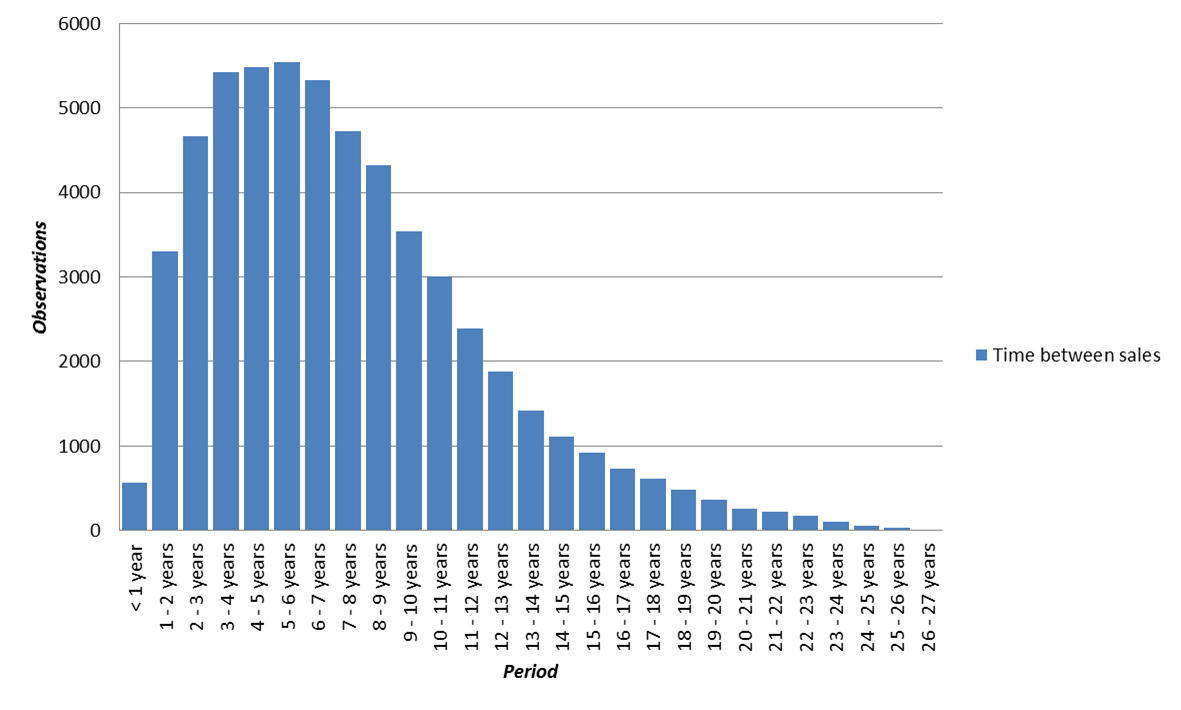
\includegraphics[width=.6\textwidth]{tbs.png}}\
                     
                  \subfloat[Time to DA]{%
                    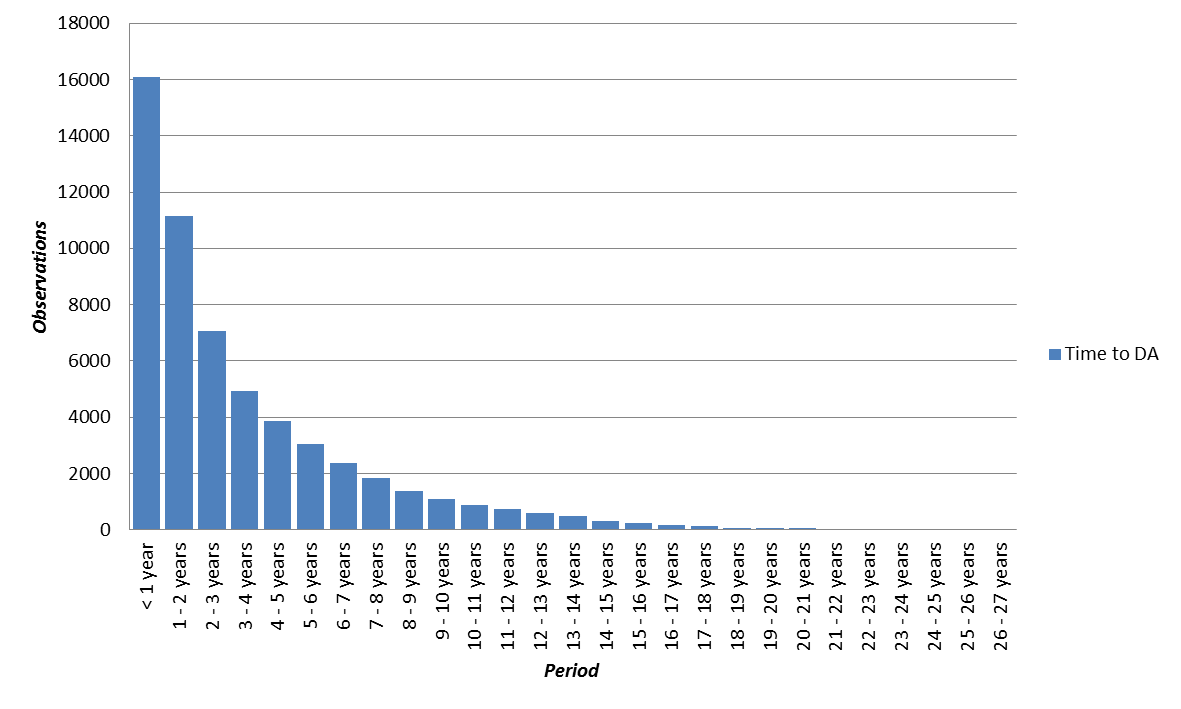
\includegraphics[width=.6\textwidth]{ttda.png}}\
                    
                \subfloat[Time to subsequent sale post DA]{%
                    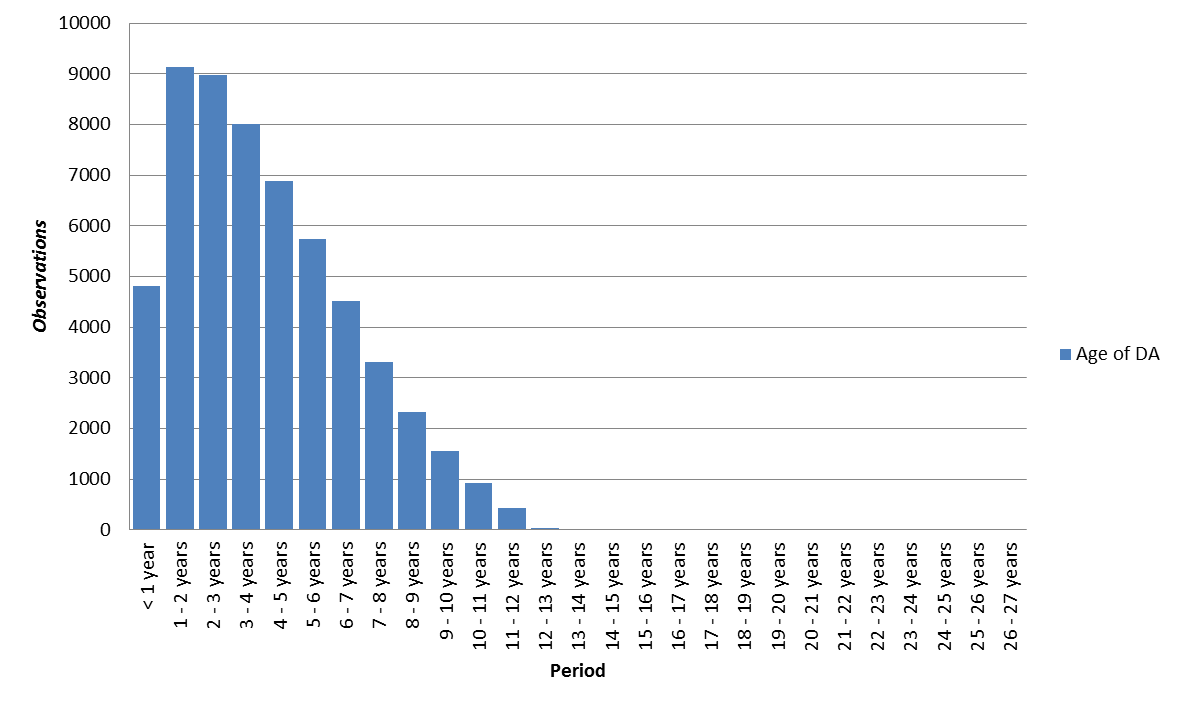
\includegraphics[width=.6\textwidth]{ageda.png}}\
                 \caption{\small{Panels (A), (B) and (C) show the distributions of time between sale, time to DA and time to subsequent sale post DA respectively}}
                 
                \label{fig:relative_time}
                
                \end{figure}
\end{comment}

Figure \ref{fig:Rplot_month_bet_sale_notional} shows the distribution of relative time of sales relative to DA. We see that the majority of people do home improvements within one year of purchasing their property. We also see there are some homeowners improve and who sell their homes within 2 years of purchasing. These households are likely to be investors and we there are some investors in the unimproved group as well. We also perform further analysis for investor and non-investor groups. Also there are some homeowner who improve the home and sell within two years of improvement. 

\begin{figure}[!ht]
    \centering
     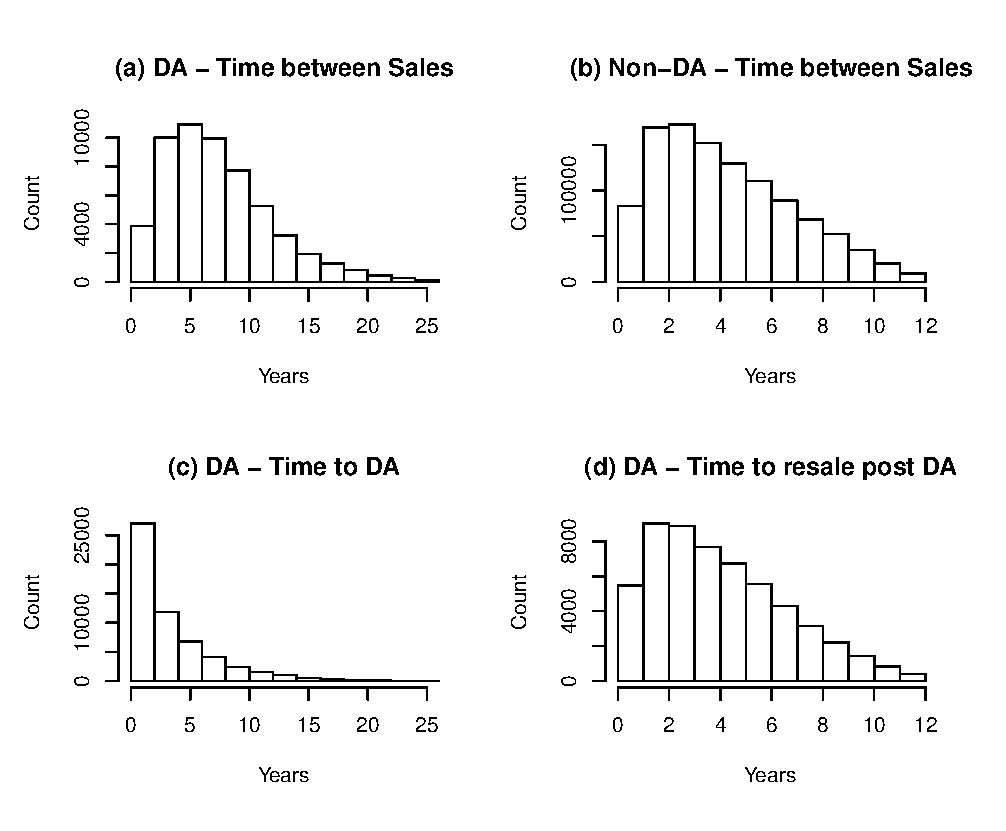
\includegraphics[width=\columnwidth]{Figures/Rplot_time_bet_sales_notional2004.eps} \par
 \caption{Time between sales for Improved vs Unimproved Homes and Time of Sale relative to DA}
 \label{fig:Rplot_month_bet_sale_notional}
\end{figure}



\begin{comment}

        \begin{figure}[!htb]
            \centering
            %\textbf{Time between Sales}\par\medskip
            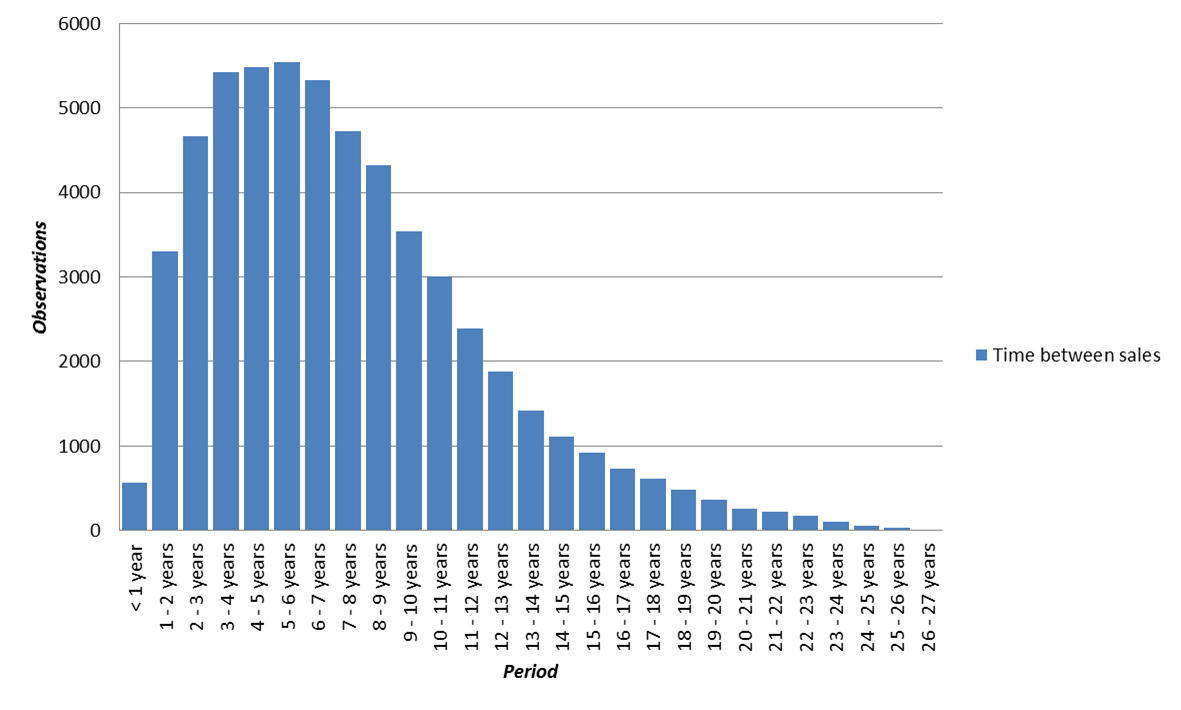
\includegraphics[scale=0.45]{tbs.png}
            \caption{Time between sales}
            \label{fig:tbs}
           % \numberwithin{figure}{section}
             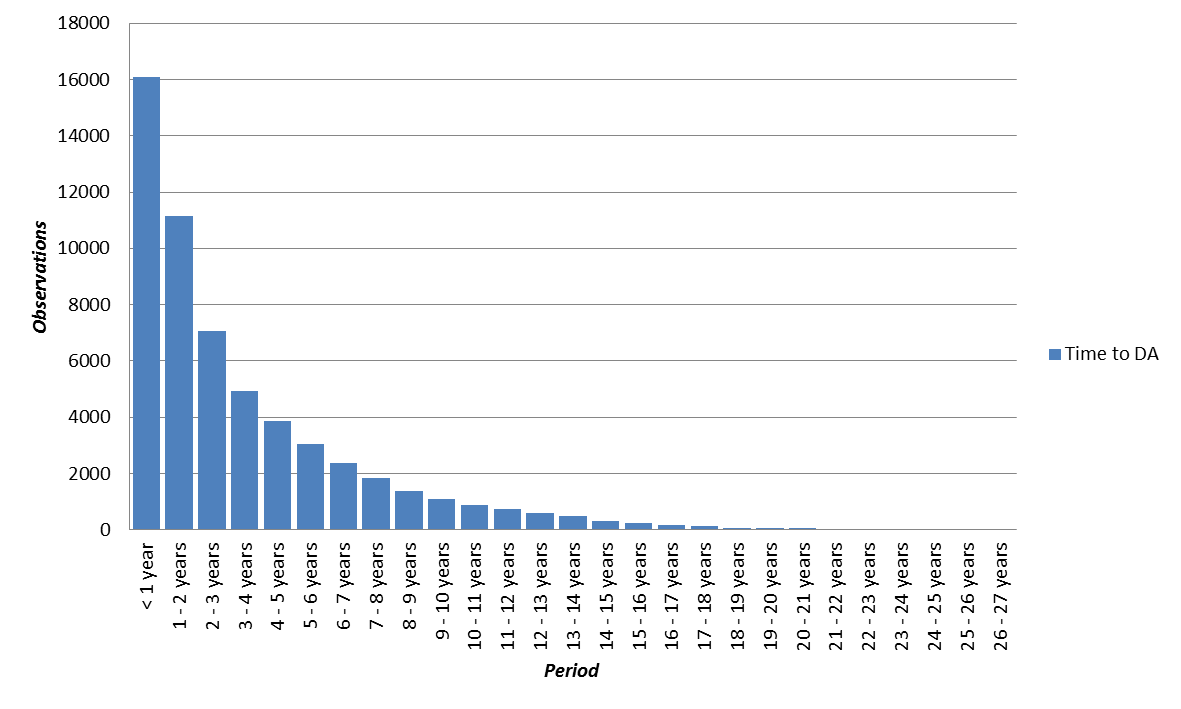
\includegraphics[scale=0.45]{ttda.png}
            \caption{Time to DA}
            \label{fig:ttda}
           % \numberwithin{figure}{section}
             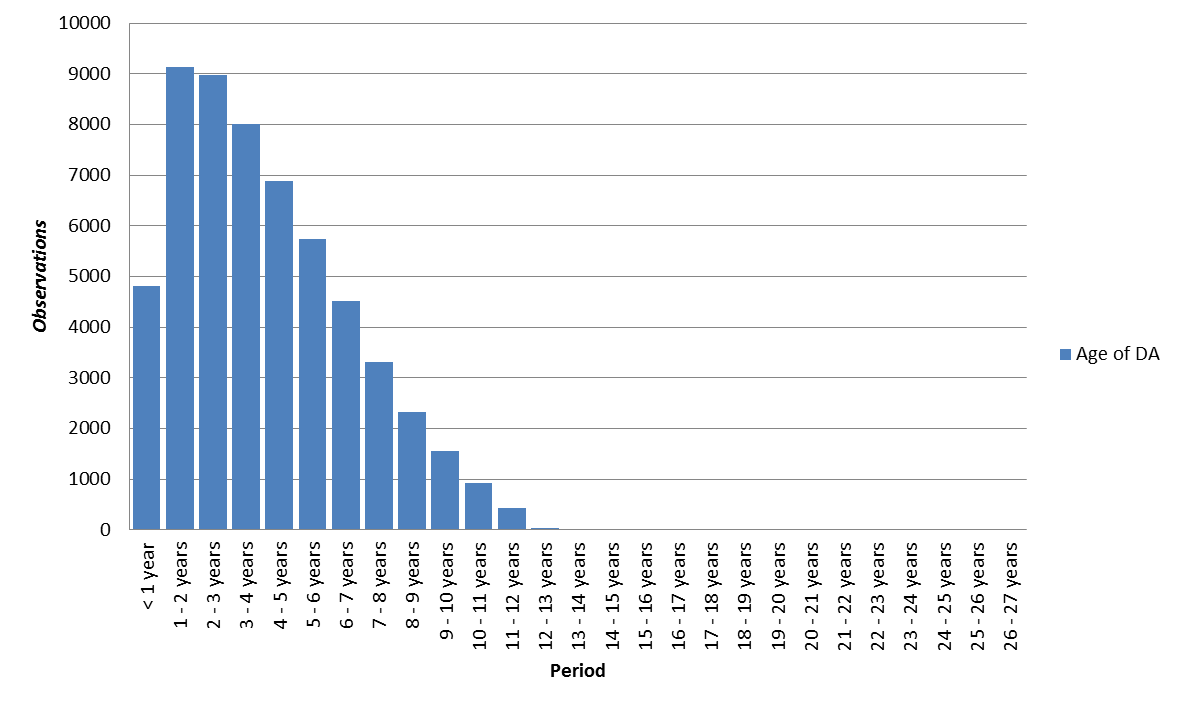
\includegraphics[scale=0.45]{ageda.png}
            \caption{Time to repeat sale after DA}
            \label{fig:ageda}
           % \numberwithin{figure}{section}
        \end{figure}
        %\floatbarrier

%\afterpage{\clearpage} %this take me to the next page
\end{comment}


Table \ref{tab:variable_statistics} shows the descriptive statistics for the main variables used in the model.

% Table generated by Excel2LaTeX from sheet '9 june 2017'
\begin{table}[!p]
  \centering
  \caption{Variable Descriptions and Sample Summary Statistics}
  \resizebox{0.93\textwidth}{!}{

  
    \begin{tabu} to \textwidth {X[2,l]X[3,l]X[0.6,c]X[0.6,c]X[0.6,c]}
    \toprule
          &       & \multicolumn{1}{c}{Overall} & \multicolumn{1}{c}{Improved} & \multicolumn{1}{c}{Unimproved} \\
\cmidrule{3-5}    Name  & Description & \multicolumn{1}{c}{Mean} & \multicolumn{1}{c}{Mean} & \multicolumn{1}{c}{Mean} \\
   &    &   \multicolumn{1}{c}{(Std. Deviation)} & \multicolumn{1}{c}{(Std. Deviation)} & \multicolumn{1}{c}{(Std. Deviation)} \\
    \midrule
     
     Number of observations &       & \multicolumn{1}{c}{1,145,547} & \multicolumn{1}{c}{55,733} & \multicolumn{1}{c}{1,089,814} \\
    &&&&\\
    
    Purchase Price & House price at first sale & \multicolumn{1}{c}{380,867} & \multicolumn{1}{c}{436,829} & \multicolumn{1}{c}{378,005} \\
          &       & \multicolumn{1}{c}{(319,547)} & \multicolumn{1}{c}{(410,073)} & \multicolumn{1}{c}{(313,949)} \\
   Expected Purchase Price at DA  &   Purchase Price indexed to DA (DA homes)    &       & \multicolumn{1}{c}{554,532} &  \\
          &       &       & \multicolumn{1}{c}{(478,355)} &  \\
    DA cost & Cost of developments as reported in development applications &       & \multicolumn{1}{c}{104,345} &  \\
          &       &       & \multicolumn{1}{c}{(165,288)} &  \\
    Purchase price (notional) & Price at purchase for unimproved homes; Indexed Purchase Price plus cost of development for DA homes & \multicolumn{1}{c}{391,670} & \multicolumn{1}{c}{658,879} & \multicolumn{1}{c}{378,005} \\
          &       & \multicolumn{1}{c}{(333,766)} & \multicolumn{1}{c}{(536,042)} & \multicolumn{1}{c}{(313,949)} \\
    Resale Price & House price at second sale & \multicolumn{1}{c}{506,030} & \multicolumn{1}{c}{887,089} & \multicolumn{1}{c}{486,542} \\
          &       & \multicolumn{1}{c}{(411,784)} & \multicolumn{1}{c}{(723,141)} & \multicolumn{1}{c}{(379,065)} \\
    SSD specific hedonic index growth rate & Annual average growth rate of statistical sub-division specific hedonic Index for property type 'house' for period 1990 - 2016 & \multicolumn{1}{c}{0.073} &       &  \\
    Log Returns & log(Resale price / Purchase price (notional)) & \multicolumn{1}{c}{0.279} & \multicolumn{1}{c}{0.304} & \multicolumn{1}{c}{0.277} \\
          &       & \multicolumn{1}{c}{(0.409)} & \multicolumn{1}{c}{(0.422)} & \multicolumn{1}{c}{(0.408)} \\
    Months between sales (notional) & No of months between sales for non modified homes; No. of months between notional purchase and resale for DA homes  &   \multicolumn{1}{c}{50.2}   & \multicolumn{1}{c}{47.7} & \multicolumn{1}{c}{50.4} \\
    
       &       & \multicolumn{1}{c}{(31.5)} & \multicolumn{1}{c}{(30.9)} & \multicolumn{1}{c}{(31.5)}\\
    
  %  DA Types & Duplex, Extension/Alteration, Garages/Sheds \& Carports,House/Single Dwelling, Multiple DA, Swimming Pool and Verandahs \& Pergolas &       &       &  \\
    \bottomrule \\[-1.8ex]
    
     \multicolumn{5}{l}{\parbox{19cm}{\LARGE This table shows the summary statistics for the main variables, directly or indirectly, used in our model. We have a total of 1.1m records used in our model with 55,733 improved homes as our treatment sample and 1.08m unimproved homes as our control sample. The average purchase price for improved and unimproved homes is \$436,829 with a standard deviation of \$410,073 and \$378,005 with a standard deviation of \$313,949. The expected purchase price at the time of DA, for improved homes is \$554,532 and with average improvement cost of \$104,345, the average notional purchase price is \$658,879 with a standard deviation of \$536,042. The notional purchase price for unimproved homes is same as the purchase price. The average resale price for improved and unimproved homes is \$887,089 with standard deviation of \$723,141 and \$486,542 with standard deviation of \$379,065 respectively. The large standard deviation of improved homes is mainly due to the different types of home improvements as some improvements for e.g. verandas/pergolas add little value while others e.g. Duplex adds more value to the homes. The average annual growth rate of Statistical Subdivision level Hedonic House Price Index used to calculate the expected purchase price and also the market return is 7.3\%. We see that the average log return of the resale price to the notional purchase price (i.e. after accounting for the cost of improvement) for improved homes is 30.4\% with a standard deviation of 42.2\%. While for unimproved homes the average log return is 27.7\% with a standard deviation of 40.8\%. In terms of univariate results, this may suggest that the return for improved homes is, on average, 2.7\% higher than unimproved homes. However, the univariate results do not control for factors such as time of purchase and resale, depreciation of the home, and property attributes such as number of beds, baths and cars which is possible in the regression model. After controlling for these factors in the regression, we find that the returns for improved homes are in fact lower, on average, than unimproved homes by 2.4\%. The average time between sales for unimproved homes is 47.7 months while for improved homes the average time between DA and resale (i.e. the time between notional purchase and resale) is 50.4 months. These are the times for which the households have consumed the housing service and allows for capturing the depreciation effect of the property.}}
    
    % the figures reported in unimproved home are for 1.08m are post 2004, but the need to be checked for constant dollars of 2016..and then update the figures above in notes..
    
    \end{tabu} %
        }
 
  \label{tab:variable_statistics}%
  
\end{table}%



%reference -- The production function for housing: evidence from france.. Combes, Duranton, Gobillon



\begin{comment}
we also need to look at the issue that we are using data starting from 1990 but the da recors are available from 2000. so we although using data from 1990 allows us to use records that have done da post 2000 period but their prev sale could be before 2000 say eg 1990. however this brings an issue taht we cannot guarantee that those records the records are in the control group of no da.. this may lead to a sample selection bias..
\end{comment}


\section{Model Estimation and Results}

The house price data is available for each individual property, however since the sale prices are observed infrequently and at different points in time, this gives rise to an unbalanced panel data. However, we take the returns of each individual property as one observation. Therefore, our data set is reduced to cross-sectional data with returns for each individual property. We estimate the model in equation \ref{eq:estimate} using the following general form,
\begin{equation}
    Y_i = DA + \beta{Mkt} + \gamma_1{Age} + \gamma_2{Age^2} + Years + Location + \mu{K} + \epsilon
\end{equation}

Where, $DA$ is the dummy variable coded as $1$ for improved homes and $0$ for unimproved homes. $Mkt$ is the market index and is captured using the hedonic house price index\footnote{The house price index provided by CoreLogic is developed at the Statistical Subdivision (SSD) level using various factors, including number of beds, baths, cars and swimming pool}. $Age$ is the time between sale and indicates how much the property has aged between sales. As the property will only start depreciating after it is built, we adjust the age by subtracting the average commencement and construction times, rounded to end of month, based on the Australian bureau of Statistics figures\footnote{\citet{abs_house_times_commence} and \citet{abs_house_times} provide average commencement time and construction times for new houses. Average construction time for swimming pool is available from \citep{hi_swimming_time}. The other values are calculated on pro-rata basis of the average costs of DA}, $Years$ is the year fixed effects at the time of improvement, $Location$ is the location fixed effects at the State level\footnote{As there could be lot of within state variation in house prices that could affect the returns, we also tested the results by controlling for the variations using SSD level fixed effects in the robustness section}. 


Since we calculate the return on each individual property, our model is reduced to a cross-sectional regression. However there are several sources of variation in the returns. One of the major sources of variations is the market appreciation. The market index variable captures the house price appreciation attributable to the market. Also since the time between the sales could be significantly different for each individual property and this could also affect house price return. Therefore the variation in the returns due to time between sales is controlled for by the Age variable. Now even though we have controlled for the market appreciation, time between sales that captures the depreciation due to aging of the property. We could still have variation in return due to the time of purchase. To account for this, we include the years fixed effects. To control for any geographical effects, we allow for location fixed effects at the State level. $K$ is a set of hedonic factors namely, number of beds, baths and cars. Since, the changes in the supply and demand of houses have been found to affect appreciation rates \citep{kiel1995effect}, these characteristics are included in the regressions as well (although the equations suggests that these cancel out).

Finally $Y_i$ is the log return of resale price over purchase price for each individual property. While, for unimproved homes the purchase price is the actual purchase price, for improved homes, the return are calculated using the notional purchase price. The notional purchase price is equal to the expected price at the time of DA\footnote{As the home improvement spending is reported as at the end of month when building approval is received and not at the time of completion, we index the actual price up to the point of DA approval month as it makes the expected value of the home expressed in the same dollar terms as the month of DA approval.}. plus the total cost of home improvement. The expected price at the time of DA approval is calculated as the actual purchase price indexed \footnote{The expected price is calculated as $E(V_0) = V_{-1} * hpi_0 / hpi_{-1}$} to the point of DA. Hence, the log returns for unimproved and improved homes is calculated as $ln[P_{+1}/P_{-1}]$ and $ln[P_{+1}/(E(P_{0})+ Cost]$ respectively, where $E(.)$ is the expectation and the expected house price at time T = 0 is given by,

$$ E(P_0) = P_{-1} * (hpi_0 / hpi_{-1}) $$ 

So at point t = 0, the notional purchase price is the actual purchase price indexed to development approval date plus the cost of DA. Note that this total price is not equivalent to the value of the home or the sale price. The sale price or value of the home will be higher as there is some additional value created from home improvement. This can be thought of as the notional purchase price. The value of the home will be equal to the notional purchase price plus the additional housing value created from the home improvement. Since homes with no improvements have no additional value, hence comparing the returns for improved homes with the unimproved homes provide us with the identification strategy for estimating returns attributable to home improvements. 

We use the notional purchase price to calculate returns for improved homes for three main reasons. Firstly it puts the purchase price and the improvement spending in the same dollar terms as at time of improvement, thereby allowing us to directly add the indexed price and cost to arrive at the notional purchase price. Secondly, since the additional value produced by the DA which is $H'$ is only identified after the completion of DA.  Any returns from the point of purchase to the point of development approval can only be attributed to the market appreciation and therefore any variation in the returns prior to development approval does not contribute to the identification of home improvement value. Finally, in improvement types like building a new house or building a new duplex, the homeowners demolish the existing building and develop a new house from scratch. However the existing building, after accounting for the depreciation should have some residual building value, $B_0$ (the non-durable consumption) plus the housing service value, $H_0$ (the durable consumption). With the demolition of the old building, while the land value, $\alpha$ remains intact, the non-durable and durable consumption value at time of DA $(B_0 + H_0)$ is reduced to zero. This is the opportunity cost if the land were to be used for purposes other than residential. However, as the homeowner redevelops a house, the value of housing $H$ is regained and there is some additional housing value $H'$ created\footnote{Assuming that the homeowner builds a better home than the previous one.}. Therefore the opportunity cost of DA is only $B_0$. And cost is inseparable and observed implicitly in the Expected value of the home, calculated using the market index, at point of DA. Therefore to fully account for the costs, we need to calculate the expected purchase price at the time of DA\footnote{In case of other improvement types, the existing value of land, building and housing service remains intact, therefore there is no direct opportunity cost. When the home owner carries out development, the only cost is C, the cost of home improvement and the unobserved value created from home improvement is $H'$ which is indirectly observed in the resale price. Therefore there is no direct impact for to the other types of home improvements.}. 

Now, since the development actually happens any time between a purchase and a resale, So at the time of DA, there is a cost incurred, which is observed at the time of building approval received and there is a value produced by completing the development. This value is equal to the building value (i.e. the amount spent for the construction of the building) plus the value of additional housing service). The cost of construction is observed but the value of housing service is unobserved at the time of DA. When the property sells subsequent DA, the additional value produced by DA will be implicitly observed in the resale price. This provides our identification strategy. The identification comes from controlling for the common sources of variation in the house price that affect the returns. A major variation in the house price returns will be attributed to the market appreciation which is captured using the return on the house price index. Another source of variation is after how long does one sell their home post home improvement. This variable captures the depreciation effect of aging of the existing and the additional building value created through improvement. Another potential source of variation in the returns could be the land area. Due to the sparsely available information on land area, we use number of beds, baths and cars to proxy for the land area. As our model calculates returns on notional purchase price, any variations in returns between purchase and point of DA are already captured in the expected price using the SSD index and therefore the time to DA does not contribute to model identification. 

Once the common sources of variations between improved and unimproved homes are controlled for, the difference in the returns would then only be attributable to the home improvement. Hence in order to identify that variation, we simply use a binary dummy variable to capture the differences in the returns between improved and unimproved homes.

Table \ref{tab:results} shows the estimation results for different model specifications\footnote{Robust standard errors are reported in parenthesis and the significance of the variables is adjusted according to the robust standard errors}. 

\clearpage
\newgeometry{margin=1in}
% Table created by stargazer v.5.2 by Marek Hlavac, Harvard University. E-mail: hlavac at fas.harvard.edu
% Date and time: Fri, Jun 30, 2017 - 10:00:05 AM
% Requires LaTeX packages: dcolumn rotating 


\begin{sidewaystable}[!htbp] \centering 
  \caption{Main Model Results} 
  \label{tab:results} 
  \resizebox{\textwidth}{!}{
  \begin{threeparttable}

\begin{tabular}{@{\extracolsep{5pt}}lD{.}{.}{-3} D{.}{.}{-3} D{.}{.}{-3} D{.}{.}{-3} D{.}{.}{-3} D{.}{.}{-3} } 
\\[-1.8ex] 
\toprule \\[-1.8ex] 
\\[-1.8ex] & \multicolumn{6}{c}{Log(Resale Price/Purchase Price (Notional))} \\ 
\\[-1.8ex] & \multicolumn{1}{c}{(1)} & \multicolumn{1}{c}{(2)} & \multicolumn{1}{c}{(3)} & \multicolumn{1}{c}{(4)} & \multicolumn{1}{c}{(5)} & \multicolumn{1}{c}{(6)}\\ 
\midrule \\[-1.8ex] 
 DA &  &  &  &  & -0.019^{***} & -0.024^{***} \\ 
  &  &  &  &  & (0.002) & (0.002) \\ 
  %& & & & & & \\ 
 Carports/Garages/Sheds & -0.022^{***} & -0.021^{***} & -0.021^{***} & -0.025^{***} &  &  \\ 
  & (0.007) & (0.007) & (0.007) & (0.007) &  &  \\ 
  %& & & & & & \\ 
 Duplex & 0.094^{***} & 0.097^{***} & 0.098^{***} & 0.101^{***} &  &  \\ 
  & (0.013) & (0.013) & (0.013) & (0.013) &  &  \\ 
  %& & & & & & \\ 
 Extension/Alteration & 0.001 & 0.001 & 0.000 & -0.001 &  &  \\ 
  & (0.004) & (0.004) & (0.004) & (0.004) &  &  \\ 
  %& & & & & & \\ 
 House/Single Dwelling & -0.105^{***} & -0.101^{***} & -0.100^{***} & -0.102^{***} &  &  \\ 
  & (0.007) & (0.007) & (0.007) & (0.007) &  &  \\ 
  %& & & & & & \\ 
 Multiple DA & -0.018^{***} & -0.012^{*} & -0.011^{*} & -0.017^{***} &  &  \\ 
  & (0.006) & (0.006) & (0.006) & (0.006) &  &  \\ 
  %& & & & & & \\ 
 Swimming Pool & -0.001 & 0.004 & 0.004 & -0.005 &  &  \\ 
  & (0.003) & (0.003) & (0.003) & (0.003) &  &  \\ 
  %& & & & & & \\ 
 Verandahs/Pergolas & -0.039^{***} & -0.037^{***} & -0.038^{***} & -0.042^{***} &  &  \\ 
  & (0.004) & (0.004) & (0.004) & (0.004) &  &  \\ 
  %& & & & & & \\ 
 MktReturn & 0.804^{***} & 0.923^{***} & 0.922^{***} & 0.924^{***} & 0.923^{***} & 0.925^{***} \\ 
  & (0.003) & (0.003) & (0.003) & (0.003) & (0.003) & (0.003) \\ 
  %& & & & & & \\ 
 Months between sales &  & -0.001^{***} & -0.002^{***} & -0.002^{***} & -0.002^{***} & -0.002^{***} \\ 
  &  & (0.000) & (0.000) & (0.000) & (0.000) & (0.000) \\ 
  %& & & & & & \\ 
 Months between sales squared &  &  & 0.000^{***} & 0.000^{***} & 0.000^{***} & 0.000^{***} \\ 
  &  &  & (0.000) & (0.000) & (0.000) & (0.000) \\ 
  %& & & & & & \\ 
 No. of beds (resale) & 0.026^{***} & 0.027^{***} & 0.026^{***} &  & 0.026^{***} &  \\ 
  & (0.001) & (0.001) & (0.001) &  & (0.001) &  \\ 
  %& & & & & & \\ 
 No. of baths (resale) & 0.058^{***} & 0.059^{***} & 0.059^{***} &  & 0.059^{***} &  \\ 
  & (0.001) & (0.001) & (0.001) &  & (0.001) &  \\ 
  %& & & & & & \\ 
 No. of cars (resale) & 0.004^{***} & 0.006^{***} & 0.006^{***} &  & 0.006^{***} &  \\ 
  & (0.000) & (0.000) & (0.000) &  & (0.000) &  \\ 
  %& & & & & & \\ 
 No. of beds (purchase) & -0.032^{***} & -0.033^{***} & -0.033^{***} &  & -0.032^{***} &  \\ 
  & (0.001) & (0.001) & (0.001) &  & (0.001) &  \\ 
  %& & & & & & \\ 
 No. of baths (purchase) & -0.069^{***} & -0.069^{***} & -0.069^{***} &  & -0.068^{***} &  \\ 
  & (0.001) & (0.001) & (0.001) &  & (0.001) &  \\ 
  %& & & & & & \\ 
 No. of cars (purchase) & -0.015^{***} & -0.016^{***} & -0.016^{***} &  & -0.016^{***} &  \\ 
  & (0.000) & (0.000) & (0.000) &  & (0.000) &  \\ 
  %& & & & & & \\ 
 Change in \# of beds &  &  &  & 0.029^{***} &  & 0.029^{***} \\ 
  &  &  &  & (0.001) &  & (0.001) \\ 
  %& & & & & & \\ 
 Change in \# of baths &  &  &  & 0.063^{***} &  & 0.062^{***} \\ 
  &  &  &  & (0.001) &  & (0.001) \\ 
  %& & & & & & \\ 
 Change in \# of cars &  &  &  & 0.010^{***} &  & 0.010^{***} \\ 
  &  &  &  & (0.000) &  & (0.000) \\ 
  %& & & & & & \\ 
 Constant & 0.088^{***} & 0.114^{***} & 0.129^{***} & 0.078^{***} & 0.129^{***} & 0.078^{***} \\ 
  & (0.002) & (0.002) & (0.003) & (0.002) & (0.003) & (0.002) \\ 
  %& & & & & & \\ 
Year Fixed Effects & Yes & Yes & Yes & Yes & Yes &  \\ 
Location Fixed Effects & Yes & Yes & Yes & Yes & Yes &  \\ 
Observations & \multicolumn{1}{c}{517,011} & \multicolumn{1}{c}{517,011} & \multicolumn{1}{c}{517,011} & \multicolumn{1}{c}{517,011} & \multicolumn{1}{c}{517,011} & \multicolumn{1}{c}{517,011} \\ 
Adjusted R$^{2}$ & \multicolumn{1}{c}{0.281} & \multicolumn{1}{c}{0.289} & \multicolumn{1}{c}{0.290} & \multicolumn{1}{c}{0.287} & \multicolumn{1}{c}{0.289} & \multicolumn{1}{c}{0.287} \\ 
F Statistic & \multicolumn{1}{c}{6,528.365$^{***}$ (df = 31; 516979)} & \multicolumn{1}{c}{6,580.655$^{***}$ (df = 32; 516978)} & \multicolumn{1}{c}{6,398.490$^{***}$ (df = 33; 516977)} & \multicolumn{1}{c}{6,954.690$^{***}$ (df = 30; 516980)} & \multicolumn{1}{c}{7,793.277$^{***}$ (df = 27; 516983)} & \multicolumn{1}{c}{8,663.804$^{***}$ (df = 24; 516986)} \\ 


%F Statistic & \multicolumn{1}{H}{6,097.764$^{***}$ (df = 27; 1145334)} & \multicolumn{1}{H}{6,085.191$^{***}$ (df = 30; 1035385)} & \multicolumn{1}{H}{6,111.101$^{***}$ (df = 33; 525110)} & \multicolumn{1}{H}{6,167.475$^{***}$ (df = 34; 525109)} & \multicolumn{1}{c}{6,007.371$^{***}$ (df = 35; 525108)} & \multicolumn{1}{c}{6,493.052$^{***}$ (df = 32; 525111)} & \multicolumn{1}{c}{7,225.539$^{***}$ (df = 29; 525114)} & \multicolumn{1}{c}{7,964.678$^{***}$ (df = 26; 525117)} \\ 

\bottomrule \\[-1.8ex] 
%\multicolumn{9}{p{1.2\textwidth}}{Robust standard errors are reported in parentheses, Significance of variables is adjusted accordingly. *** 0.1\% significance ** 1\% significance * 5\% significance. We have a total of 1,145,547 (55,733 for treatment and 1,089,814 for control sample) possible observation with deviation accounted for by missing data.} \\ 
\end{tabular}

 \begin{tablenotes}[para,flushleft]
  \LARGE
      Notes: Robust standard errors are reported in parentheses, Significance of variables is adjusted accordingly. *** 0.1\% significance ** 1\% significance * 5\% significance. We have a total of 1,119,419 (55,733 for treatment and 1,063,686 for control sample) possible observation with deviation accounted for by missing data.
\end{tablenotes}    

    \end{threeparttable}


}
\end{sidewaystable} 
\restoregeometry

All model specifications allow for year and location fixed effect. Since the returns are modelled in log form, the actual interpretation of coefficients is ($e^{\hat{\beta}}-1$). The estimated coefficients are close to actual for small values of $\hat{\beta}$.  Model 1 is the basic model with house price log returns regressed only on the market index and no controls. The coefficient on the MktReturn is 0.749 which indicates that 75\% of the appreciation in the house prices is due to the market. Model 2 includes the property attributes at the time of resale and model 3 includes the property attributes for both, at the time of resale and purchase. The coefficients on both, purchase and resale attributes are significant, with values for number of beds, baths and cars at resale as 2.6\%, 5.8\% and 0.4\% and -3.2\%, -6.2\% and -1.5\% at time of purchase respectively. This indicates that, other factors constant, the return is higher if one buys a smaller house and sells a bigger house and vice-versa. In model 3, we see that the variation captured by the market returns has improved to 80\%. 

In model 4, we include age as a linear term while in model 5 we include age as a quadratic term. The age captures the depreciation effect of the property attributed to the non-durable consumption. The coefficient on age in the linear form indicates that the returns on the property decreases by 0.1\% every month due to the depreciation. In the quadratic form, the coefficient on age is -0.2\% while the coefficient on squared age is positive. Since the age is measured in months, the coefficient on the quadratic term (the curvature) is quite small but statistically significant and therefore we include the squared term in the full model. The coefficients in the attributes at the time of purchase and resale are consistent with the previous models. Also the variation in the returns captured by the market appreciation further improves to 92\%. 

Models 1 to 5, present returns for each of the home improvement types, relative to unimproved homes. Models 5 is a full model with control for market appreciation and other attributes. Depending on the model specification, the returns on each of improvement types are not attributed to the market appreciation and other attributes as they are already controlled for explicitly. Also any omitted or unobserved (deterministic) factors will be captured in the constant. Hence the returns on each of the improvement types are over and above the returns for unimproved homes. 

The results show that the returns for carports are negative and mostly insignificant across models specifications. The coefficient on duplexes, in the full model, suggests that the return for a duplex is 9.8\% higher than the unimproved homes. Also, across all models, the results for duplexes are consistently positive and significant ranging between 8.4\% to 18\%. For Extension/Alterations, the returns are insignificant across models with controls. In case of House/Single Dwelling, the returns are consistently negative and strongly significant in all model specifications. The full model coefficient on House/Single Dwelling is -0.10 indicating that the returns for House/Single Dwelling is around 10\% lower than unimproved homes. For Multiple DAs, on average, the results are mostly negative and significant across models. In the full model, the return on Multiple DAs is 1.1\% lower than the unimproved homes. In case of Swimming pools, when there is no control for attributes at the time of purchase, the returns are almost 18\% and 14\% higher than unimproved homes. However when we control for the purchase attributes, the returns become insignificant. And when we include depreciation, the returns are marginally positive and significant at 0.4\%. For verandas/pergolas, the returns are mostly negative and strongly significant. In the full model, the return on verandas and pergolas is 3.8\% lower than unimproved homes.

The model 1 does not have any control attributes and therefore it assumes that all properties are bought and sold are of the same size. Model 2 controls for the attributes at the time of resale and therefore assumes that all homes bought are of the same size. And in model 3, we control for the size at both, the time of purchase and resale. However, although we account for the size of the house using number of beds, baths and cars, the size in terms of land area could still vary significantly and therefore have some unidentified variations in returns. 

The attributes at the time of resale are likely to be higher than the time of purchase, if the homeowner carries out development, or remain the same if they do nothing. In models 3, 4 and 5, we have both, attributes at the time of resale and purchase and therefore they are quite likely to be correlated. Hence, we also examine the model with alternate specification, in model 6, where we take change in the corresponding attributes. This way we avoid the problem of multi-collinearity. However, due to change in attributes, we loose valuable information on the absolute level of attributes which serves as a proxy for the land area. Implicitly, this model assumes that returns for a homeowner who buys a 1 bedroom and sell a two bedroom will be the same as for someone who buys a two bedroom and sells a three bedroom house as the change in no. of bedrooms is the same in both cases. Hence, we present the results on both model specifications as they have their own merits.

The finding in the alternate model specification are also consistent with overall results. The returns on carports/garages/sheds and verandas/pergolas is 2.5\% and 4.2\% lower than the unimproved homes respectively. For Duplex the returns are 10.1\% higher than unimproved homes. For extension/alteration and swimming pools, the returns are not significantly different from unimproved homes. In case of House/Single Dwelling, the return are strongly negative by 10.2\% as compared to unimproved homes. Finally, for multiple DAs, the average returns are 4.2\% below unimproved homes. The coefficient on the mktreturn is 92.2\% same as the model 5. The change in no. of beds, baths and cars are all positive indicating that greater the difference between size of the house before and after improvement, higher are the returns. 

Overall, across different home improvement types, we find that the returns for carports/garages/sheds, multiple DAs and verandas/pergolas are negative relative to the unimproved homes while for house/single dwelling, the return is strongly negative. The returns for extension/alterations and swimming pools is not significantly different from unimproved homes. In contrast, the return for duplexes is strongly positive.

One of the reasons that explains why the returns on house/single dwelling, is strongly negative is the high opportunity cost. In building a new house, unlike extension/alteration where the homeowner produces additional housing by building on top of the existing value of the building, the homeowner needs to demolish the exiting building and then build the house from the scratch and therefore in the process looses the entire residual value building $B_0$ (the non-durable consumption value) plus the value of housing service $H_0$ (durable consumption). 

According to \citet{potepan1989interest}, there are technological constraints, for example, the presence of existing housing constraints the home improvement by impeding the application of certain construction techniques common in new housing production. For relatively modest increases in housing demand, this technological difference is probably negligible. For sizable increases, this technological constraint results in higher average costs in home improvement. Therefore in building the new house there is some inherent value due to the efficiency gains as compared to extension/alterations. Hence, the losses in building the new house are reduced to the extent of the efficiency gains availed from lack of impediment.

Like building a new house, duplex also has high opportunity cost as it also requires to demolish the old property and therefore loose all residual value of the existing building. But the returns on duplexes much higher than the unimproved homes? The is because of the land split. All the properties that are converted into a duplex as part of improvement, are purchased as a single block of land that was originally for single family dwelling. When applying for development application for duplexes, homeowners could split the block of land and convert it to a dual occupancy use\footnote{For example, if the original property is on 1/13 Cragg street, then after the split the two duplexes will be addressed - 1/13 and 1A/13 Cragg Street.}. Now homeowners are able to build two identical duplexes for two single families. The homeowners can sell one duplex and reside in the other or sell both\footnote{if the homeowner sells only one duplex then we only have observed record and if they sell both, then we just take one record and double the resale price.}.  Either way, the homeowners have created twice as much equity from selling two duplexes. However the resale price observed in the data set corresponds only to one duplex\footnote{This is because if the other duplex is not sold or valued or financed, then that duplex is not recorded in CoreLogic database}. Therefore for duplexes, we double the resale price to adjust for the double equity. Hence, the return on Duplexes are strongly positive although partly offset by the losses due to lost residual value.

When homeowners carry out alteration/extension, the fundamental cost of the improvement they should pay for is the cost of building materials plus the labour cost. With the completion of development, there is an additional value of housing service produced for the homeowners which is unobserved at that time but observed implicitly at the time of resale. Some portion of this expected value created from home improvement is priced into the cost of development. This could also be the contribution factor for why the returns for alteration/extension is insignificant.
Apart from this there is some portion of the building value that is depreciated away and therefore we find, insignificant profits after controlling for market appreciation. In case of swimming pool, in addition to the reasons discussed for extension/alterations, the insignificant returns can be attributed to the perceived cost of operating the swimming pool on a regular basis and therefore, depending on the preferences, prospective buyers may not value the utility of the swimming pool and therefore the homeowner may not get a better resale price.

Models 7 and 8 are the aggregate level results corresponding to model specifications 5 and 6 respectively. The coefficient on DA dummy represents the returns for improved homes relative to unimproved homes. On average, we find that, based on model 7 and 8, the returns for improved homes are on average 1.9\% and 2.4\% lower than the unimproved homes respectively. Therefore homeowners who do nothing are relatively better off than those who improve their homes. 

\clearpage
\section{Further Analysis}

In the previous section, we compared the returns for all improved homes with unimproved homes and found that the returns for improved homes is lower than unimproved homes. In this section, we perform further analysis to examine how the returns for homeowners with an investment motive perform for improved homes with respect to the unimproved homes. People who buy and sell the property within 2 years are likely to have an investment motive at the onset\footnote{We take two years as a good approximation for home buyers intention to buy the property with an investment motive. Any longer period increases the chances that the homeowner did not buy the property with a view of investment but rather bought the property for self consumption.} and therefore we identify homeowners that buy and sell the property within 2 years as investors and those who buy and sell in more than 2 years as non-investors. 

% Table created by stargazer v.5.2 by Marek Hlavac, Harvard University. E-mail: hlavac at fas.harvard.edu
% Date and time: Wed, Jun 21, 2017 - 11:23:41 AM
% Requires LaTeX packages: dcolumn rotating 
\begin{table}[!p] \centering 
  \caption{Results for Speculator Type I and Non-Speculator Groups} 
  \label{tab:results_s0_investor_da_interaction} 
  \resizebox{0.7\textwidth}{!}{
\begin{tabular}{@{\extracolsep{5pt}}lD{.}{.}{-3} D{.}{.}{-3} } 
\\[-1.8ex] 
\toprule \\[-1.8ex] 
\\[-1.8ex] & \multicolumn{2}{c}{Log(Resale Price/Purchase Price (Notional))} \\ 
\\[-1.8ex] & \multicolumn{1}{c}{(1)} & \multicolumn{1}{c}{(2)}\\ 
\midrule \\[-1.8ex] 
 DA & -0.021^{***} & -0.025^{***} \\ 
  & (0.002) & (0.002) \\ 
  & & \\ 
 Investor & 0.007^{***} & 0.007^{***} \\ 
  & (0.001) & (0.001) \\ 
  & & \\ 
  DA:Investor & 0.025^{***} & 0.026^{***} \\ 
  & (0.006) & (0.006) \\ 
  & & \\ 
 MktReturn & 0.921^{***} & 0.923^{***} \\ 
  & (0.003) & (0.003) \\ 
  & & \\ 
 Age & -0.002^{***} & -0.002^{***} \\ 
  & (0.000) & (0.000) \\ 
  & & \\ 
 Age Square & 0.000^{***} & 0.000^{***} \\ 
  & (0.000) & (0.000) \\ 
  & & \\ 
 No. of beds (Resale) & 0.026^{***} &  \\ 
  & (0.001) &  \\ 
  & & \\ 
 No. of baths (Resale) & 0.058^{***} &  \\ 
  & (0.001) &  \\ 
  & & \\ 
 No. of cars (Resale) & 0.006^{***} &  \\ 
  & (0.000) &  \\ 
  & & \\ 
 No. of beds (Purchase) & -0.033^{***} &  \\ 
  & (0.001) &  \\ 
  & & \\ 
 No. of baths (Purchase) & -0.067^{***} &  \\ 
  & (0.001) &  \\ 
  & & \\ 
 No. of cars (Purchase) & -0.016^{***} &  \\ 
  & (0.000) &  \\ 
  & & \\ 
 Change in \# of beds &  & 0.029^{***} \\ 
  &  & (0.001) \\ 
  & & \\ 
 Change in \# of baths &  & 0.062^{***} \\ 
  &  & (0.001) \\ 
  & & \\ 
 Change in \# of cars &  & 0.010^{***} \\ 
  &  & (0.000) \\ 
  & & \\ 
 Constant & 0.126^{***} & 0.075^{***} \\ 
  & (0.005) & (0.004) \\ 
  & & \\ 
Year Fixed Effects & Yes & Yes \\ 
Location Fixed Effects & Yes & Yes \\ 
Observations & \multicolumn{1}{c}{525,144} & \multicolumn{1}{c}{525,144} \\ 
Adjusted R$^{2}$ & \multicolumn{1}{c}{0.285} & \multicolumn{1}{c}{0.283} \\ 
F Statistic & \multicolumn{1}{c}{6,761.652$^{***}$} & \multicolumn{1}{c}{7,398.417$^{***}$ } \\ 
 & \multicolumn{1}{c}{(df = 31; 525112)} & \multicolumn{1}{c}{(df = 28; 525115)} \\ 
\bottomrule \\[-1.8ex] 
\multicolumn{3}{l}{Notes: *** 0.1\% significance ** 1\% significance * 5\% significance}\\
\multicolumn{3}{l}{Robust standard errors in parentheses.} \\
\end{tabular}
}
\end{table}

For the homeowner with improved homes, we classify investors into two types. Investor type I are those who have an investment motive right at the onset and therefore buy the property, improve and then sell within 2 years of buying\footnote{homeowner who buy with an investment motive of renting the property and sell in more than 2 years from buying are treated as non-investors since the income they generate is equivalent to someone else consuming the property on owner's behalf.}. Investor type II are those homeowners who buy the property not with a view to sell the property in the near term but to live and consume the housing service and at some point later improve the property and then sell it within 2 years of improvement. These investors are those who improve and then sell in less than 2 years\footnote{The time of 2 years is calculated from the date of DA approval and not the completion of home improvement as this time closely represents the time of their decision to improve and most probably their intent to sell post improvement.} from the time of improvement. 

\subsection{Investor Type I}

Table \ref{tab:results_s0_investor_da_interaction} shows the results of the model for investor type I and non investor groups. DA is the dummy variable equal to 1 for improved homes and 0 for unimproved homes. Investor equals 1 if time between actual purchase and resale is less than 2 years and 0 otherwise. DA*Investor is the interaction term. Models 1 and 2 are the full model specifications at aggregate level with interaction terms. The coefficient on other model variables are all consistent with the main model results.

In models 1 and 2, for homeowners who are non-investors, we find that results confirm our main findings. The returns for improved homes is 2.1\% and 2.5\% lower than unimproved homes respectively. However, for the investor group, we find that the returns for improved homes are significant and higher than unimproved homes by 0.4\% (-0.021 + 0.025) and 0.1\% (-0.025 + 0.026) respectively.

If we compare across investor and non-investor group, for unimproved homes, the return for investor group is 0.7\% higher than the non-investor group in both model specifications 1 and 2. If we look at improved homes, then the returns for investor is 3.2\% (0.007 + 0.025) and 3.3\% (0.007 +0.026) higher than non-investors respectively.

The homeowner who do not improve their home and buy and sell within 2 years have higher returns than those who buy and sell in more than 2 years. Therefore the gap between returns of investor and non investor group is much higher for improved homes than unimproved homes. This suggests that, in contrast to the main results, homeowners who have investment motive and improve their homes are better off than homeowners with investment motive but do not improve their home.

In table \ref{tab:results_s0_investor_da_type}, we split the results by improvement types focus on investors only. We present the findings in models 1 to 6 that correspond to the model specifications in the main results. The results show that returns for carports/garages/sheds has improved from significantly negative in the main results to being not significantly different from unimproved homes. The returns for Duplex is mostly around 8\% higher which is similar to the main results where the duplex return is around 10\% higher than unimproved homes. 

% Table created by stargazer v.5.2 by Marek Hlavac, Harvard University. E-mail: hlavac at fas.harvard.edu
% Date and time: Wed, Jun 21, 2017 - 10:58:59 AM
% Requires LaTeX packages: dcolumn rotating 
\begin{table}[!p] \centering 
  \caption{Results for Speculator I by DA works} 
  \label{tab:results_s0_investor_da_type} 
  \resizebox{\textwidth}{!}{
\begin{tabular}{@{\extracolsep{5pt}}lHH D{.}{.}{-3} D{.}{.}{-3} D{.}{.}{-3} D{.}{.}{-3} } 
\\[-1.8ex] 
\toprule \\[-1.8ex] 
\\[-1.8ex] & \multicolumn{6}{c}{Log(Resale Price/Purchase Price (Notional))} \\ 
\\[-1.8ex] & \multicolumn{1}{H}{(1)} & \multicolumn{1}{H}{(2)} & \multicolumn{1}{c}{(1)} & \multicolumn{1}{c}{(2)} & \multicolumn{1}{c}{(3)} & \multicolumn{1}{c}{(4)}\\ 
\midrule \\[-1.8ex] 

 Carports/Garages/Sheds & -0.063^{***} & -0.049^{**} & 0.018 & 0.012 & 0.013 & 0.009 \\ 
  & (0.023) & (0.024) & (0.024) & (0.024) & (0.024) & (0.024) \\ 
  %& & & & & & \\ 
 Duplex & 0.139^{***} & 0.087^{***} & 0.066^{***} & 0.087^{***} & 0.080^{***} & 0.082^{***} \\ 
  & (0.014) & (0.014) & (0.017) & (0.017) & (0.017) & (0.017) \\ 
  %& & & & & & \\ 
 Extension/Alteration & 0.082^{***} & 0.048^{***} & 0.058^{***} & 0.053^{***} & 0.055^{***} & 0.054^{***} \\ 
  & (0.008) & (0.009) & (0.010) & (0.010) & (0.010) & (0.010) \\ 
  %& & & & & & \\ 
 House/Single Dwelling & -0.111^{***} & -0.158^{***} & -0.121^{***} & -0.108^{***} & -0.110^{***} & -0.113^{***} \\ 
  & (0.012) & (0.011) & (0.017) & (0.017) & (0.017) & (0.017) \\ 
  %& & & & & & \\ 
 Multiple\_DA & 0.021 & -0.028^{*} & 0.016 & 0.024 & 0.024 & 0.019 \\ 
  & (0.015) & (0.015) & (0.020) & (0.021) & (0.021) & (0.020) \\ 
  %& & & & & & \\ 
 Swimming Pool & 0.041^{***} & 0.020 & 0.011 & 0.012 & 0.013 & 0.005 \\ 
  & (0.014) & (0.014) & (0.009) & (0.009) & (0.009) & (0.009) \\ 
  %& & & & & & \\ 
 Verandahs/Pergolas & -0.049^{***} & -0.042^{***} & 0.005 & -0.003 & -0.003 & -0.006 \\ 
  & (0.012) & (0.013) & (0.012) & (0.012) & (0.012) & (0.012) \\ 
  %& & & & & & \\ 
 MktReturn & 0.796^{***} & 0.829^{***} & 0.868^{***} & 0.931^{***} & 0.933^{***} & 0.938^{***} \\ 
  & (0.009) & (0.009) & (0.009) & (0.010) & (0.010) & (0.010) \\ 
  %& & & & & & \\ 
 Age &  &  &  & -0.003^{***} & -0.006^{***} & -0.006^{***} \\ 
  &  &  &  & (0.000) & (0.001) & (0.001) \\ 
  %& & & & & & \\ 
 Age Square &  &  &  &  & 0.000^{***} & 0.000^{***} \\ 
  &  &  &  &  & (0.000) & (0.000) \\ 
  %& & & & & & \\ 
 No. of beds (Resale) &  & 0.020^{***} & 0.031^{***} & 0.031^{***} & 0.031^{***} &  \\ 
  &  & (0.001) & (0.002) & (0.002) & (0.002) &  \\ 
  %& & & & & & \\ 
 No. of baths (Resale) &  & 0.050^{***} & 0.058^{***} & 0.059^{***} & 0.059^{***} &  \\ 
  &  & (0.002) & (0.002) & (0.002) & (0.002) &  \\ 
  %& & & & & & \\ 
 No. of cars (Resale) &  & -0.010^{***} & 0.004^{***} & 0.004^{***} & 0.004^{***} &  \\ 
  &  & (0.001) & (0.001) & (0.001) & (0.001) &  \\ 
  %& & & & & & \\ 
 No. of beds (Purchase) &  &  & -0.035^{***} & -0.035^{***} & -0.035^{***} &  \\ 
  &  &  & (0.002) & (0.002) & (0.002) &  \\ 
  %& & & & & & \\ 
 No. of baths (Purchase) &  &  & -0.067^{***} & -0.068^{***} & -0.068^{***} &  \\ 
  &  &  & (0.002) & (0.002) & (0.002) &  \\ 
  %& & & & & & \\ 
 No. of cars (Purchase) &  &  & -0.015^{***} & -0.015^{***} & -0.015^{***} &  \\ 
  &  &  & (0.001) & (0.001) & (0.001) &  \\ 
  %& & & & & & \\ 
 Change in \# of beds &  &  &  &  &  & 0.033^{***} \\ 
  &  &  &  &  &  & (0.002) \\ 
  %& & & & & & \\ 
 Change in \# of baths &  &  &  &  &  & 0.062^{***} \\ 
  &  &  &  &  &  & (0.002) \\ 
  %& & & & & & \\ 
 Change in \# of cars &  &  &  &  &  & 0.009^{***} \\ 
  &  &  &  &  &  & (0.001) \\ 
  %& & & & & & \\ 
 Constant & 0.059^{***} & -0.083^{***} & 0.054^{***} & 0.088^{***} & 0.105^{***} & 0.061^{***} \\ 
  & (0.007) & (0.008) & (0.010) & (0.010) & (0.011) & (0.011) \\ 
  %& & & & & & \\ 
Year Fixed Effects & Yes & Yes & Yes & Yes & Yes & Yes \\ 
Location Fixed Effects & Yes & Yes & Yes & Yes & Yes & Yes \\ 

Observations & \multicolumn{1}{H}{271,575} & \multicolumn{1}{H}{234,902} & \multicolumn{1}{c}{119,448} & \multicolumn{1}{c}{119,448} & \multicolumn{1}{c}{119,448} & \multicolumn{1}{c}{119,448} \\ 

Adjusted R$^{2}$ & \multicolumn{1}{H}{0.046} & \multicolumn{1}{H}{0.062} & \multicolumn{1}{c}{0.120} & \multicolumn{1}{c}{0.123} & \multicolumn{1}{c}{0.123} & \multicolumn{1}{c}{0.121} \\ 

F Statistic & \multicolumn{1}{H}{488.390$^{***}$ (df = 27; 271547)} & \multicolumn{1}{H}{518.701$^{***}$} & \multicolumn{1}{c}{495.690$^{***}$} & \multicolumn{1}{c}{492.394$^{***}$} & \multicolumn{1}{c}{479.292$^{***}$} & \multicolumn{1}{c}{513.604$^{***}$} \\ 


Df & \multicolumn{1}{H}{(df = 27; 271547)} & \multicolumn{1}{H}{(df = 30; 234871)} & \multicolumn{1}{c}{(df = 33; 119414)} & \multicolumn{1}{c}{(df = 34; 119413)} & \multicolumn{1}{c}{(df = 35; 119412)} & \multicolumn{1}{c}{(df = 32; 119415)} \\ 



%F Statistic & \multicolumn{1}{c}{488.390$^{***}$ (df = 27; 271547)} & \multicolumn{1}{c}{518.701$^{***}$ (df = 30; 234871)} & \multicolumn{1}{c}{495.690$^{***}$ (df = 33; 119414)} & \multicolumn{1}{c}{492.394$^{***}$ (df = 34; 119413)} & \multicolumn{1}{c}{479.292$^{***}$ (df = 35; 119412)} & \multicolumn{1}{c}{513.604$^{***}$ (df = 32; 119415)} \\ 



\bottomrule \\[-1.8ex] 

\multicolumn{7}{p{\textwidth}}{Robust standard errors are reported in parentheses, Significance of variables is adjusted accordingly. *** 0.1\% significance ** 1\% significance * 5\% significance. We have a total of xx (xx for treatment and xx for control sample) possible observation with deviation accounted for by missing data.} \\ 


\end{tabular} 
}
\end{table} 

The key contributor to the positive returns for investor group comes from extension/alterations where the returns are, positive and more prominent, around 5\% higher than unimproved homes. This is in contrast to the negative or insignificant returns in the main results. Most investors who buy with an investment motive, carry out home improvement and sell within 2 years, would typically extend the number of bedrooms or bathrooms. Therefore the results are in line with the expectations and also explains why most most homeowners (flippers) with investment motive would add a bedroom or bathroom and then sell their homes quickly thereby making positive returns. This is also evident from the coefficient of bedrooms and bathroom in models 3, 4 and 5, where the coefficients at the time of purchase and resale are negative and positive respectively indicating that the returns increase with a purchase of smaller and sale of a bigger house.

The returns for house/single dwelling, in the investor group are still significantly negative ranging from -10\% to -15\%. This result is also aligned with our justification provided in the main result section that the new house build have huge opportunity cost of residual value of the building and housing service and therefore the returns are consistently and strongly negative. This also explain why typical investors would not buy a property and build a new house and sell in less than two years. Most homeowner build a new house for their own residential purposes with a long term view. Buying a house to demolish and build a new house and then selling in the short run seems like a poor strategy.

For multiple DAs, the return has improved from being significantly negative to insignificantly different from unimproved homes. For swimming pools the results show that the return for improved homes are mostly insignificant across models and consistent with the main findings. This is because swimming is typically not the improvement type that homeowners with investment motive invest into. Like extension/alterations the return for verandas/pergolas has improved from being significantly lower to insignificantly different from unimproved homes. Overall, the results suggest, for the homeowner with investment motive, extension/alteration is the key instrument to make profits.  

\subsection{Investor Type II}

% Table created by stargazer v.5.2 by Marek Hlavac, Harvard University. E-mail: hlavac at fas.harvard.edu
% Date and time: Mon, Jul 03, 2017 - 09:15:46 AM
% Requires LaTeX packages: dcolumn rotating 
\begin{table}[!htbp] \centering 
  \caption{Results for Speculator II}
  \label{tab:results_s0_investor2_da_interaction} 
  \resizebox{0.8\textwidth}{!}{
\begin{tabular}{@{\extracolsep{5pt}}lD{.}{.}{-3} D{.}{.}{-3} } 
\\[-1.8ex] 
\toprule \\[-1.8ex] 
\\[-1.8ex] & \multicolumn{2}{c}{Log(Resale Price/Purchase Price (Notional))} \\ 
\\[-1.8ex] & \multicolumn{1}{c}{(1)} & \multicolumn{1}{c}{(2)}\\ 
\midrule \\[-1.8ex] 
 DA & -0.012^{***} & -0.017^{***} \\ 
  & (0.002) & (0.002) \\ 
  %& & \\ 
 Investor & 0.004^{***} & 0.004^{***} \\ 
  & (0.001) & (0.001) \\ 
  %& & \\ 
 DA*Investor & -0.042^{***} & -0.040^{***} \\ 
  & (0.005) & (0.005) \\ 
  %& & \\ 
 MktReturn & 0.920^{***} & 0.922^{***} \\ 
  & (0.003) & (0.003) \\ 
  %& & \\ 
 Age & -0.002^{***} & -0.002^{***} \\ 
  & (0.000) & (0.000) \\ 
  %& & \\ 
 Age Squared & 0.000^{***} & 0.000^{***} \\ 
  & (0.000) & (0.000) \\ 
  %& & \\ 
 No. of beds (Resale) & 0.027^{***} &  \\ 
  & (0.001) &  \\ 
  %& & \\ 
 No. of baths (Resale) & 0.058^{***} &  \\ 
  & (0.001) &  \\ 
  %& & \\ 
 No. of cars (Resale) & 0.006^{***} &  \\ 
  & (0.000) &  \\ 
  %& & \\ 
 No. of beds (Purchase) & -0.033^{***} &  \\ 
  & (0.001) &  \\ 
  %& & \\ 
 No. of baths (Purchase) & -0.067^{***} &  \\ 
  & (0.001) &  \\ 
  %& & \\ 
 No. of cars (Purchase) & -0.016^{***} &  \\ 
  & (0.000) &  \\ 
  %& & \\ 
 Change in \# of beds &  & 0.029^{***} \\ 
  &  & (0.001) \\ 
  %& & \\ 
 Change in \# of baths &  & 0.062^{***} \\ 
  &  & (0.001) \\ 
  %& & \\ 
 Change in \# of cars &  & 0.010^{***} \\ 
  &  & (0.000) \\ 
  %& & \\ 
 Constant & 0.131^{***} & 0.078^{***} \\ 
  & (0.005) & (0.004) \\ 
  %& & \\ 
Year Fixed Effects & Yes & Yes \\ 
Location Fixed Effects & Yes & Yes \\ 
Observations & \multicolumn{1}{c}{522,826} & \multicolumn{1}{c}{522,826} \\ 
Adjusted R$^{2}$ & \multicolumn{1}{c}{0.286} & \multicolumn{1}{c}{0.284} \\ 
F Statistic & \multicolumn{1}{c}{6,757.326$^{***}$} & 

\multicolumn{1}{c}{7,391.931$^{***}$} \\ 
& \multicolumn{1}{c}{(df = 31; 522794)} & \multicolumn{1}{c}{(df = 28; 522797)} \\ 
\bottomrule \\[-1.8ex] 

\multicolumn{3}{l}{Notes: *** 0.1\% significance ** 1\% significance * 5\% significance.}\\

\multicolumn{3}{p{12cm}}{Robust standard errors are reported in parenthesis and the significance of the variables is adjusted accordingly.}\\
\end{tabular}
}

\end{table}

For investor type II - where the homeowner buys the property, carries out home improvement and then sells within 2 years of home improvement\footnote{The homeowner who buy and sell within 2 years of buying are excluded from the investor type II group as they are already covered in investor type I group analysis} - the aggregate level interaction results for full model specifications model 1 and 2 are presented in table \ref{tab:results_s0_investor2_da_interaction}. 
Also if we look across investor and non-investor groups, for unimproved homes, returns for investors is 0.4\% higher than non-investor. This result is consistent with the type I investor results (0.7\%). Since the investor group for unimproved homes in both cases is identified in the same way. i.e. time between purchase and resale is within 2 year, it is expected. Now, in case of improved homes, the returns for investor is 3.8\% (0.004 + -0.042) and 3.6\% (0.004 + -0.040) lower than non-investor, in both models respectively. All other variables coefficients are consistent with the main results.

Table \ref{tab:results_s0_investor2_da_type} present results split by improvement types for model 1 to 6 for investors only. The results for carports in full model specifications 5 and 6 is 2.4\% (insignificant) and 2.8\% lower than unimproved homes. The results for duplex is positive around 5.5\% higher than unimproved homes but it is lower than the positive returns in main results and investor type I results. For extension and alterations, the returns are lower by around 3\% than unimproved homes and this much lower returns as compared to the main results. For house/single dwelling also the returns for improved homes is below unimproved homes by around 22\% and far lower as compared to main results where the returns were lower by around 10\%. For Multiple DAs, the returns are around 5\% lower as compared to main results where returns were around 1\% lower. In case of swimming pools, the return is 1.6\% lower (weakly significant) as compared to main results where the swimming pool returns are insignificantly different from unimproved homes. Finally for verandas/pergolas, the return are 7\% lower compared to around 4\% lower in the main results. Overall we find that the returns in case of type II investors is not only worse than the type I investors but is also worse than the main results.

% Table created by stargazer v.5.2 by Marek Hlavac, Harvard University. E-mail: hlavac at fas.harvard.edu
% Date and time: Mon, Jul 03, 2017 - 09:57:05 AM
% Requires LaTeX packages: dcolumn rotating 
\begin{sidewaystable}[!htbp] \centering 
  \caption{Results for Speculators Type II by DA types}
  \label{tab:results_s0_investor2_da_type} 
  \resizebox{\textwidth}{!}{

\begin{threeparttable}

\begin{tabular}{@{\extracolsep{5pt}}lD{.}{.}{-3} D{.}{.}{-3} D{.}{.}{-3} D{.}{.}{-3} } 
\\[-1.8ex] 
\toprule \\[-1.8ex] 
\\[-1.8ex] & \multicolumn{4}{c}{Log(Resale Price/Purchase Price (Notional))} \\ 
\\[-1.8ex] & \multicolumn{1}{c}{(1)} & \multicolumn{1}{c}{(2)} & \multicolumn{1}{c}{(3)} & \multicolumn{1}{c}{(4)}\\ 
\midrule \\[-1.8ex] 
 Carports/Garages/Sheds & -0.027^{*} & -0.023 & -0.024 & -0.028^{*} \\ 
  & (0.016) & (0.016) & (0.016) & (0.016) \\ 
  %& & & & \\ 
 Duplex & 0.055^{**} & 0.087^{***} & 0.055^{**} & 0.059^{**} \\ 
  & (0.027) & (0.028) & (0.028) & (0.028) \\ 
  %& & & & \\ 
 Extension/Alteration & -0.034^{***} & -0.028^{***} & -0.030^{***} & -0.031^{***} \\ 
  & (0.009) & (0.009) & (0.009) & (0.009) \\ 
  %& & & & \\ 
 House/Single Dwelling & -0.229^{***} & -0.206^{***} & -0.223^{***} & -0.223^{***} \\ 
  & (0.017) & (0.017) & (0.017) & (0.017) \\ 
  %& & & & \\ 
 Multiple DA & -0.061^{***} & -0.043^{***} & -0.053^{***} & -0.057^{***} \\ 
  & (0.012) & (0.012) & (0.012) & (0.012) \\ 
  %& & & & \\ 
 Swimming Pool & -0.023^{**} & -0.012 & -0.016^{*} & -0.022^{**} \\ 
  & (0.009) & (0.009) & (0.009) & (0.009) \\ 
  %& & & & \\ 
 Verandahs/Pergolas & -0.070^{***} & -0.069^{***} & -0.070^{***} & -0.072^{***} \\ 
  & (0.007) & (0.007) & (0.007) & (0.007) \\ 
  %& & & & \\ 
 MktReturn & 0.875^{***} & 0.934^{***} & 0.936^{***} & 0.941^{***} \\ 
  & (0.009) & (0.010) & (0.010) & (0.010) \\ 
  %& & & & \\ 
 Months between sales &  & -0.002^{***} & -0.006^{***} & -0.006^{***} \\ 
  &  & (0.000) & (0.001) & (0.001) \\ 
  %& & & & \\ 
 Months between sales squared &  &  & 0.000^{***} & 0.000^{***} \\ 
  &  &  & (0.000) & (0.000) \\ 
  %& & & & \\ 
 No. of beds (resale) & 0.032^{***} & 0.032^{***} & 0.032^{***} &  \\ 
  & (0.002) & (0.002) & (0.002) &  \\ 
  %& & & & \\ 
 No. of baths (resale) & 0.061^{***} & 0.061^{***} & 0.061^{***} &  \\ 
  & (0.002) & (0.002) & (0.002) &  \\ 
  %& & & & \\ 
 No. of cars (resale) & 0.004^{***} & 0.004^{***} & 0.004^{***} &  \\ 
  & (0.001) & (0.001) & (0.001) &  \\ 
  %& & & & \\ 
 No. of beds (purchase) & -0.037^{***} & -0.037^{***} & -0.037^{***} &  \\ 
  & (0.002) & (0.002) & (0.002) &  \\ 
  %& & & & \\ 
 No. of baths (purchase) & -0.068^{***} & -0.069^{***} & -0.069^{***} &  \\ 
  & (0.002) & (0.002) & (0.002) &  \\ 
  %& & & & \\ 
 No. of cars (purchase) & -0.015^{***} & -0.015^{***} & -0.015^{***} &  \\ 
  & (0.001) & (0.001) & (0.001) &  \\ 
  %& & & & \\ 
 Change in \# of beds &  &  &  & 0.034^{***} \\ 
  &  &  &  & (0.002) \\ 
  %& & & & \\ 
 Change in \# of baths &  &  &  & 0.064^{***} \\ 
  &  &  &  & (0.002) \\ 
  %& & & & \\ 
 Change in \# of cars &  &  &  & 0.009^{***} \\ 
  &  &  &  & (0.001) \\ 
  %& & & & \\ 
 Constant & 0.082^{***} & 0.111^{***} & 0.134^{***} & 0.088^{***} \\ 
  & (0.005) & (0.006) & (0.007) & (0.007) \\ 
  %& & & & \\ 
Year Fixed Effects & Yes & Yes & Yes & Yes \\ 
Location Fixed Effects & Yes & Yes & Yes & Yes \\ 
Observations & \multicolumn{1}{c}{119,639} & \multicolumn{1}{c}{119,639} & \multicolumn{1}{c}{119,639} & \multicolumn{1}{c}{119,639} \\ 
Adjusted R$^{2}$ & \multicolumn{1}{c}{0.125} & \multicolumn{1}{c}{0.127} & \multicolumn{1}{c}{0.128} & \multicolumn{1}{c}{0.125} \\ 
F Statistic & \multicolumn{1}{c}{551.779$^{***}$ (df = 31; 119607)} & \multicolumn{1}{c}{545.483$^{***}$ (df = 32; 119606)} & \multicolumn{1}{c}{530.886$^{***}$ (df = 33; 119605)} & \multicolumn{1}{c}{572.333$^{***}$ (df = 30; 119608)} \\ 



%F Statistic & \multicolumn{1}{c}{530.034$^{***}$ (df = 27; 278396)} & \multicolumn{1}{c}{562.837$^{***}$ (df = 30; 241261)} & \multicolumn{1}{c}{512.442$^{***}$ (df = 33; 121448)} & \multicolumn{1}{c}{507.338$^{***}$ (df = 34; 121447)} & \multicolumn{1}{c}{494.641$^{***}$ (df = 35; 121446)} & \multicolumn{1}{c}{530.320$^{***}$ (df = 32; 121449)} \\ 


\bottomrule \\[-1.8ex] 

\end{tabular} 

\begin{tablenotes}[para,flushleft]
  \LARGE
      Notes: Robust standard errors are reported in parentheses, Significance of variables is adjusted accordingly. *** 0.1\% significance ** 1\% significance * 5\% significance. We have a total of 272,348 (11,046 for treatment and 261,302 for control sample) possible observation with deviation accounted for by missing data.
\end{tablenotes}    


\end{threeparttable}
}
\end{sidewaystable} 

%% Table created by stargazer v.5.2 by Marek Hlavac, Harvard University. E-mail: hlavac at fas.harvard.edu
% Date and time: Mon, Jul 03, 2017 - 11:02:16 AM
% Requires LaTeX packages: dcolumn rotating 
\begin{sidewaystable}[!p] \centering 
  \caption{Results for Investor Type I}
  \label{tab:results_s0_investor1} 
  \resizebox{\textwidth}{!}{ 
\begin{tabular}{@{\extracolsep{5pt}}lD{.}{.}{-3} D{.}{.}{-3} D{.}{.}{-3} D{.}{.}{-3} D{.}{.}{-3} D{.}{.}{-3} D{.}{.}{-3} D{.}{.}{-3} } 
\\[-1.8ex] 
\toprule \\[-1.8ex] 
\\[-1.8ex] & \multicolumn{8}{c}{Log(Resale Price/Purchase Price (Notional))} \\ 
\\[-1.8ex] & \multicolumn{1}{c}{(1)} & \multicolumn{1}{c}{(2)} & \multicolumn{1}{c}{(3)} & \multicolumn{1}{c}{(4)} & \multicolumn{1}{c}{(5)} & \multicolumn{1}{c}{(6)} & \multicolumn{1}{c}{(7)} & \multicolumn{1}{c}{(8)}\\ 
\midrule \\[-1.8ex] 
  DA &  &  &  &  &  &  & -0.021^{***} & -0.025^{***} \\ 
  &  &  &  &  &  &  & (0.002) & (0.002) \\ 
  & & & & & & & & \\ 
 Investor I &  &  &  &  &  &  & 0.007^{***} & 0.007^{***} \\ 
  &  &  &  &  &  &  & (0.001) & (0.001) \\ 
  & & & & & & & & \\
 DA*investor &  &  &  &  &  &  & 0.025^{***} & 0.026^{***} \\ 
  &  &  &  &  &  &  & (0.006) & (0.006) \\ 
  & & & & & & & & \\ 
 Carports/Garages/Sheds & -0.063^{***} & -0.049^{**} & 0.018 & 0.012 & 0.013 & 0.009 &  &  \\ 
  & (0.023) & (0.024) & (0.024) & (0.024) & (0.024) & (0.024) &  &  \\ 
  & & & & & & & & \\ 
 Duplex & 0.139^{***} & 0.087^{***} & 0.066^{***} & 0.087^{***} & 0.080^{***} & 0.082^{***} &  &  \\ 
  & (0.014) & (0.014) & (0.017) & (0.017) & (0.017) & (0.017) &  &  \\ 
  & & & & & & & & \\ 
 Extension/Alteration & 0.082^{***} & 0.048^{***} & 0.058^{***} & 0.053^{***} & 0.055^{***} & 0.054^{***} &  &  \\ 
  & (0.008) & (0.009) & (0.010) & (0.010) & (0.010) & (0.010) &  &  \\ 
  & & & & & & & & \\ 
 House/Single Dwelling & -0.111^{***} & -0.158^{***} & -0.121^{***} & -0.108^{***} & -0.110^{***} & -0.113^{***} &  &  \\ 
  & (0.012) & (0.011) & (0.017) & (0.017) & (0.017) & (0.017) &  &  \\ 
  & & & & & & & & \\ 
 Multiple\_DAs & 0.021 & -0.028^{*} & 0.016 & 0.024 & 0.024 & 0.019 &  &  \\ 
  & (0.015) & (0.015) & (0.020) & (0.021) & (0.021) & (0.020) &  &  \\ 
  & & & & & & & & \\ 
 Swimming Pool & 0.041^{***} & 0.020 & 0.011 & 0.012 & 0.013 & 0.005 &  &  \\ 
  & (0.014) & (0.014) & (0.009) & (0.009) & (0.009) & (0.009) &  &  \\ 
  & & & & & & & & \\ 
 Verandahs/Pergolas & -0.049^{***} & -0.042^{***} & 0.005 & -0.003 & -0.003 & -0.006 &  &  \\ 
  & (0.012) & (0.013) & (0.012) & (0.012) & (0.012) & (0.012) &  &  \\ 
  & & & & & & & & \\ 
 MktReturn & 0.796^{***} & 0.829^{***} & 0.868^{***} & 0.931^{***} & 0.933^{***} & 0.938^{***} & 0.921^{***} & 0.923^{***} \\ 
  & (0.009) & (0.009) & (0.009) & (0.010) & (0.010) & (0.010) & (0.003) & (0.003) \\ 
  & & & & & & & & \\ 
 Age &  &  &  & -0.003^{***} & -0.006^{***} & -0.006^{***} & -0.002^{***} & -0.002^{***} \\ 
  &  &  &  & (0.000) & (0.001) & (0.001) & (0.000) & (0.000) \\ 
  & & & & & & & & \\ 
 Age Squared &  &  &  &  & 0.000^{***} & 0.000^{***} & 0.000^{***} & 0.000^{***} \\ 
  &  &  &  &  & (0.000) & (0.000) & (0.000) & (0.000) \\ 
  & & & & & & & & \\ 
 No. of beds (Resale) &  & 0.020^{***} & 0.031^{***} & 0.031^{***} & 0.031^{***} &  & 0.026^{***} &  \\ 
  &  & (0.001) & (0.002) & (0.002) & (0.002) &  & (0.001) &  \\ 
  & & & & & & & & \\ 
 No. of baths (Resale) &  & 0.050^{***} & 0.058^{***} & 0.059^{***} & 0.059^{***} &  & 0.058^{***} &  \\ 
  &  & (0.002) & (0.002) & (0.002) & (0.002) &  & (0.001) &  \\ 
  & & & & & & & & \\ 
 No. of cars (Resale) &  & -0.010^{***} & 0.004^{***} & 0.004^{***} & 0.004^{***} &  & 0.006^{***} &  \\ 
  &  & (0.001) & (0.001) & (0.001) & (0.001) &  & (0.000) &  \\ 
  & & & & & & & & \\ 
 No. of beds (Purchase) &  &  & -0.035^{***} & -0.035^{***} & -0.035^{***} &  & -0.033^{***} &  \\ 
  &  &  & (0.002) & (0.002) & (0.002) &  & (0.001) &  \\ 
  & & & & & & & & \\ 
 No. of baths (Purchase) &  &  & -0.067^{***} & -0.068^{***} & -0.068^{***} &  & -0.067^{***} &  \\ 
  &  &  & (0.002) & (0.002) & (0.002) &  & (0.001) &  \\ 
  & & & & & & & & \\ 
 No. of cars (Purchase) &  &  & -0.015^{***} & -0.015^{***} & -0.015^{***} &  & -0.016^{***} &  \\ 
  &  &  & (0.001) & (0.001) & (0.001) &  & (0.000) &  \\ 
  & & & & & & & & \\ 
 Change in \# of beds &  &  &  &  &  & 0.033^{***} &  & 0.029^{***} \\ 
  &  &  &  &  &  & (0.002) &  & (0.001) \\ 
  & & & & & & & & \\ 
 Change in \# of beds &  &  &  &  &  & 0.062^{***} &  & 0.062^{***} \\ 
  &  &  &  &  &  & (0.002) &  & (0.001) \\ 
  & & & & & & & & \\ 
 Change in \# of beds &  &  &  &  &  & 0.009^{***} &  & 0.010^{***} \\ 
  &  &  &  &  &  & (0.001) &  & (0.000) \\ 
  & & & & & & & & \\ 
  Constant & 0.059^{***} & -0.083^{***} & 0.054^{***} & 0.088^{***} & 0.105^{***} & 0.061^{***} & 0.126^{***} & 0.075^{***} \\ 
  & (0.007) & (0.008) & (0.010) & (0.010) & (0.011) & (0.011) & (0.005) & (0.004) \\ 
  & & & & & & & & \\ 
Year Fixed Effects & Yes & Yes & Yes & Yes & Yes & Yes &  &  \\ 
Location Fixed Effects & Yes & Yes & Yes & Yes & Yes & Yes &  &  \\ 
Observations & \multicolumn{1}{c}{271,575} & \multicolumn{1}{c}{234,902} & \multicolumn{1}{c}{119,448} & \multicolumn{1}{c}{119,448} & \multicolumn{1}{c}{119,448} & \multicolumn{1}{c}{119,448} & \multicolumn{1}{c}{525,144} & \multicolumn{1}{c}{525,144} \\ 
Adjusted R$^{2}$ & \multicolumn{1}{c}{0.046} & \multicolumn{1}{c}{0.062} & \multicolumn{1}{c}{0.120} & \multicolumn{1}{c}{0.123} & \multicolumn{1}{c}{0.123} & \multicolumn{1}{c}{0.121} & \multicolumn{1}{c}{0.285} & \multicolumn{1}{c}{0.283} \\ 
F Statistic & \multicolumn{1}{c}{488.390$^{***}$ (df = 27; 271547)} & \multicolumn{1}{c}{518.701$^{***}$ (df = 30; 234871)} & \multicolumn{1}{c}{495.690$^{***}$ (df = 33; 119414)} & \multicolumn{1}{c}{492.394$^{***}$ (df = 34; 119413)} & \multicolumn{1}{c}{479.292$^{***}$ (df = 35; 119412)} & \multicolumn{1}{c}{513.604$^{***}$ (df = 32; 119415)} & \multicolumn{1}{c}{6,761.652$^{***}$ (df = 31; 525112)} & \multicolumn{1}{c}{7,398.417$^{***}$ (df = 28; 525115)} \\ 
\bottomrule \\[-1.8ex] 
\textit{Notes:} & \multicolumn{8}{l}{Robust standard errors in parentheses. *** 0.1\% significance ** 1\% significance * 5\% significance . 10\% significance} \\ 
\end{tabular}%
}%
\end{sidewaystable} 
%% Table created by stargazer v.5.2 by Marek Hlavac, Harvard University. E-mail: hlavac at fas.harvard.edu
% Date and time: Mon, Jul 03, 2017 - 10:37:01 AM
% Requires LaTeX packages: dcolumn rotating 
\begin{sidewaystable}[!htbp] \centering 
 \caption{Results for Investor Type II}
  \label{tab:results_s0_investor2} 
  \resizebox{\textwidth}{!}{ 
\begin{tabular}{@{\extracolsep{5pt}}lD{.}{.}{-3} D{.}{.}{-3} D{.}{.}{-3} D{.}{.}{-3} D{.}{.}{-3} D{.}{.}{-3} D{.}{.}{-3} D{.}{.}{-3} } 
\\[-1.8ex] 
\toprule \\[-1.8ex] 
\\[-1.8ex] & \multicolumn{8}{c}{Log(Resale Price/Purchase Price (Notional))} \\ 
\\[-1.8ex] & \multicolumn{1}{c}{(1)} & \multicolumn{1}{c}{(2)} & \multicolumn{1}{c}{(3)} & \multicolumn{1}{c}{(4)} & \multicolumn{1}{c}{(5)} & \multicolumn{1}{c}{(6)} & \multicolumn{1}{c}{(7)} & \multicolumn{1}{c}{(8)}\\ 
\midrule \\[-1.8ex] 
 DA &  &  &  &  &  &  & -0.012^{***} & -0.017^{***} \\ 
  &  &  &  &  &  &  & (0.002) & (0.002) \\ 
  & & & & & & & & \\ 
 Investor II &  &  &  &  &  &  & 0.004^{***} & 0.004^{***} \\ 
  &  &  &  &  &  &  & (0.001) & (0.001) \\ 
  & & & & & & & & \\ 
 DA:investor\_da &  &  &  &  &  &  & -0.042^{***} & -0.040^{***} \\ 
  &  &  &  &  &  &  & (0.005) & (0.005) \\ 
  & & & & & & & & \\ 
 Carports/Garages/Sheds & -0.100^{***} & -0.079^{***} & -0.027^{*} & -0.024 & -0.024 & -0.028^{*} &  &  \\ 
  & (0.016) & (0.015) & (0.016) & (0.016) & (0.016) & (0.016) &  &  \\ 
  & & & & & & & & \\ 
 Duplex & 0.130^{***} & 0.076^{***} & 0.055^{**} & 0.087^{***} & 0.055^{**} & 0.059^{**} &  &  \\ 
  & (0.026) & (0.026) & (0.027) & (0.028) & (0.028) & (0.028) &  &  \\ 
  & & & & & & & & \\ 
 Extension/Alteration & -0.015^{**} & -0.051^{***} & -0.033^{***} & -0.028^{***} & -0.030^{***} & -0.031^{***} &  &  \\ 
  & (0.007) & (0.007) & (0.009) & (0.009) & (0.009) & (0.009) &  &  \\ 
  & & & & & & & & \\ 
 House/Single Dwelling & -0.193^{***} & -0.240^{***} & -0.229^{***} & -0.206^{***} & -0.222^{***} & -0.223^{***} &  &  \\ 
  & (0.013) & (0.013) & (0.017) & (0.017) & (0.017) & (0.017) &  &  \\ 
  & & & & & & & & \\ 
 Multiple\_DAs & -0.017^{**} & -0.048^{***} & -0.061^{***} & -0.043^{***} & -0.053^{***} & -0.058^{***} &  &  \\ 
  & (0.007) & (0.008) & (0.012) & (0.012) & (0.012) & (0.012) &  &  \\ 
  & & & & & & & & \\ 
 Swimming Pool & 0.181^{***} & 0.151^{***} & -0.023^{**} & -0.013 & -0.016^{*} & -0.023^{**} &  &  \\ 
  & (0.010) & (0.010) & (0.009) & (0.009) & (0.009) & (0.009) &  &  \\ 
  & & & & & & & & \\ 
 Verandahs/Pergolas & -0.016^{**} & -0.018^{**} & -0.070^{***} & -0.070^{***} & -0.070^{***} & -0.073^{***} &  &  \\ 
  & (0.008) & (0.008) & (0.007) & (0.007) & (0.007) & (0.007) &  &  \\ 
  & & & & & & & & \\ 
 MktReturn & 0.803^{***} & 0.835^{***} & 0.873^{***} & 0.931^{***} & 0.933^{***} & 0.938^{***} & 0.920^{***} & 0.922^{***} \\ 
  & (0.009) & (0.009) & (0.009) & (0.010) & (0.010) & (0.010) & (0.003) & (0.003) \\ 
  & & & & & & & & \\ 
 Age &  &  &  & -0.002^{***} & -0.006^{***} & -0.006^{***} & -0.002^{***} & -0.002^{***} \\ 
  &  &  &  & (0.000) & (0.001) & (0.001) & (0.000) & (0.000) \\ 
  & & & & & & & & \\ 
 Age Squared &  &  &  &  & 0.000^{***} & 0.000^{***} & 0.000^{***} & 0.000^{***} \\ 
  &  &  &  &  & (0.000) & (0.000) & (0.000) & (0.000) \\ 
  & & & & & & & & \\ 
 No. of beds (Resale) &  & 0.021^{***} & 0.032^{***} & 0.032^{***} & 0.032^{***} &  & 0.027^{***} &  \\ 
  &  & (0.001) & (0.002) & (0.002) & (0.002) &  & (0.001) &  \\ 
  & & & & & & & & \\ 
 No. of baths (Resale) &  & 0.052^{***} & 0.060^{***} & 0.060^{***} & 0.060^{***} &  & 0.058^{***} &  \\ 
  &  & (0.002) & (0.002) & (0.002) & (0.002) &  & (0.001) &  \\ 
  & & & & & & & & \\ 
 No. of cars (Resale) &  & -0.009^{***} & 0.004^{***} & 0.005^{***} & 0.005^{***} &  & 0.006^{***} &  \\ 
  &  & (0.001) & (0.001) & (0.001) & (0.001) &  & (0.000) &  \\ 
  & & & & & & & & \\ 
 No. of beds (Purchase) &  &  & -0.036^{***} & -0.036^{***} & -0.036^{***} &  & -0.033^{***} &  \\ 
  &  &  & (0.002) & (0.002) & (0.002) &  & (0.001) &  \\ 
  & & & & & & & & \\ 
 No. of baths (Purchase) &  &  & -0.068^{***} & -0.068^{***} & -0.068^{***} &  & -0.067^{***} &  \\ 
  &  &  & (0.002) & (0.002) & (0.002) &  & (0.001) &  \\ 
  & & & & & & & & \\ 
 No. of cars (Purchase) &  &  & -0.015^{***} & -0.015^{***} & -0.015^{***} &  & -0.016^{***} &  \\ 
  &  &  & (0.001) & (0.001) & (0.001) &  & (0.000) &  \\ 
  & & & & & & & & \\ 
 Change in \# of beds &  &  &  &  &  & 0.034^{***} &  & 0.029^{***} \\ 
  &  &  &  &  &  & (0.002) &  & (0.001) \\ 
  & & & & & & & & \\ 
 Change in \# of baths &  &  &  &  &  & 0.064^{***} &  & 0.062^{***} \\ 
  &  &  &  &  &  & (0.002) &  & (0.001) \\ 
  & & & & & & & & \\ 
 Change in \# of cars &  &  &  &  &  & 0.009^{***} &  & 0.010^{***} \\ 
  &  &  &  &  &  & (0.001) &  & (0.000) \\ 
  & & & & & & & & \\ 
 Constant & 0.060^{***} & -0.085^{***} & 0.057^{***} & 0.088^{***} & 0.111^{***} & 0.065^{***} & 0.131^{***} & 0.078^{***} \\ 
  & (0.007) & (0.008) & (0.010) & (0.010) & (0.011) & (0.011) & (0.005) & (0.004) \\ 
  & & & & & & & & \\ 
Year Fixed Effects & Yes & Yes & Yes & Yes & Yes & Yes &  &  \\ 
Location Fixed Effects & Yes & Yes & Yes & Yes & Yes & Yes &  &  \\ 
Observations & \multicolumn{1}{c}{278,424} & \multicolumn{1}{c}{241,292} & \multicolumn{1}{c}{121,482} & \multicolumn{1}{c}{121,482} & \multicolumn{1}{c}{121,482} & \multicolumn{1}{c}{121,482} & \multicolumn{1}{c}{522,826} & \multicolumn{1}{c}{522,826} \\ 
Adjusted R$^{2}$ & \multicolumn{1}{c}{0.049} & \multicolumn{1}{c}{0.065} & \multicolumn{1}{c}{0.122} & \multicolumn{1}{c}{0.124} & \multicolumn{1}{c}{0.125} & \multicolumn{1}{c}{0.122} & \multicolumn{1}{c}{0.286} & \multicolumn{1}{c}{0.284} \\ 
F Statistic & \multicolumn{1}{c}{530.034$^{***}$ (df = 27; 278396)} & \multicolumn{1}{c}{562.837$^{***}$ (df = 30; 241261)} & \multicolumn{1}{c}{512.442$^{***}$ (df = 33; 121448)} & \multicolumn{1}{c}{507.338$^{***}$ (df = 34; 121447)} & \multicolumn{1}{c}{494.641$^{***}$ (df = 35; 121446)} & \multicolumn{1}{c}{530.320$^{***}$ (df = 32; 121449)} & \multicolumn{1}{c}{6,757.326$^{***}$ (df = 31; 522794)} & \multicolumn{1}{c}{7,391.931$^{***}$ (df = 28; 522797)} \\ 
\bottomrule \\[-1.8ex] 
\textit{Notes:} & \multicolumn{8}{l}{Robust standard errors in parentheses. *** 0.1\% significance ** 1\% significance * 5\% significance . 10\% significance} \\ 
\end{tabular}
}%
\end{sidewaystable} 

%% Table generated by Excel2LaTeX from sheet 'Table and descriptive'
\begin{table}[!ht]
  \centering
  \caption{Variable Descriptions and Sample Statistics - Repeat Sales Markup Model}
 \resizebox{0.9\textwidth}{!}{
    \begin{tabu} to \textwidth {X[1.7,l]X[3,l]X[0.7,c]X[0.9,c]}
   \toprule
    Name  & Description & Mean  & Std. deviation \\
    \midrule
    No. of obs. &       & 56,665 &  \\
    Sales Price & Nominal contract price of the house &       &  \\
    Previous Sale Price & Sale Price prior to DA & 447,549 & 492,464 \\
    Current Sale Price & Sale Price at subsequent sale post DA (Repeat Sale) & 901,225 & 867,079 \\
    Expected Current Sale Price & Previous sale price appreciated by the growth rate of corresponding SSD area hedonic Index (monthly) between the period from time of previous sale to time of current sale & 697,276 & 757,545 \\
    Avg. SSD Hedonic Index growth rate & Annual average growth rate of statistical sub-division specific Hedonic Index for property type 'House' for the period 1990 - 2016 & 0.073 & 0.048 \\
    DA cost & Cost of developments as reported in development applications & 104,417 & 169,189 \\
    DA cost at time of current sale & Cost of development indexed by CPI to the time of current sale & 115,679 & 186,725 \\
    CPI   & Annual average growth rate of CPI for period 2004 - 2016 & 0.025 & 0.009 \\
    Markup & Difference between the Current Sale Price and the Expected Current Sale Price & 214,403 & 522,817 \\
    Age of DA at current sale & Number of months between the DA date and the current sale date & 48    & 31 \\
    Trend & Time trend at point of current sale, 2004-2016 &       &  \\
    DA Types & Duplex, Extension/Alteration, Garages/Sheds \& Carports,House/Single Dwelling, Multiple DA, Swimming Pool and Verandahs \& Pergolas &       &  \\
    DA cost:DA types & Interaction terms between DA cost and different DA types &       &  \\
    Period & Pre-2004 (DA data not available), Post-2004 (DA data available) &       &  \\
    DA cost:Period & Interaction term between DA cost and Period &       &  \\
    \bottomrule
    \end{tabu}%
}
  \label{tab:markup_model_ds}%
\end{table}%

%
% Table created by stargazer v.5.2 by Marek Hlavac, Harvard University. E-mail: hlavac at fas.harvard.edu
% Date and time: Tue, Feb 28, 2017 - 5:44:45 PM
% Requires LaTeX packages: dcolumn rotating 
\begin{sidewaystable}[ph!] \centering 
  \caption{Repeat Sales Markup Model Results} 
  \label{tab:markup_model} 
\resizebox{\columnwidth}{!}{
\begin{tabular}{@{\extracolsep{5pt}}lD{.}{.}{-3} D{.}{.}{-3} D{.}{.}{-3} D{.}{.}{-3} D{.}{.}{-3} D{.}{.}{-3} D{.}{.}{-3} D{.}{.}{-3} D{.}{.}{-3} } 
\\[-1.8ex]\hline 
\hline \\[-1.8ex] 
\\[-1.8ex] & \multicolumn{9}{c}{Markup} \\ 
\\[-1.8ex] & \multicolumn{1}{c}{(1)} & \multicolumn{1}{c}{(2)} & \multicolumn{1}{c}{(3)} & \multicolumn{1}{c}{(4)} & \multicolumn{1}{c}{(5)} & \multicolumn{1}{c}{(6)} & \multicolumn{1}{c}{(7)} & \multicolumn{1}{c}{(8)} & \multicolumn{1}{c}{(9)}\\ 
\hline \\[-1.8ex] 
 DA cost (CPI-indexed to current sale) & 0.810^{***} & 0.808^{***} & 0.819^{***} & 0.647^{***} & 0.918^{***} & 0.649^{***} & 0.617^{***} & 0.750^{***} & 0.723^{***} \\ 
  & (0.015) & (0.015) & (0.015) & (0.015) & (0.020) & (0.017) & (0.017) & (0.019) & (0.020) \\ 
  & & & & & & & & & \\ 
 Age of DA at current sale &  & -305.100^{***} & -250.271^{***} & -139.164^{***} & -1,073.320^{***} & -825.410^{***} & -881.247^{***} & -1,015.461^{***} & -977.560^{***} \\ 
  &  & (49.972) & (50.232) & (50.248) & (98.545) & (92.769) & (95.454) & (92.321) & (94.220) \\ 
  & & & & & & & & & \\ 
 Trend &  &  & -21.025^{***} & -27.373^{***} & -23.573^{***} & -22.844^{***} & -23.392^{***} & -23.497^{***} & -26.462^{***} \\ 
  &  &  & (2.113) & (2.127) & (3.334) & (3.220) & (3.235) & (3.187) & (3.201) \\ 
  & & & & & & & & & \\ 
 No. of beds (current)  &  &  &  & -8,984.272^{***} &  & 16,032.400^{***} & 25,812.410^{***} & 22,940.730^{***} & 31,461.810^{***} \\ 
  &  &  &  & (2,945.276) &  & (4,285.974) & (4,382.804) & (4,297.495) & (4,386.152) \\ 
  & & & & & & & & & \\ 
 No. of baths (current) &  &  &  & 138,497.400^{***} &  & 180,753.800^{***} & 174,515.300^{***} & 182,550.800^{***} & 172,715.800^{***} \\ 
  &  &  &  & (3,270.397) &  & (4,505.380) & (4,648.389) & (4,644.713) & (4,709.690) \\ 
  & & & & & & & & & \\ 
 No. of cars (current) &  &  &  & 11,811.890^{***} &  & 21,082.820^{***} & 21,603.060^{***} & 14,506.580^{***} & 15,113.380^{***} \\ 
  &  &  &  & (1,921.746) &  & (2,969.291) & (2,987.570) & (2,962.428) & (2,972.544) \\ 
  & & & & & & & & & \\ 
 No. of beds (previous) &  &  &  &  & -16,092.970^{***} & -47,352.430^{***} & -48,071.870^{***} & -57,697.150^{***} & -56,972.110^{***} \\ 
  &  &  &  &  & (4,505.716) & (4,624.519) & (4,684.481) & (4,756.464) & (4,762.582) \\ 
  & & & & & & & & & \\ 
 No. of baths (previous) &  &  &  &  & -44,448.100^{***} & -126,006.500^{***} & -125,474.000^{***} & -138,997.500^{***} & -139,850.200^{***} \\ 
  &  &  &  &  & (5,571.672) & (5,718.278) & (5,715.206) & (5,820.079) & (5,800.077) \\ 
  & & & & & & & & & \\ 
 No. of cars (previous) &  &  &  &  & -18,694.240^{***} & -30,888.620^{***} & -31,798.140^{***} & -29,931.560^{***} & -31,193.450^{***} \\ 
  &  &  &  &  & (3,771.921) & (3,847.073) & (3,855.981) & (3,782.164) & (3,789.165) \\ 
  & & & & & & & & & \\ 
 Constant & 34,322.190 & 45,099.040 & 385,703.800^{***} & 211,022.700^{***} & 624,965.200^{***} & 385,005.400^{***} & 358,019.400^{***} & 429,961.800^{***} & 486,114.800^{***} \\ 
  & (36,658.560) & (36,689.320) & (50,159.620) & (50,312.400) & (68,107.780) & (52,281.540) & (53,052.470) & (64,661.180) & (65,342.940) \\ 
  & & & & & & & & & \\ 
Fixed Effects - DA & Yes & Yes & Yes & Yes & Yes & No & No & Yes & Yes \\ 
Fixed Effects - State & Yes & Yes & Yes & Yes & Yes & No & Yes & No & Yes \\ 
Observations & \multicolumn{1}{c}{56,664} & \multicolumn{1}{c}{56,664} & \multicolumn{1}{c}{56,664} & \multicolumn{1}{c}{53,586} & \multicolumn{1}{c}{20,533} & \multicolumn{1}{c}{20,523} & \multicolumn{1}{c}{20,523} & \multicolumn{1}{c}{20,523} & \multicolumn{1}{c}{20,523} \\ 
Adjusted R$^{2}$ & \multicolumn{1}{c}{0.121} & \multicolumn{1}{c}{0.121} & \multicolumn{1}{c}{0.123} & \multicolumn{1}{c}{0.158} & \multicolumn{1}{c}{0.242} & \multicolumn{1}{c}{0.268} & \multicolumn{1}{c}{0.273} & \multicolumn{1}{c}{0.298} & \multicolumn{1}{c}{0.303} \\ 
\hline \\[-1.8ex] 
\textit{Notes:} & \multicolumn{9}{l}{$^{***}$Significant at the 1 percent level.} \\ 
 & \multicolumn{9}{l}{$^{**}$Significant at the 5 percent level.} \\ 
 & \multicolumn{9}{l}{$^{*}$Significant at the 10 percent level.} \\ 
\end{tabular} 
}
\end{sidewaystable} 
%
% Table created by stargazer v.5.2 by Marek Hlavac, Harvard University. E-mail: hlavac at fas.harvard.edu
% Date and time: Tue, Mar 14, 2017 - 2:11:30 PM
% Requires LaTeX packages: dcolumn rotating 
\begin{sidewaystable}[!htbp] \centering 
  \caption{Repeat Sales Markup Model Results with DA type Interaction effect} 
  \label{} 
\resizebox{\columnwidth}{!}{
\begin{tabular}{@{\extracolsep{5pt}}lD{.}{.}{-3} D{.}{.}{-3} D{.}{.}{-3} D{.}{.}{-3} D{.}{.}{-3} D{.}{.}{-3} D{.}{.}{-3} D{.}{.}{-3} D{.}{.}{-3} } 
\\[-1.8ex]\hline 
\hline \\[-1.8ex] 
\\[-1.8ex] & \multicolumn{9}{c}{markup} \\ 
\\[-1.8ex] & \multicolumn{1}{c}{(1)} & \multicolumn{1}{c}{(2)} & \multicolumn{1}{c}{(3)} & \multicolumn{1}{c}{(4)} & \multicolumn{1}{c}{(5)} & \multicolumn{1}{c}{(6)} & \multicolumn{1}{c}{(7)} & \multicolumn{1}{c}{(8)} & \multicolumn{1}{c}{(9)}\\ 
\hline \\[-1.8ex] 
 Age of DA at current sale &  & -278.207^{***} & -228.522^{***} & -114.859^{**} & -1,017.308^{***} & -926.209^{***} & -919.618^{***} & -985.974^{***} & -936.101^{***} \\ 
  &  & (49.939) & (50.194) & (50.229) & (97.634) & (91.166) & (93.492) & (91.785) & (93.638) \\ 
  & & & & & & & & & \\ 
 Trend &  &  & -19.402^{***} & -25.894^{***} & -21.303^{***} & -20.487^{***} & -22.088^{***} & -21.438^{***} & -24.541^{***} \\ 
  &  &  & (2.111) & (2.125) & (3.306) & (3.155) & (3.171) & (3.169) & (3.184) \\ 
  & & & & & & & & & \\ 
 No. of beds (current) &  &  &  & -8,486.514^{***} &  & 16,078.890^{***} & 22,741.680^{***} & 22,346.240^{***} & 30,677.570^{***} \\ 
  &  &  &  & (2,939.617) &  & (4,198.741) & (4,294.966) & (4,268.508) & (4,356.147) \\ 
  & & & & & & & & & \\ 
 No. of baths (current) &  &  &  & 137,390.800^{***} &  & 165,238.500^{***} & 156,401.700^{***} & 174,683.300^{***} & 164,859.100^{***} \\ 
  &  &  &  & (3,266.901) &  & (4,484.147) & (4,611.339) & (4,639.245) & (4,702.069) \\ 
  & & & & & & & & & \\ 
 No. of cars (current) &  &  &  & 11,747.180^{***} &  & 15,212.900^{***} & 16,075.650^{***} & 14,532.850^{***} & 14,971.470^{***} \\ 
  &  &  &  & (1,917.938) &  & (2,927.141) & (2,942.810) & (2,940.585) & (2,950.792) \\ 
  & & & & & & & & & \\ 
 No. of beds (previous) &  &  &  &  & -16,036.890^{***} & -45,361.840^{***} & -43,563.950^{***} & -56,070.020^{***} & -55,190.200^{***} \\ 
  &  &  &  &  & (4,462.086) & (4,553.879) & (4,602.348) & (4,727.111) & (4,732.390) \\ 
  & & & & & & & & & \\ 
 No. of baths (previous) &  &  &  &  & -39,731.700^{***} & -119,194.600^{***} & -117,852.100^{***} & -130,994.500^{***} & -131,793.600^{***} \\ 
  &  &  &  &  & (5,530.092) & (5,633.362) & (5,631.746) & (5,806.006) & (5,786.307) \\ 
  & & & & & & & & & \\ 
 No. of cars (previous) &  &  &  &  & -18,905.330^{***} & -29,162.650^{***} & -29,840.450^{***} & -29,558.540^{***} & -30,963.570^{***} \\ 
  &  &  &  &  & (3,732.240) & (3,755.655) & (3,766.212) & (3,754.057) & (3,760.974) \\ 
  & & & & & & & & & \\ 
 DA cost:DA Type-Carports & 0.927 & 0.838 & 0.868 & -1.024 & 1.813 & -0.591 & -0.423 & 0.637 & 0.458 \\ 
  & (4.066) & (4.065) & (4.062) & (4.018) & (4.429) & (2.382) & (2.377) & (4.259) & (4.244) \\ 
  & & & & & & & & & \\ 
 DA cost:DA Type-Duplex & -0.001 & 0.002 & 0.032 & 0.018 & 0.053 & -0.207^{***} & -0.230^{***} & 0.106 & 0.085 \\ 
  & (0.073) & (0.073) & (0.073) & (0.071) & (0.085) & (0.035) & (0.035) & (0.082) & (0.082) \\ 
  & & & & & & & & & \\ 
 DA cost:DA Type-Extension/Alteration & 0.657^{***} & 0.662^{***} & 0.679^{***} & 0.495^{***} & 0.764^{***} & 0.527^{***} & 0.462^{***} & 0.655^{***} & 0.624^{***} \\ 
  & (0.041) & (0.041) & (0.041) & (0.041) & (0.048) & (0.039) & (0.039) & (0.046) & (0.046) \\ 
  & & & & & & & & & \\ 
 DA cost:DA Type-Garages/Sheds & 0.023 & 0.028 & 0.068 & -0.328 & 0.301 & -0.210 & -0.201 & 0.197 & 0.100 \\ 
  & (1.535) & (1.534) & (1.533) & (1.500) & (1.593) & (0.971) & (0.971) & (1.532) & (1.526) \\ 
  & & & & & & & & & \\ 
 DA cost:DA Type-House/Single Dwelling & 0.878^{***} & 0.880^{***} & 0.890^{***} & 0.694^{***} & 1.105^{***} & 0.779^{***} & 0.739^{***} & 0.876^{***} & 0.860^{***} \\ 
  & (0.027) & (0.027) & (0.027) & (0.027) & (0.037) & (0.023) & (0.023) & (0.036) & (0.036) \\ 
  & & & & & & & & & \\ 
 DA cost:DA Type-Multiple\_da & 0.936^{***} & 0.930^{***} & 0.936^{***} & 0.771^{***} & 1.195^{***} & 1.036^{***} & 1.017^{***} & 0.996^{***} & 0.961^{***} \\ 
  & (0.021) & (0.021) & (0.021) & (0.021) & (0.031) & (0.024) & (0.024) & (0.030) & (0.030) \\ 
  & & & & & & & & & \\ 
 DA cost:DA Type-Pergolas & -2.467^{***} & -2.410^{***} & -2.410^{***} & -3.146^{***} & -3.331^{***} & -0.910 & 0.040 & -3.659^{***} & -4.088^{***} \\ 
  & (0.738) & (0.738) & (0.738) & (0.735) & (1.132) & (0.674) & (0.694) & (1.088) & (1.085) \\ 
  & & & & & & & & & \\ 
 DA cost:DA Type-Swimming Pool & 0.205^{***} & 0.204^{***} & 0.229^{***} & 0.109^{*} & 0.026 & 0.069 & 0.070 & 0.016 & 0.002 \\ 
  & (0.068) & (0.068) & (0.068) & (0.066) & (0.061) & (0.058) & (0.058) & (0.059) & (0.059) \\ 
  & & & & & & & & & \\ 
 DA cost:DA Type-Verandahs & -1.024^{**} & -0.961^{**} & -0.876^{*} & -1.314^{***} & -0.487 & -0.349 & -0.947^{*} & -0.910 & -1.152 \\ 
  & (0.485) & (0.485) & (0.485) & (0.485) & (0.783) & (0.512) & (0.521) & (0.752) & (0.750) \\ 
  & & & & & & & & & \\ 
 Constant & 32,060.880 & 43,090.540 & 357,188.900^{***} & 208,926.500^{***} & 566,077.100^{***} & 381,429.300^{***} & 398,146.300^{***} & 394,336.000^{***} & 455,782.000^{***} \\ 
  & (66,593.810) & (66,605.590) & (74,818.570) & (74,109.940) & (88,989.880) & (51,057.300) & (51,873.560) & (84,933.770) & (85,458.390) \\ 
  & & & & & & & & & \\ 
DA Type Fixed Effects & Yes & Yes & Yes & Yes & Yes & No & No & Yes & Yes \\ 
State Fixed Effects & Yes & Yes & Yes & Yes & Yes & No & Yes & No & Yes \\ 
Observations & \multicolumn{1}{c}{56,664} & \multicolumn{1}{c}{56,664} & \multicolumn{1}{c}{56,664} & \multicolumn{1}{c}{53,586} & \multicolumn{1}{c}{20,533} & \multicolumn{1}{c}{20,523} & \multicolumn{1}{c}{20,523} & \multicolumn{1}{c}{20,523} & \multicolumn{1}{c}{20,523} \\ 
Adjusted R$^{2}$ & \multicolumn{1}{c}{0.125} & \multicolumn{1}{c}{0.126} & \multicolumn{1}{c}{0.127} & \multicolumn{1}{c}{0.162} & \multicolumn{1}{c}{0.258} & \multicolumn{1}{c}{0.305} & \multicolumn{1}{c}{0.309} & \multicolumn{1}{c}{0.308} & \multicolumn{1}{c}{0.314} \\ 
\hline \\[-1.8ex] 
\textit{Notes:} & \multicolumn{9}{l}{$^{***}$Significant at the 1 percent level.} \\ 
 & \multicolumn{9}{l}{$^{**}$Significant at the 5 percent level.} \\ 
 & \multicolumn{9}{l}{$^{*}$Significant at the 10 percent level.} \\ 
\end{tabular} 
}
\end{sidewaystable} 

%
% Table created by stargazer v.5.2 by Marek Hlavac, Harvard University. E-mail: hlavac at fas.harvard.edu
% Date and time: Wed, Mar 15, 2017 - 2:15:51 PM
% Requires LaTeX packages: dcolumn rotating 
\begin{sidewaystable}[!htbp] \centering 
  \caption{Repeat Sales Markup Model Results with interaction effects for DA types} 
  \label{} 
  \resizebox{\columnwidth}{!}{
\begin{tabular}{@{\extracolsep{5pt}}lD{.}{.}{-3} D{.}{.}{-3} D{.}{.}{-3} D{.}{.}{-3} D{.}{.}{-3} D{.}{.}{-3} D{.}{.}{-3} D{.}{.}{-3} D{.}{.}{-3} } 
\\[-1.8ex]\hline 
\hline \\[-1.8ex] 
\\[-1.8ex] & \multicolumn{9}{c}{markup} \\ 
\\[-1.8ex] & \multicolumn{1}{c}{(1)} & \multicolumn{1}{c}{(2)} & \multicolumn{1}{c}{(3)} & \multicolumn{1}{c}{(4)} & \multicolumn{1}{c}{(5)} & \multicolumn{1}{c}{(6)} & \multicolumn{1}{c}{(7)} & \multicolumn{1}{c}{(8)} & \multicolumn{1}{c}{(9)}\\ 
\hline \\[-1.8ex] 
 Age of DA at current sale &  & -275.436^{***} & -225.884^{***} & -113.268^{**} & -1,010.731^{***} & -930.907^{***} & -918.490^{***} & -986.079^{***} & -931.338^{***} \\ 
  &  & (49.920) & (50.181) & (50.213) & (97.636) & (90.931) & (93.477) & (91.463) & (93.626) \\ 
  & & & & & & & & & \\ 
 Trend &  &  & -19.181^{***} & -25.747^{***} & -20.863^{***} & -20.482^{***} & -21.995^{***} & -21.354^{***} & -24.212^{***} \\ 
  &  &  & (2.110) & (2.123) & (3.305) & (3.155) & (3.169) & (3.168) & (3.184) \\ 
  & & & & & & & & & \\ 
 No. of beds (current) &  &  &  & -8,508.153^{***} &  & 16,080.450^{***} & 22,631.080^{***} & 22,267.690^{***} & 30,372.830^{***} \\ 
  &  &  &  & (2,939.632) &  & (4,198.589) & (4,293.893) & (4,266.664) & (4,356.382) \\ 
  & & & & & & & & & \\ 
 No. of baths (current) &  &  &  & 137,444.900^{***} &  & 165,392.600^{***} & 156,430.600^{***} & 174,676.600^{***} & 165,259.500^{***} \\ 
  &  &  &  & (3,266.274) &  & (4,478.575) & (4,611.176) & (4,638.697) & (4,701.261) \\ 
  & & & & & & & & & \\ 
 No. of cars (current) &  &  &  & 11,767.520^{***} &  & 15,229.430^{***} & 16,090.100^{***} & 14,525.090^{***} & 15,119.740^{***} \\ 
  &  &  &  & (1,917.887) &  & (2,926.058) & (2,942.086) & (2,940.221) & (2,950.954) \\ 
  & & & & & & & & & \\ 
 No. of beds (previous) &  &  &  &  & -15,693.980^{***} & -45,538.760^{***} & -43,462.990^{***} & -56,160.040^{***} & -54,877.430^{***} \\ 
  &  &  &  &  & (4,462.304) & (4,546.743) & (4,601.497) & (4,722.785) & (4,731.885) \\ 
  & & & & & & & & & \\ 
 No. of baths (previous) &  &  &  &  & -40,006.350^{***} & -119,214.100^{***} & -117,965.700^{***} & -130,978.100^{***} & -132,185.500^{***} \\ 
  &  &  &  &  & (5,531.359) & (5,633.025) & (5,630.790) & (5,805.204) & (5,786.303) \\ 
  & & & & & & & & & \\ 
 No. of cars (previous) &  &  &  &  & -18,682.220^{***} & -29,112.650^{***} & -29,792.940^{***} & -29,579.820^{***} & -30,852.550^{***} \\ 
  &  &  &  &  & (3,732.902) & (3,754.629) & (3,765.501) & (3,752.742) & (3,761.355) \\ 
  & & & & & & & & & \\ 

 DA cost:Duplex & -0.000 & 0.003 & 0.033 & 0.018 & 0.054 & -0.206^{***} & -0.230^{***} & 0.106 & 0.086 \\ 
  & (0.073) & (0.073) & (0.073) & (0.071) & (0.085) & (0.035) & (0.035) & (0.082) & (0.082) \\ 
  & & & & & & & & & \\ 
 DA cost:Extensions/Alterations & 0.658^{***} & 0.662^{***} & 0.679^{***} & 0.494^{***} & 0.764^{***} & 0.528^{***} & 0.462^{***} & 0.655^{***} & 0.624^{***} \\ 
  & (0.041) & (0.041) & (0.041) & (0.041) & (0.048) & (0.039) & (0.039) & (0.046) & (0.046) \\ 
  & & & & & & & & & \\ 
 DA cost:Garages/Sheds \& Carports & 0.121 & 0.111 & 0.145 & -0.417 & 0.429 & -0.247 & -0.245 & 0.261 & 0.134 \\ 
  & (1.435) & (1.435) & (1.434) & (1.405) & (1.498) & (0.907) & (0.908) & (1.440) & (1.435) \\ 
  & & & & & & & & & \\ 
 DA cost:House/Single Dwelling & 0.878^{***} & 0.880^{***} & 0.889^{***} & 0.694^{***} & 1.104^{***} & 0.779^{***} & 0.740^{***} & 0.876^{***} & 0.858^{***} \\ 
  & (0.027) & (0.027) & (0.027) & (0.027) & (0.037) & (0.023) & (0.023) & (0.036) & (0.036) \\ 
  & & & & & & & & & \\ 
 DA cost:Multiple\_DAs & 0.936^{***} & 0.930^{***} & 0.937^{***} & 0.771^{***} & 1.198^{***} & 1.036^{***} & 1.016^{***} & 0.996^{***} & 0.963^{***} \\ 
  & (0.021) & (0.021) & (0.021) & (0.021) & (0.031) & (0.024) & (0.024) & (0.030) & (0.030) \\ 
  & & & & & & & & & \\ 
 DA cost:Swimming Pool & 0.208^{***} & 0.206^{***} & 0.231^{***} & 0.111^{*} & 0.027 & 0.070 & 0.068 & 0.016 & 0.004 \\ 
  & (0.068) & (0.068) & (0.068) & (0.066) & (0.061) & (0.058) & (0.058) & (0.059) & (0.059) \\ 
  & & & & & & & & & \\ 
 DA cost:Verandahs \& Pergolas & -1.590^{***} & -1.539^{***} & -1.501^{***} & -1.973^{***} & -1.891^{***} & -0.543 & -0.602 & -1.759^{***} & -2.463^{***} \\ 
  & (0.400) & (0.400) & (0.400) & (0.400) & (0.633) & (0.432) & (0.433) & (0.605) & (0.607) \\ 
  & & & & & & & & & \\ 
 Constant & 84,919.570^{**} & 88,351.970^{**} & 373,506.900^{***} & 159,583.200^{***} & 521,050.200^{***} & 381,321.500^{***} & 396,743.400^{***} & 201,539.200^{***} & 238,171.000^{***} \\ 
  & (40,641.570) & (40,635.780) & (51,308.710) & (52,023.170) & (69,927.330) & (51,049.400) & (51,852.430) & (67,788.420) & (67,835.440) \\ 
  & & & & & & & & & \\ 
Building Type Fixed Effects & Yes & Yes & Yes & Yes & Yes & No & No & Yes & Yes \\ 
State Fixed Effects & Yes & Yes & Yes & Yes & Yes & No & Yes & No & Yes \\ 
Observations & \multicolumn{1}{c}{56,664} & \multicolumn{1}{c}{56,664} & \multicolumn{1}{c}{56,664} & \multicolumn{1}{c}{53,586} & \multicolumn{1}{c}{20,533} & \multicolumn{1}{c}{20,523} & \multicolumn{1}{c}{20,523} & \multicolumn{1}{c}{20,523} & \multicolumn{1}{c}{20,523} \\ 
Adjusted R$^{2}$ & \multicolumn{1}{c}{0.125} & \multicolumn{1}{c}{0.126} & \multicolumn{1}{c}{0.127} & \multicolumn{1}{c}{0.162} & \multicolumn{1}{c}{0.257} & \multicolumn{1}{c}{0.305} & \multicolumn{1}{c}{0.309} & \multicolumn{1}{c}{0.308} & \multicolumn{1}{c}{0.313} \\ 
\hline \\[-1.8ex] 
\textit{Notes:} 
 & \multicolumn{9}{l}{$^{*}$Significant at the 10 percent level.} \\ 
 & \multicolumn{9}{l}{$^{**}$Significant at the 5 percent level.} \\ 
 & \multicolumn{9}{l}{$^{***}$Significant at the 1 percent level.} \\ 
\end{tabular} 
}
\end{sidewaystable} 

%
% Table created by stargazer v.5.2 by Marek Hlavac, Harvard University. E-mail: hlavac at fas.harvard.edu
% Date and time: Wed, Mar 15, 2017 - 12:50:28 PM
% Requires LaTeX packages: dcolumn rotating 
\begin{sidewaystable}[!htbp] \centering 
  \caption{Repeat Sales Markup Model Results with pre-post 2004 effects} 
  \label{} 
  \resizebox{\columnwidth}{!}{
\begin{tabular}{@{\extracolsep{5pt}}lD{.}{.}{-3} D{.}{.}{-3} D{.}{.}{-3} D{.}{.}{-3} D{.}{.}{-3} D{.}{.}{-3} D{.}{.}{-3} D{.}{.}{-3} D{.}{.}{-3} } 
\\[-1.8ex]\hline 
\hline \\[-1.8ex] 
\\[-1.8ex] & \multicolumn{9}{c}{markup} \\ 
\\[-1.8ex] & \multicolumn{1}{c}{(1)} & \multicolumn{1}{c}{(2)} & \multicolumn{1}{c}{(3)} & \multicolumn{1}{c}{(4)} & \multicolumn{1}{c}{(5)} & \multicolumn{1}{c}{(6)} & \multicolumn{1}{c}{(7)} & \multicolumn{1}{c}{(8)} & \multicolumn{1}{c}{(9)}\\ 
\hline \\[-1.8ex] 
  DA cost:post\_2004 & 0.852^{***} & 0.854^{***} & 0.862^{***} & 0.705^{***} & 0.895^{***} & 0.618^{***} & 0.584^{***} & 0.726^{***} & 0.695^{***} \\ 
  & (0.016) & (0.016) & (0.016) & (0.016) & (0.021) & (0.018) & (0.018) & (0.020) & (0.020) \\ 
  & & & & & & & & & \\ 
 DA cost:pre\_2004 & 0.688^{***} & 0.682^{***} & 0.695^{***} & 0.475^{***} & 1.087^{***} & 0.902^{***} & 0.877^{***} & 0.928^{***} & 0.920^{***} \\ 
  & (0.025) & (0.025) & (0.025) & (0.025) & (0.047) & (0.046) & (0.045) & (0.046) & (0.045) \\ 
  & & & & & & & & & \\ 
 Age of DA at current sale &  & -502.440^{***} & -339.966^{***} & -191.131^{***} & -1,127.671^{***} & -708.059^{***} & -781.185^{***} & -914.772^{***} & -942.978^{***} \\ 
  &  & (62.297) & (64.977) & (65.068) & (121.156) & (116.185) & (116.875) & (115.743) & (115.847) \\ 
  & & & & & & & & & \\ 
 Trend &  &  & -19.507^{***} & -26.569^{***} & -22.763^{***} & -24.524^{***} & -24.869^{***} & -24.763^{***} & -26.847^{***} \\ 
  &  &  & (2.234) & (2.245) & (3.471) & (3.376) & (3.382) & (3.328) & (3.331) \\ 
  & & & & & & & & & \\ 
 No. of beds (current) &  &  &  & -8,881.900^{***} &  & 16,212.690^{***} & 25,918.440^{***} & 23,005.470^{***} & 31,451.870^{***} \\ 
  &  &  &  & (2,945.165) &  & (4,285.783) & (4,381.738) & (4,297.796) & (4,385.081) \\ 
  & & & & & & & & & \\ 
 No. of baths (current) &  &  &  & 138,209.500^{***} &  & 181,334.900^{***} & 175,070.000^{***} & 183,060.000^{***} & 173,170.100^{***} \\ 
  &  &  &  & (3,268.443) &  & (4,502.591) & (4,647.178) & (4,644.134) & (4,709.005) \\ 
  & & & & & & & & & \\ 
 No. of cars (current) &  &  &  & 11,835.780^{***} &  & 20,642.850^{***} & 21,275.650^{***} & 14,296.100^{***} & 14,956.840^{***} \\ 
  &  &  &  & (1,920.934) &  & (2,967.662) & (2,985.286) & (2,961.587) & (2,971.184) \\ 
  & & & & & & & & & \\ 
 No. of beds (previous) &  &  &  &  & -16,175.580^{***} & -47,282.100^{***} & -48,046.570^{***} & -57,734.610^{***} & -57,041.860^{***} \\ 
  &  &  &  &  & (4,504.457) & (4,620.513) & (4,680.635) & (4,754.506) & (4,760.153) \\ 
  & & & & & & & & & \\ 
 No. of baths (previous) &  &  &  &  & -44,571.580^{***} & -126,413.100^{***} & -125,920.800^{***} & -139,348.900^{***} & -140,196.400^{***} \\ 
  &  &  &  &  & (5,569.823) & (5,713.999) & (5,711.440) & (5,818.120) & (5,797.747) \\ 
  & & & & & & & & & \\ 
 No. of cars (previous) &  &  &  &  & -18,897.350^{***} & -31,354.880^{***} & -32,144.160^{***} & -30,330.830^{***} & -31,481.380^{***} \\ 
  &  &  &  &  & (3,771.945) & (3,845.826) & (3,853.368) & (3,782.948) & (3,788.330) \\ 
  & & & & & & & & & \\ 
 Constant & 31,226.320 & 44,911.730 & 359,496.000^{***} & 195,001.500^{***} & 615,700.800^{***} & 414,713.400^{***} & 385,335.300^{***} & 451,139.100^{***} & 494,980.400^{***} \\ 
  & (36,655.810) & (36,674.380) & (51,389.660) & (51,415.510) & (69,587.150) & (54,441.250) & (55,053.330) & (66,178.540) & (66,699.250) \\ 
  & & & & & & & & & \\ 
Building Type Fixed Effects & Yes & Yes & Yes & Yes & Yes & No & No & Yes & Yes \\ 
State Fixed Effects & Yes & Yes & Yes & Yes & Yes & No & Yes & No & Yes \\ 
Phase Fixed Effects & Yes & Yes & Yes & Yes & Yes & Yes & Yes & Yes & Yes \\ Observations & \multicolumn{1}{c}{56,664} & \multicolumn{1}{c}{56,664} & \multicolumn{1}{c}{56,664} & \multicolumn{1}{c}{53,586} & \multicolumn{1}{c}{20,533} & \multicolumn{1}{c}{20,523} & \multicolumn{1}{c}{20,523} & \multicolumn{1}{c}{20,523} & \multicolumn{1}{c}{20,523} \\ 
Adjusted R$^{2}$ & \multicolumn{1}{c}{0.121} & \multicolumn{1}{c}{0.122} & \multicolumn{1}{c}{0.123} & \multicolumn{1}{c}{0.159} & \multicolumn{1}{c}{0.242} & \multicolumn{1}{c}{0.270} & \multicolumn{1}{c}{0.274} & \multicolumn{1}{c}{0.298} & \multicolumn{1}{c}{0.304} \\ 
\hline \\[-1.8ex] 
\textit{Notes:} & \multicolumn{9}{l}{$^{***}$Significant at the 1 percent level.} \\ 
 & \multicolumn{9}{l}{$^{**}$Significant at the 5 percent level.} \\ 
 & \multicolumn{9}{l}{$^{*}$Significant at the 10 percent level.} \\ 
\end{tabular} 
}
\end{sidewaystable} 

%
% Table created by stargazer v.5.2 by Marek Hlavac, Harvard University. E-mail: hlavac at fas.harvard.edu
% Date and time: Fri, Mar 17, 2017 - 6:19:48 PM
% Requires LaTeX packages: dcolumn rotating 
\begin{sidewaystable}[!htbp] \centering 
  \caption{Repeat Sales Markup Model Results - Non-investors} 
  \label{} 
  \resizebox{\columnwidth}{!}{
\begin{tabular}{@{\extracolsep{5pt}}lD{.}{.}{-3} D{.}{.}{-3} D{.}{.}{-3} D{.}{.}{-3} D{.}{.}{-3} D{.}{.}{-3} D{.}{.}{-3} D{.}{.}{-3} D{.}{.}{-3} } 
\\[-1.8ex]\hline 
\hline \\[-1.8ex] 
\\[-1.8ex] & \multicolumn{9}{c}{markup} \\ 
\\[-1.8ex] & \multicolumn{1}{c}{(1)} & \multicolumn{1}{c}{(2)} & \multicolumn{1}{c}{(3)} & \multicolumn{1}{c}{(4)} & \multicolumn{1}{c}{(5)} & \multicolumn{1}{c}{(6)} & \multicolumn{1}{c}{(7)} & \multicolumn{1}{c}{(8)} & \multicolumn{1}{c}{(9)}\\ 
\hline \\[-1.8ex] 
 value\_index\_cur\_sale\_sum & 0.809^{***} & 0.807^{***} & 0.819^{***} & 0.646^{***} & 0.923^{***} & 0.660^{***} & 0.628^{***} & 0.754^{***} & 0.727^{***} \\ 
  & (0.015) & (0.015) & (0.015) & (0.015) & (0.020) & (0.017) & (0.017) & (0.020) & (0.020) \\ 
  & & & & & & & & & \\ 
 age\_da\_max &  & -301.379^{***} & -247.101^{***} & -133.751^{***} & -1,059.034^{***} & -830.509^{***} & -885.157^{***} & -1,001.623^{***} & -965.278^{***} \\ 
  &  & (50.327) & (50.572) & (50.591) & (99.309) & (93.440) & (96.126) & (92.763) & (94.988) \\ 
  & & & & & & & & & \\ 
 contract\_date &  &  & -21.507^{***} & -27.894^{***} & -23.850^{***} & -23.326^{***} & -24.057^{***} & -23.843^{***} & -26.630^{***} \\ 
  &  &  & (2.140) & (2.154) & (3.396) & (3.280) & (3.294) & (3.248) & (3.263) \\ 
  & & & & & & & & & \\ 
 max\_beds\_cur &  &  &  & -9,159.297^{***} &  & 17,077.380^{***} & 26,636.150^{***} & 23,984.950^{***} & 31,973.230^{***} \\ 
  &  &  &  & (2,972.763) &  & (4,337.861) & (4,434.149) & (4,353.182) & (4,442.841) \\ 
  & & & & & & & & & \\ 
 max\_baths\_cur &  &  &  & 138,332.500^{***} &  & 179,387.800^{***} & 172,955.500^{***} & 182,049.700^{***} & 172,629.100^{***} \\ 
  &  &  &  & (3,302.692) &  & (4,567.978) & (4,713.173) & (4,714.796) & (4,781.962) \\ 
  & & & & & & & & & \\ 
 max\_cars\_cur &  &  &  & 12,026.070^{***} &  & 20,881.440^{***} & 21,472.250^{***} & 14,527.740^{***} & 15,393.420^{***} \\ 
  &  &  &  & (1,934.702) &  & (2,992.576) & (3,011.486) & (2,989.262) & (3,000.691) \\ 
  & & & & & & & & & \\ 
 max\_beds\_prev &  &  &  &  & -16,999.790^{***} & -48,655.130^{***} & -49,221.480^{***} & -59,094.630^{***} & -57,940.750^{***} \\ 
  &  &  &  &  & (4,557.889) & (4,678.061) & (4,738.774) & (4,810.222) & (4,821.310) \\ 
  & & & & & & & & & \\ 
 max\_baths\_prev &  &  &  &  & -44,372.540^{***} & -125,996.100^{***} & -125,411.100^{***} & -139,285.300^{***} & -140,622.600^{***} \\ 
  &  &  &  &  & (5,624.772) & (5,778.224) & (5,775.318) & (5,889.392) & (5,870.823) \\ 
  & & & & & & & & & \\ 
 max\_cars\_prev &  &  &  &  & -18,764.630^{***} & -31,136.810^{***} & -32,018.700^{***} & -30,385.670^{***} & -31,423.880^{***} \\ 
  &  &  &  &  & (3,812.512) & (3,884.356) & (3,893.561) & (3,821.450) & (3,830.948) \\ 
  & & & & & & & & & \\ 
 Constant & -317,810.100^{***} & -311,056.200^{***} & 19,436.530 & -121,283.900^{***} & 133,837.900^{**} & 396,025.800^{***} & 373,575.500^{***} & -97,020.910^{*} & -57,231.720 \\ 
  & (20,180.060) & (20,205.280) & (38,584.400) & (39,627.440) & (58,620.520) & (53,240.600) & (53,992.430) & (56,563.360) & (56,811.030) \\ 
  & & & & & & & & & \\ 
DA Fixed Effects & Yes & Yes & Yes & Yes & Yes & No & No & Yes & Yes \\ 
Fixed Effects - State & Yes & Yes & Yes & Yes & Yes & No & Yes & No & Yes \\ 
Observations & \multicolumn{1}{c}{56,028} & \multicolumn{1}{c}{56,028} & \multicolumn{1}{c}{56,028} & \multicolumn{1}{c}{52,983} & \multicolumn{1}{c}{20,204} & \multicolumn{1}{c}{20,194} & \multicolumn{1}{c}{20,194} & \multicolumn{1}{c}{20,194} & \multicolumn{1}{c}{20,194} \\ 
Adjusted R$^{2}$ & \multicolumn{1}{c}{0.120} & \multicolumn{1}{c}{0.120} & \multicolumn{1}{c}{0.122} & \multicolumn{1}{c}{0.157} & \multicolumn{1}{c}{0.240} & \multicolumn{1}{c}{0.268} & \multicolumn{1}{c}{0.272} & \multicolumn{1}{c}{0.295} & \multicolumn{1}{c}{0.301} \\ 
\hline \\[-1.8ex] 
\textit{Notes:} & \multicolumn{9}{l}{$^{***}$Significant at the 1 percent level.} \\ 
 & \multicolumn{9}{l}{$^{**}$Significant at the 5 percent level.} \\ 
 & \multicolumn{9}{l}{$^{*}$Significant at the 10 percent level.} \\ 
\end{tabular} 
}
\end{sidewaystable} 



\begin{comment}

The results show that, on average, homeowners are overcapitalized on their home improvement spending. This pattern holds across a variety of model specifications
with different control variables. 
In the first three specifications, the dependent variable is the dollar amount
of home improvement and maintenance spending. In a sparse regression
model with only state-year fixed effects to absorb common regional variation

in spending and housing leverage, I estimate that negative-equity homeowners
spend \$282 less on improvements. In the second model, which includes
additional controls for household, housing, and mortgage characteristics, I find
that negative-equity homeowners spend \$205 less on their home. Finally, after
adding linear controls for mortgage balance and property value, I estimate \$195
lower spending by negative-equity homeowners. This estimate implies 28% less
592 The Journal of Finance
improvement and maintenance spending relative to positive-equity homeowners,
who spend on average \$702 per quarter.

These findings are quite robust to alternative assumptions about functional
form. As a proportion of total household spending, improvement and maintenance
spending is 76 basis points (or 25\%) lower among negative-equity homeowners.
In a specification with log expenditures as the dependent variable, the coefficient on the negative-equity indicator is –0.27, which implies 24\% ($= e^−0.27 − 1$) lower improvement spending among homeowners with negative
equity.17 Similar findings hold for a model that ignores the dollar amount of
spending and instead examines whether the homeowner makes a positive expenditure.
The OLS, or linear probability, estimates for this specification show
that homeowners with negative equity are four percentage points (or 17%) less
likely to spend money on improvements and maintenance. This result confirms
that measurement error and outlying values for improvements are not obscuring
the main result. Finally, a Tobit specification (Tobin (1958)) that accounts
for left censoring of spending at zero confirms the sign and magnitude of the OLS estimates. The Tobit marginal effect shows that negative-equity owners spend \$227 less than positive-equity owners


\end{comment}



\section{Robustness}

\subsection{Repeat Sales Index}

In the main results model, we calculate the log returns for each property $i$ and then model the returns in a cross-sectional framework. The variations in returns attributed to time between sales was captured by the age variable and the variations over time were controlled by the year fixed effects which assumes that the effect of home improvement captured by the DA dummy are same each year. Therefore, in order to test the robustness of the results over time, we build a basic repeat sales index at monthly level for both, improved and unimproved properties using \citet{bailey1963regression} (BMN) methodology for the period 2004-2016. In the BMN repeat sales index model, the specification takes the following general form.
\begin{equation}
    R_{itt'} = \sum\limits_{j=1}^{T} b_jx_j + \epsilon_{itt'}  
\end{equation}
or in matrix notation: $$r = xb + \epsilon$$
where, $R$ is the log returns of resale price over notional purchase price. $x_j$ is a monthly dummy coded as '-1' only if the property was purchased in period $j = t$ (year,month), +1, only if the property was sold in the period $j = t'$ (year, month) and zero otherwise. $j$ is from period 2004-03 to 2016-07. 
\begin{figure}[!htb]
    \centering
     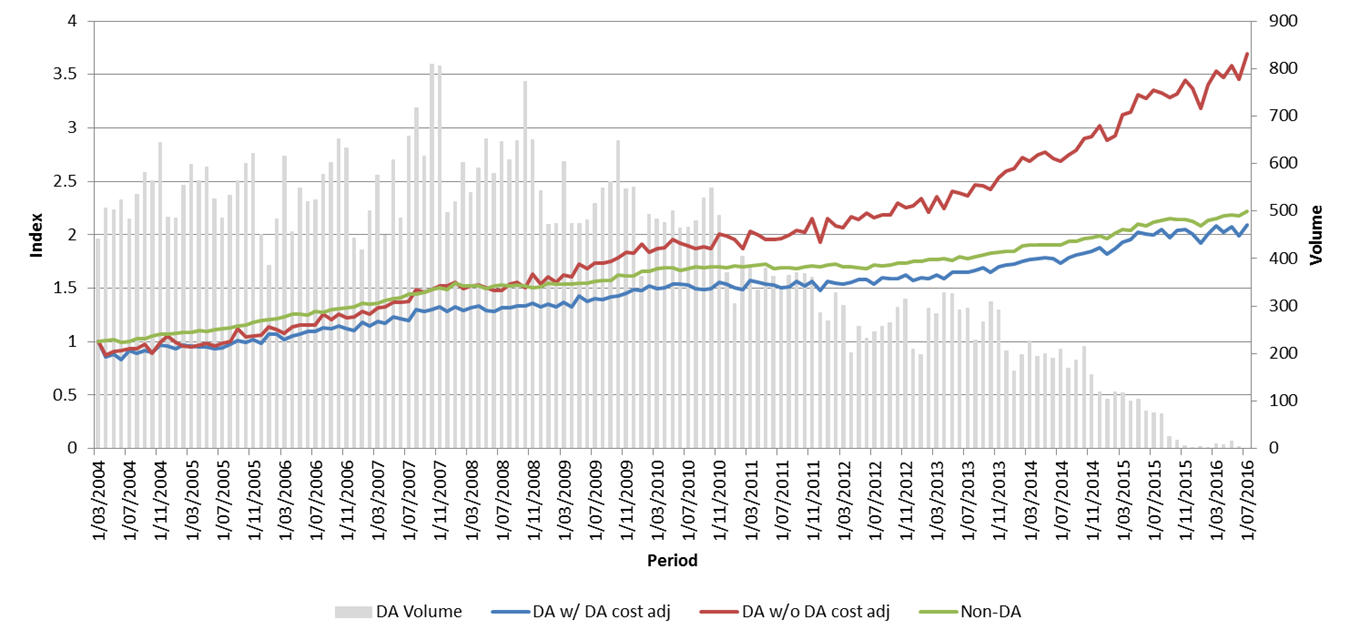
\includegraphics[width=\columnwidth]{Figures/Repeat_sales_index_post_2004_notional_purchase.png}
 \caption{Repeat Sales Index (2004-2016) - DA vs Non-DA}
 \label{fig:BMN_RS_index_post_2004}
\end{figure}

The coefficients $b_j$ on each of the dummies corresponds to the log value of the index. Therefore, we take anti-log of the regression estimates to get the raw index values. Finally, we re-base the index for the starting point - March 2004 to 1 and apply the consecutive period growth rate of the raw index to the current index value, starting from the base period - March 2004.  $\epsilon$ is the random error term in the log form with zero mean and constant variance. The notional purchase price for unimproved homes is the actual purchase price, while the notional purchase price for modified homes is the expected price at the time of DA plus the cost of development. 

%
\begin{figure}[!ht]
    \centering
  %  \textbf{Repeat Sales Index - DA and Non DA}\par\medskip
    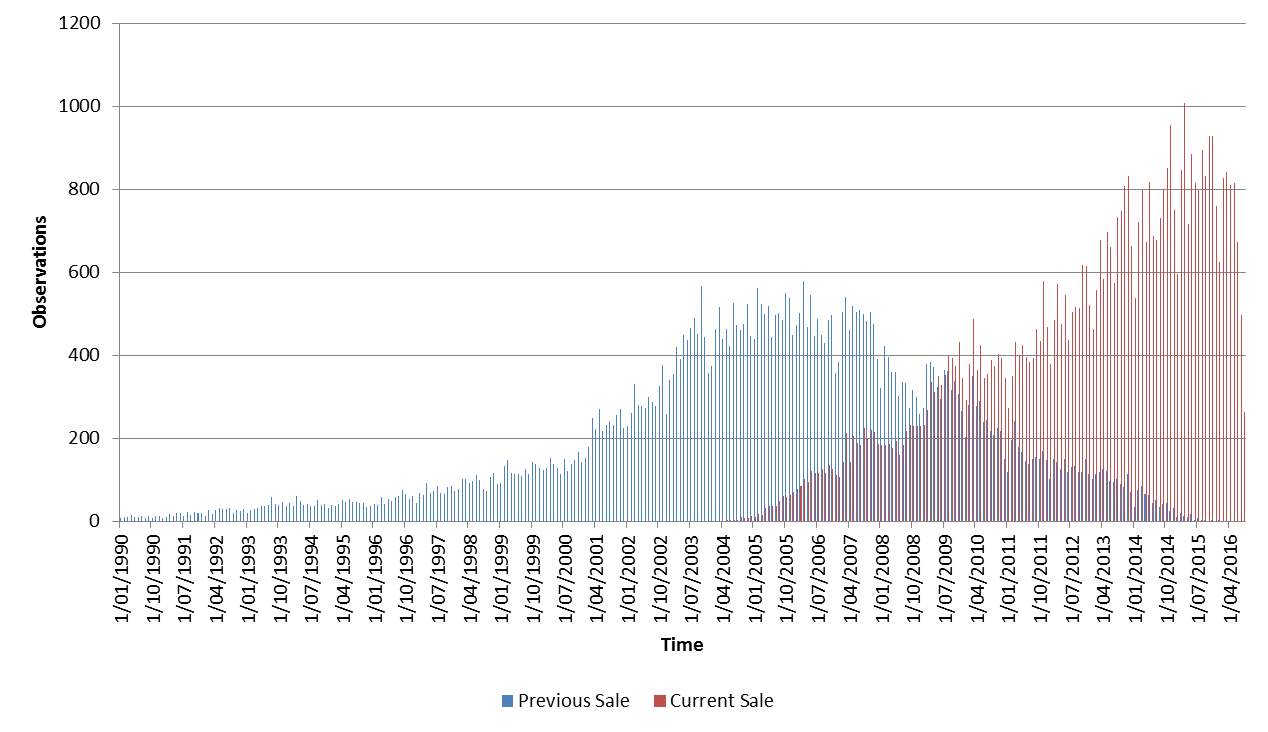
\includegraphics[width=\textwidth]{Figures/prev_cur_sale_dist.png}
    \caption{Repeat Sales Index with DA volumes}
    \label{fig:BMN}
\end{figure}
Figure \ref{fig:BMN_RS_index_post_2004} shows the repeat sales index for unimproved properties and improved properties before and after cost adjustment. The results show that, over time, the house prices for improved properties have appreciated much more than the unimproved properties. However when we account for the improvement spending, the house price appreciation is lower than unimproved homes. So, for example, if both improved and unimproved properties are bought in 2004 and sold any time until 2016, the house prices for improved homes are constantly below unimproved homes. Therefore, over time, the returns, on average, are lower than than the unimproved homes. This is consistent with and confirms our main findings.

Since our data uses only repeat sales records, some of homes that have done improvement may not have sold yet and therefore they do not form part our data set. Hence we see that the home improvement volumes are stable from 2004 to 2010 period and then start to decline. We also see that the repeat sale index before cost adjustment is initially lower than unimproved homes. This is because there are not many observations where properties have have been bought, improved and sold in the initial few years. As the time period increases the number of observations also increase and therefore we start to see more prominent effect after the initial few years where the price appreciate at a faster rate than unimproved homes.

  
\subsection{Location Fixed Effect - Statistical Subdivision Level}

The main model controls for the geographical factors affecting the returns using the state fixed effects. However the house prices could vary significantly even within the state. For example, in NSW, house prices in capital city - Sydney could be considerably higher than prices in rest of the NSW. Since we model the returns, these variations in house prices should cancel out each other. Nonetheless, the geographical factor at lower level than state could still affect variations in the returns. Therefore we test the main results by controlling for the geographical factors at statistical subdivision (SSD) level.

Table \ref{tab:results_ssd} presents results for models 1 to 8 with SSD level location fixed effects. In models 7 and 8, we find that the results are consistent with the main results. The return, at aggregate level, for improved homes is 1.9\% and 2.4\% lower than unimproved homes respectively. 

\newgeometry{margin=1in}
% Table created by stargazer v.5.2 by Marek Hlavac, Harvard University. E-mail: hlavac at fas.harvard.edu
% Date and time: Wed, Jun 14, 2017 - 04:52:42 AM
% Requires LaTeX packages: dcolumn rotating 
\begin{sidewaystable}[!htbp] \centering 
  \caption{Fixed Effects Model Results - SSD Region level} 
  \label{tab:results_ssd}
    \resizebox{\textwidth}{!}{
\begin{threeparttable}

\begin{tabular}{@{\extracolsep{5pt}}lD{.}{.}{-3} D{.}{.}{-3} D{.}{.}{-3} D{.}{.}{-3} D{.}{.}{-3} D{.}{.}{-3} D{.}{.}{-3} D{.}{.}{-3} } 
\\[-1.8ex] 
\toprule \\[-1.8ex] 
\\[-1.8ex] & \multicolumn{8}{c}{Log(Resale Price/Purchase Price (Notional))} \\ 
\\[-1.8ex] & \multicolumn{1}{c}{(1)} & \multicolumn{1}{c}{(2)} & \multicolumn{1}{c}{(3)} & \multicolumn{1}{c}{(4)} & \multicolumn{1}{c}{(5)} & \multicolumn{1}{c}{(6)} & \multicolumn{1}{c}{(7)} & \multicolumn{1}{c}{(8)}\\ 
\midrule \\[-1.8ex] 
 DA &  &  &  &  &  &  & -0.019^{***} & -0.024^{***} \\ 
  &  &  &  &  &  &  & (0.002) & (0.002) \\ 
  %& & & & & & & & \\ 
 Carports/Garages/Sheds & -0.070^{***} & -0.074^{***} & -0.002 & -0.001 & -0.000 & -0.005 &  &  \\ 
  & (0.007) & (0.007) & (0.007) & (0.007) & (0.006) & (0.007) &  &  \\ 
  %& & & & & & & & \\ 
 Duplex & 0.160^{***} & 0.114^{***} & 0.084^{***} & 0.094^{***} & 0.096^{***} & 0.096^{***} &  &  \\ 
  & (0.012) & (0.012) & (0.013) & (0.013) & (0.013) & (0.013) &  &  \\ 
  %& & & & & & & & \\ 
 Extension/Alteration & 0.029^{***} & -0.009^{***} & -0.009^{***} & -0.010^{***} & -0.010^{***} & -0.012^{***} &  &  \\ 
  & (0.003) & (0.003) & (0.004) & (0.004) & (0.004) & (0.004) &  &  \\ 
  %& & & & & & & & \\ 
 House/Single Dwelling & -0.080^{***} & -0.125^{***} & -0.117^{***} & -0.110^{***} & -0.109^{***} & -0.111^{***} &  &  \\ 
  & (0.005) & (0.005) & (0.007) & (0.007) & (0.007) & (0.007) &  &  \\ 
  %& & & & & & & & \\ 
 Multiple DA & 0.034^{***} & -0.005 & -0.023^{***} & -0.015^{**} & -0.015^{**} & -0.021^{***} &  &  \\ 
  & (0.003) & (0.003) & (0.006) & (0.006) & (0.006) & (0.006) &  &  \\ 
  %& & & & & & & & \\ 
 Swimming Pool & 0.189^{***} & 0.156^{***} & 0.002 & 0.007^{**} & 0.007^{**} & -0.002 &  &  \\ 
  & (0.004) & (0.004) & (0.003) & (0.003) & (0.003) & (0.003) &  &  \\ 
  %& & & & & & & & \\ 
 Verandahs/Pergolas & 0.024^{***} & 0.015^{***} & -0.028^{***} & -0.026^{***} & -0.027^{***} & -0.031^{***} &  &  \\ 
  & (0.004) & (0.004) & (0.003) & (0.003) & (0.003) & (0.003) &  &  \\ 
  %& & & & & & & & \\ 
 MktReturn & 0.766^{***} & 0.775^{***} & 0.809^{***} & 0.955^{***} & 0.954^{***} & 0.954^{***} & 0.955^{***} & 0.955^{***} \\ 
  & (0.002) & (0.003) & (0.003) & (0.003) & (0.003) & (0.003) & (0.003) & (0.003) \\ 
  %& & & & & & & & \\ 
 Months between sales &  &  &  & -0.001^{***} & -0.002^{***} & -0.002^{***} & -0.002^{***} & -0.002^{***} \\ 
  &  &  &  & (0.000) & (0.000) & (0.000) & (0.000) & (0.000) \\ 
  %& & & & & & & & \\ 
 Months between sales squared &  &  &  &  & 0.000^{***} & 0.000^{***} & 0.000^{***} & 0.000^{***} \\ 
  &  &  &  &  & (0.000) & (0.000) & (0.000) & (0.000) \\ 
  %& & & & & & & & \\ 
 No. of beds (resale) &  & 0.016^{***} & 0.025^{***} & 0.026^{***} & 0.026^{***} &  & 0.025^{***} &  \\ 
  &  & (0.001) & (0.001) & (0.001) & (0.001) &  & (0.001) &  \\ 
  %& & & & & & & & \\ 
 No. of baths (resale) &  & 0.054^{***} & 0.051^{***} & 0.052^{***} & 0.052^{***} &  & 0.051^{***} &  \\ 
  &  & (0.001) & (0.001) & (0.001) & (0.001) &  & (0.001) &  \\ 
  %& & & & & & & & \\ 
 No. of cars (resale) &  & 0.001^{***} & 0.006^{***} & 0.008^{***} & 0.008^{***} &  & 0.008^{***} &  \\ 
  &  & (0.000) & (0.000) & (0.000) & (0.000) &  & (0.000) &  \\ 
  %& & & & & & & & \\ 
 No. of beds (purchase) &  &  & -0.031^{***} & -0.031^{***} & -0.031^{***} &  & -0.031^{***} &  \\ 
  &  &  & (0.001) & (0.001) & (0.001) &  & (0.001) &  \\ 
  %& & & & & & & & \\ 
 No. of baths (purchase) &  &  & -0.070^{***} & -0.070^{***} & -0.070^{***} &  & -0.069^{***} &  \\ 
  &  &  & (0.001) & (0.001) & (0.001) &  & (0.001) &  \\ 
  %& & & & & & & & \\ 
 No. of cars (purchase) &  &  & -0.013^{***} & -0.014^{***} & -0.014^{***} &  & -0.014^{***} &  \\ 
  &  &  & (0.000) & (0.000) & (0.000) &  & (0.000) &  \\ 
  %& & & & & & & & \\ 
 Change in \# of beds &  &  &  &  &  & 0.028^{***} &  & 0.027^{***} \\ 
  &  &  &  &  &  & (0.001) &  & (0.001) \\ 
  %& & & & & & & & \\ 
 Change in \# of baths &  &  &  &  &  & 0.060^{***} &  & 0.059^{***} \\ 
  &  &  &  &  &  & (0.001) &  & (0.001) \\ 
  %& & & & & & & & \\ 
 Change in \# of cars &  &  &  &  &  & 0.010^{***} &  & 0.010^{***} \\ 
  &  &  &  &  &  & (0.000) &  & (0.000) \\ 
  %& & & & & & & & \\ 
 Constant & 0.148^{***} & 0.023^{***} & 0.160^{***} & 0.179^{***} & 0.194^{***} & 0.143^{***} & 0.193^{***} & 0.144^{***} \\ 
  & (0.004) & (0.006) & (0.006) & (0.006) & (0.006) & (0.006) & (0.006) & (0.006) \\ 
  %& & & & & & & & \\ 
Year Fixed Effects & Yes & Yes & Yes & Yes & Yes & Yes & Yes & Yes \\ 
Location Fixed Effects & Yes & Yes & Yes & Yes & Yes & Yes & Yes & Yes \\ 
Observations & \multicolumn{1}{c}{1,119,293} & \multicolumn{1}{c}{1,012,436} & \multicolumn{1}{c}{517,011} & \multicolumn{1}{c}{517,011} & \multicolumn{1}{c}{517,011} & \multicolumn{1}{c}{517,011} & \multicolumn{1}{c}{517,011} & \multicolumn{1}{c}{517,011} \\ 
Adjusted R$^{2}$ & \multicolumn{1}{c}{0.140} & \multicolumn{1}{c}{0.165} & \multicolumn{1}{c}{0.302} & \multicolumn{1}{c}{0.311} & \multicolumn{1}{c}{0.312} & \multicolumn{1}{c}{0.309} & \multicolumn{1}{c}{0.311} & \multicolumn{1}{c}{0.308} \\ 
%F Statistic & \multicolumn{1}{c}{887.768$^{***}$ (df = 206; 1119086)} & \multicolumn{1}{c}{955.373$^{***}$ (df = 209; 1012226)} & \multicolumn{1}{c}{1,057.003$^{***}$ (df = 212; 516798)} & \multicolumn{1}{c}{1,098.319$^{***}$ (df = 213; 516797)} & \multicolumn{1}{c}{1,096.034$^{***}$ (df = 214; 516796)} & \multicolumn{1}{c}{1,095.434$^{***}$ (df = 211; 516799)} & \multicolumn{1}{c}{1,123.717$^{***}$ (df = 208; 516802)} & \multicolumn{1}{c}{1,123.728$^{***}$ (df = 205; 516805)} \\ 

F Statistic & \multicolumn{1}{c}{887.768$^{***}$} & \multicolumn{1}{c}{955.373$^{***}$} & \multicolumn{1}{c}{1,057.003$^{***}$} & \multicolumn{1}{c}{1,098.319$^{***}$} & \multicolumn{1}{c}{1,096.034$^{***}$} & \multicolumn{1}{c}{1,095.434$^{***}$} & \multicolumn{1}{c}{1,123.717$^{***}$} & \multicolumn{1}{c}{1,123.728$^{***}$} \\ 

& \multicolumn{1}{c}{(df = 206; 1119086)} & \multicolumn{1}{c}{(df = 209; 1012226)} & \multicolumn{1}{c}{(df = 212; 516798)} & \multicolumn{1}{c}{(df = 213; 516797)} & \multicolumn{1}{c}{(df = 214; 516796)} & \multicolumn{1}{c}{(df = 211; 516799)} & \multicolumn{1}{c}{(df = 208; 516802)} & \multicolumn{1}{c}{(df = 205; 516805)} \\ 

\bottomrule \\[-1.8ex] 
%\textit{Notes:} & \multicolumn{8}{l}{Robust standard errors in parentheses. *** 0.1\% significance ** 1\% significance * 5\% significance . 10\% significance} \\

\end{tabular}%

\begin{tablenotes}[para,flushleft]
  \LARGE
      Notes: Robust standard errors are reported in parentheses, Significance of variables is adjusted accordingly. *** 0.1\% significance ** 1\% significance * 5\% significance. We have a total of 1,119,419 (55,733 for treatment and 1,063,686 for control sample) possible observation with deviation accounted for by missing data.
\end{tablenotes}    



\end{threeparttable}
}
\end{sidewaystable} 
\restoregeometry 

When we look at by improvement types, the returns, as per models 1 to 6 are generally consistent with the main results. The coefficient for carports/garages/sheds is mostly insignificant. The returns for duplex is around 9\% higher than unimproved homes which is also consistent with the main results.

For extension/alterations, the returns were insignificant in the main results, however when we control at SSD level location fixed effects, the coefficient becomes significant around -1\%. For House/Single Dwelling, Multiple DAs, swimming pool and verandas/pergolas, the returns are consistent with the main results, around 11\%, 1.5\%, 0.7\% and 2.7\% lower than unimproved homes respectively. We also note that after controlling for location effects at SSD level, the mktReturn variable captures around 95\% of the variation in the returns as compared to 92\% with State level fixed effects.

\subsection{Council Restriction Bias}

In the main model results, our control sample included properties from all the suburbs. However, there could be a few councils that do not disclose development application data and therefore Cordell would not have a record all the homes with development approvals. As a result, our control sample of unimproved homes may incorrectly include some properties that have a development approval and have subsequently carried out home improvements. This could potentially bias our main results, as for those properties, we would have the value of home improvement implicitly accounted for in the resale price while the costs of improvement would be ignored. 

Hence to rule out this bias, we use a self-selection method to identify unbiased control group. At the suburb level, we find all the areas where we have at least one improved home record available and then we take all the unimproved properties from those suburbs only. This way we ensure that all the properties in the control sample are from suburbs where council restriction don't apply. Using this self-selection technique, out of \~1.08m records of unimproved homes, we have around 60,438 records that are excluded from the control sample leaving us with \~1.02m records. 

Table \ref{tab:results_s1} shows the results, based on this control sample and we find that the estimates are robust and consistent with the main results. Full model specification 7 and 8 show that the returns, at aggregate level, for improved homes are 2\% and 2.4\% lower than unimproved homes. Also when we split the returns by improvement types the results are generally consistent with the main results. Return for carports is around 2.1\% lower than unimproved homes. For duplex the return is 9.7\% higher. The return for extension/alteration is insignificantly different from unimproved homes. The coefficient on house single/dwelling is negative 10\%. Multiple DAs has coefficient of -1.2\% (weakly significant). Swimming pool is insignificant and verandas/pergolas has 3.8\% lower returns.

\clearpage
\newgeometry{margin=1in}
% Table created by stargazer v.5.2 by Marek Hlavac, Harvard University. E-mail: hlavac at fas.harvard.edu
% Date and time: Fri, Jun 30, 2017 - 11:26:21 AM
% Requires LaTeX packages: dcolumn rotating 
\begin{sidewaystable}[!htbp] \centering 
  \caption{Sample Coverage} 
  \label{tab:results_s1} 
    \resizebox{\textwidth}{!}{
\begin{tabular}{@{\extracolsep{5pt}}lD{.}{.}{-3} D{.}{.}{-3} D{.}{.}{-3} D{.}{.}{-3} D{.}{.}{-3} D{.}{.}{-3} D{.}{.}{-3} D{.}{.}{-3} } 
\\[-1.8ex] 
\toprule \\[-1.8ex] 
\\[-1.8ex] & \multicolumn{8}{c}{Log(Resale Price/Purchase Price (Notional))} \\ 
\\[-1.8ex] & \multicolumn{1}{c}{(1)} & \multicolumn{1}{c}{(2)} & \multicolumn{1}{c}{(3)} & \multicolumn{1}{c}{(4)} & \multicolumn{1}{c}{(5)} & \multicolumn{1}{c}{(6)} & \multicolumn{1}{c}{(7)} & \multicolumn{1}{c}{(8)}\\ 
\midrule \\[-1.8ex] 
 DA &  &  &  &  &  &  & -0.020^{***} & -0.024^{***} \\ 
  &  &  &  &  &  &  & (0.002) & (0.002) \\ 
  & & & & & & & & \\ 
 Carports/Garages/Sheds & -0.091^{***} & -0.091^{***} & -0.022^{***} & -0.021^{***} & -0.021^{***} & -0.026^{***} &  &  \\ 
  & (0.007) & (0.007) & (0.007) & (0.007) & (0.007) & (0.007) &  &  \\ 
  & & & & & & & & \\ 
 Duplex & 0.179^{***} & 0.134^{***} & 0.093^{***} & 0.096^{***} & 0.097^{***} & 0.100^{***} &  &  \\ 
  & (0.012) & (0.012) & (0.013) & (0.013) & (0.013) & (0.013) &  &  \\ 
  & & & & & & & & \\ 
 Extension/Alteration & 0.026^{***} & -0.015^{***} & 0.000 & -0.000 & -0.001 & -0.002 &  &  \\ 
  & (0.003) & (0.003) & (0.004) & (0.004) & (0.004) & (0.004) &  &  \\ 
  & & & & & & & & \\ 
 House/Single Dwelling & -0.082^{***} & -0.130^{***} & -0.106^{***} & -0.102^{***} & -0.101^{***} & -0.103^{***} &  &  \\ 
  & (0.005) & (0.004) & (0.007) & (0.007) & (0.007) & (0.007) &  &  \\ 
  & & & & & & & & \\ 
 Multiple DA & 0.020^{***} & -0.021^{***} & -0.019^{***} & -0.013^{**} & -0.012^{*} & -0.018^{***} &  &  \\ 
  & (0.003) & (0.003) & (0.006) & (0.006) & (0.006) & (0.006) &  &  \\ 
  & & & & & & & & \\ 
 Swimming Pool & 0.178^{***} & 0.142^{***} & -0.002 & 0.003 & 0.003 & -0.006^{*} &  &  \\ 
  & (0.004) & (0.004) & (0.003) & (0.003) & (0.003) & (0.003) &  &  \\ 
  & & & & & & & & \\ 
 Verandahs/Pergolas & 0.008^{*} & -0.001 & -0.039^{***} & -0.037^{***} & -0.038^{***} & -0.042^{***} &  &  \\ 
  & (0.004) & (0.004) & (0.004) & (0.004) & (0.004) & (0.004) &  &  \\ 
  & & & & & & & & \\ 
 MktReturn & 0.755^{***} & 0.768^{***} & 0.808^{***} & 0.925^{***} & 0.924^{***} & 0.926^{***} & 0.925^{***} & 0.927^{***} \\ 
  & (0.002) & (0.002) & (0.003) & (0.003) & (0.003) & (0.003) & (0.003) & (0.003) \\ 
  & & & & & & & & \\ 
 Months between sales &  &  &  & -0.001^{***} & -0.002^{***} & -0.002^{***} & -0.002^{***} & -0.002^{***} \\ 
  &  &  &  & (0.000) & (0.000) & (0.000) & (0.000) & (0.000) \\ 
  & & & & & & & & \\ 
 Months between sales squared &  &  &  &  & 0.000^{***} & 0.000^{***} & 0.000^{***} & 0.000^{***} \\ 
  &  &  &  &  & (0.000) & (0.000) & (0.000) & (0.000) \\ 
  & & & & & & & & \\ 
 No. of beds (resale) &  & 0.018^{***} & 0.026^{***} & 0.027^{***} & 0.027^{***} &  & 0.026^{***} &  \\ 
  &  & (0.001) & (0.001) & (0.001) & (0.001) &  & (0.001) &  \\ 
  & & & & & & & & \\ 
 No. of baths (resale) &  & 0.050^{***} & 0.058^{***} & 0.060^{***} & 0.060^{***} &  & 0.059^{***} &  \\ 
  &  & (0.001) & (0.001) & (0.001) & (0.001) &  & (0.001) &  \\ 
  & & & & & & & & \\ 
 No. of cars (resale) &  & 0.001^{**} & 0.004^{***} & 0.006^{***} & 0.006^{***} &  & 0.006^{***} &  \\ 
  &  & (0.000) & (0.000) & (0.000) & (0.000) &  & (0.000) &  \\ 
  & & & & & & & & \\ 
 No. of beds (purchase) &  &  & -0.032^{***} & -0.033^{***} & -0.033^{***} &  & -0.032^{***} &  \\ 
  &  &  & (0.001) & (0.001) & (0.001) &  & (0.001) &  \\ 
  & & & & & & & & \\ 
 No. of baths (purchase) &  &  & -0.069^{***} & -0.069^{***} & -0.069^{***} &  & -0.069^{***} &  \\ 
  &  &  & (0.001) & (0.001) & (0.001) &  & (0.001) &  \\ 
  & & & & & & & & \\ 
 No. of cars (purchase) &  &  & -0.015^{***} & -0.016^{***} & -0.016^{***} &  & -0.016^{***} &  \\ 
  &  &  & (0.000) & (0.000) & (0.000) &  & (0.000) &  \\ 
  & & & & & & & & \\ 
 Change in \# of beds &  &  &  &  &  & 0.029^{***} &  & 0.029^{***} \\ 
  &  &  &  &  &  & (0.001) &  & (0.001) \\ 
  & & & & & & & & \\ 
 Change in \# of baths &  &  &  &  &  & 0.063^{***} &  & 0.063^{***} \\ 
  &  &  &  &  &  & (0.001) &  & (0.001) \\ 
  & & & & & & & & \\ 
 Change in \# of cars &  &  &  &  &  & 0.010^{***} &  & 0.010^{***} \\ 
  &  &  &  &  &  & (0.000) &  & (0.000) \\ 
  & & & & & & & & \\ 
 Constant & 0.103^{***} & -0.024^{**} & 0.096^{***} & 0.127^{***} & 0.142^{***} & 0.093^{***} & 0.142^{***} & 0.093^{***} \\ 
  & (0.011) & (0.012) & (0.012) & (0.012) & (0.012) & (0.012) & (0.012) & (0.012) \\ 
  & & & & & & & & \\ 
Year Fixed Effects & Yes & Yes & Yes & Yes & Yes & Yes & Yes &  \\ 
Location Fixed Effects & Yes & Yes & Yes & Yes & Yes & Yes & Yes &  \\ 
Observations & \multicolumn{1}{c}{1,085,083} & \multicolumn{1}{c}{985,860} & \multicolumn{1}{c}{508,235} & \multicolumn{1}{c}{508,235} & \multicolumn{1}{c}{508,235} & \multicolumn{1}{c}{508,235} & \multicolumn{1}{c}{508,235} & \multicolumn{1}{c}{508,235} \\ 
Adjusted R$^{2}$ & \multicolumn{1}{c}{0.128} & \multicolumn{1}{c}{0.152} & \multicolumn{1}{c}{0.285} & \multicolumn{1}{c}{0.293} & \multicolumn{1}{c}{0.293} & \multicolumn{1}{c}{0.291} & \multicolumn{1}{c}{0.293} & \multicolumn{1}{c}{0.290} \\ 
F Statistic & \multicolumn{1}{c}{5,903.084$^{***}$ (df = 27; 1085055)} & \multicolumn{1}{c}{5,888.807$^{***}$ (df = 30; 985829)} & \multicolumn{1}{c}{6,137.642$^{***}$ (df = 33; 508201)} & \multicolumn{1}{c}{6,190.773$^{***}$ (df = 34; 508200)} & \multicolumn{1}{c}{6,030.919$^{***}$ (df = 35; 508199)} & \multicolumn{1}{c}{6,517.130$^{***}$ (df = 32; 508202)} & \multicolumn{1}{c}{7,253.018$^{***}$ (df = 29; 508205)} & \multicolumn{1}{c}{7,993.324$^{***}$ (df = 26; 508208)} \\ 
\bottomrule \\[-1.8ex] 
\textit{Notes:} & \multicolumn{8}{l}{Robust standard errors in parentheses. *** 0.1\% significance ** 1\% significance * 5\% significance . 10\% significance} \\ 
\end{tabular} 
}
\end{sidewaystable} 
\restoregeometry

\clearpage
\newgeometry{margin=1in}
% Table created by stargazer v.5.2 by Marek Hlavac, Harvard University. E-mail: hlavac at fas.harvard.edu
% Date and time: Fri, Jun 30, 2017 - 11:11:20 AM
% Requires LaTeX packages: dcolumn rotating 
\begin{sidewaystable}[!htbp] \centering 
  \caption{Including Improved Homes Purchased Post 2004} 
  \label{tab:result_s1_prev2004} 
  \resizebox{\textwidth}{!}{
\begin{threeparttable}

\begin{tabular}{@{\extracolsep{5pt}}lD{.}{.}{-3} D{.}{.}{-3} D{.}{.}{-3} D{.}{.}{-3} D{.}{.}{-3} D{.}{.}{-3} } 
\\[-1.8ex] 
\toprule \\[-1.8ex] 
\\[-1.8ex] & \multicolumn{6}{c}{Log(Resale Price/Purchase Price (Notional))} \\ 
\\[-1.8ex] & \multicolumn{1}{c}{(1)} & \multicolumn{1}{c}{(2)} & \multicolumn{1}{c}{(3)} & \multicolumn{1}{c}{(4)} & \multicolumn{1}{c}{(5)} & \multicolumn{1}{c}{(6)}\\ 
\midrule \\[-1.8ex] 
 DA &  &  &  &  & -0.018^{***} & -0.022^{***} \\ 
  &  &  &  &  & (0.002) & (0.002) \\ 
  %& & & & & & \\ 
 Carports/Garages/Sheds & -0.020^{***} & -0.020^{***} & -0.019^{***} & -0.024^{***} &  &  \\ 
  & (0.007) & (0.007) & (0.007) & (0.007) &  &  \\ 
  %& & & & & & \\ 
 Duplex & 0.090^{***} & 0.091^{***} & 0.093^{***} & 0.095^{***} &  &  \\ 
  & (0.014) & (0.014) & (0.014) & (0.014) &  &  \\ 
  %& & & & & & \\ 
 Extension/Alteration & 0.008^{**} & 0.006 & 0.005 & 0.004 &  &  \\ 
  & (0.004) & (0.004) & (0.004) & (0.004) &  &  \\ 
  %& & & & & & \\ 
 House/Single Dwelling & -0.106^{***} & -0.102^{***} & -0.101^{***} & -0.103^{***} &  &  \\ 
  & (0.007) & (0.007) & (0.007) & (0.007) &  &  \\ 
  %& & & & & & \\ 
 Multiple DA & -0.013^{*} & -0.008 & -0.008 & -0.014^{**} &  &  \\ 
  & (0.007) & (0.007) & (0.007) & (0.007) &  &  \\ 
  %& & & & & & \\ 
 Swimming Pool & -0.003 & 0.001 & 0.002 & -0.008^{**} &  &  \\ 
  & (0.004) & (0.004) & (0.004) & (0.004) &  &  \\ 
  %& & & & & & \\ 
 Verandahs/Pergolas & -0.032^{***} & -0.031^{***} & -0.032^{***} & -0.036^{***} &  &  \\ 
  & (0.004) & (0.004) & (0.004) & (0.004) &  &  \\ 
  %& & & & & & \\ 
 MktReturn & 0.808^{***} & 0.926^{***} & 0.926^{***} & 0.927^{***} & 0.926^{***} & 0.928^{***} \\ 
  & (0.003) & (0.003) & (0.003) & (0.003) & (0.003) & (0.003) \\ 
  %& & & & & & \\ 
 Months between sales &  & -0.001^{***} & -0.002^{***} & -0.002^{***} & -0.002^{***} & -0.002^{***} \\ 
  &  & (0.000) & (0.000) & (0.000) & (0.000) & (0.000) \\ 
  %& & & & & & \\ 
 Months between sales squared &  &  & 0.000^{***} & 0.000^{***} & 0.000^{***} & 0.000^{***} \\ 
  &  &  & (0.000) & (0.000) & (0.000) & (0.000) \\ 
  %& & & & & & \\ 
 No. of beds (resale) & 0.026^{***} & 0.027^{***} & 0.027^{***} &  & 0.026^{***} &  \\ 
  & (0.001) & (0.001) & (0.001) &  & (0.001) &  \\ 
  %& & & & & & \\ 
 No. of baths (resale) & 0.058^{***} & 0.059^{***} & 0.059^{***} &  & 0.059^{***} &  \\ 
  & (0.001) & (0.001) & (0.001) &  & (0.001) &  \\ 
  %& & & & & & \\ 
 No. of cars (resale) & 0.004^{***} & 0.006^{***} & 0.006^{***} &  & 0.006^{***} &  \\ 
  & (0.000) & (0.000) & (0.000) &  & (0.000) &  \\ 
  %& & & & & & \\ 
 No. of beds (purchase) & -0.032^{***} & -0.033^{***} & -0.033^{***} &  & -0.032^{***} &  \\ 
  & (0.001) & (0.001) & (0.001) &  & (0.001) &  \\ 
  %& & & & & & \\ 
 No. of baths (purchase) & -0.069^{***} & -0.069^{***} & -0.069^{***} &  & -0.068^{***} &  \\ 
  & (0.001) & (0.001) & (0.001) &  & (0.001) &  \\ 
  %& & & & & & \\ 
 No. of cars (purchase) & -0.015^{***} & -0.016^{***} & -0.016^{***} &  & -0.016^{***} &  \\ 
  & (0.000) & (0.000) & (0.000) &  & (0.000) &  \\ 
  %& & & & & & \\ 
 Change in \# of beds &  &  &  & 0.029^{***} &  & 0.029^{***} \\ 
  &  &  &  & (0.001) &  & (0.001) \\ 
  %& & & & & & \\ 
 Change in \# of baths &  &  &  & 0.063^{***} &  & 0.063^{***} \\ 
  &  &  &  & (0.001) &  & (0.001) \\ 
  %& & & & & & \\ 
 Change in \# of cars &  &  &  & 0.010^{***} &  & 0.010^{***} \\ 
  &  &  &  & (0.000) &  & (0.000) \\ 
  %& & & & & & \\ 
 Constant & 0.086^{***} & 0.111^{***} & 0.127^{***} & 0.076^{***} & 0.127^{***} & 0.076^{***} \\ 
  & (0.002) & (0.002) & (0.003) & (0.002) & (0.003) & (0.002) \\ 
  %& & & & & & \\ 
Year Fixed Effects & Yes & Yes & Yes & Yes & Yes & Yes \\ 
Location Fixed Effects & Yes & Yes & Yes & Yes & Yes & Yes \\ 
Observations & \multicolumn{1}{c}{504,893} & \multicolumn{1}{c}{504,893} & \multicolumn{1}{c}{504,893} & \multicolumn{1}{c}{504,893} & \multicolumn{1}{c}{504,893} & \multicolumn{1}{c}{504,893} \\ 
Adjusted R$^{2}$ & \multicolumn{1}{c}{0.284} & \multicolumn{1}{c}{0.292} & \multicolumn{1}{c}{0.292} & \multicolumn{1}{c}{0.290} & \multicolumn{1}{c}{0.292} & \multicolumn{1}{c}{0.289} \\ 
F Statistic & \multicolumn{1}{c}{6,452.740$^{***}$ (df = 31; 504861)} & \multicolumn{1}{c}{6,498.731$^{***}$ (df = 32; 504860)} & \multicolumn{1}{c}{6,320.072$^{***}$ (df = 33; 504859)} & \multicolumn{1}{c}{6,867.966$^{***}$ (df = 30; 504862)} & \multicolumn{1}{c}{7,699.735$^{***}$ (df = 27; 504865)} & \multicolumn{1}{c}{8,557.664$^{***}$ (df = 24; 504868)} \\ 



\bottomrule \\[-1.8ex] 

\end{tabular} 

\begin{tablenotes}[para,flushleft]
  \LARGE
      Notes: Robust standard errors are reported in parentheses, Significance of variables is adjusted accordingly. *** 0.1\% significance ** 1\% significance * 5\% significance. We have a total of 1,064,462 (36,894 for treatment and 1,027,568 for control sample) possible observation with deviation accounted for by missing data.
\end{tablenotes}    



\end{threeparttable}
}
\end{sidewaystable} 
\restoregeometry

\subsection{Including Improved Homes Post 2004}

Since Cordell has data on development approvals available from 2004 onward, we cannot identify if the properties were improved or not prior 2004. Therefore for the reference group - unimproved homes, we take homes purchased post 2004 only. For treatment group however, we take properties purchased post 1990. Also since these are classified as improved homes, there will be relatively a smaller portion of properties that may have carried out additional improvement prior 2004. Any value attributed to the improvement prior 2004 will be implicit in the resale price but the improvement cost prior 2004, would not have been accounted for and therefore, in aggregate, the cost of development for improved homes would be underestimated for such properties only and, in aggregate, make the estimates even more negative. Therefore it does not affect our main analysis adversely. Also, in the interest of having a reasonable sample size, we take all the properties in the main analysis.

However, as part of robustness, we test the results to ensure that the estimates are consistent and stable by excluding the homes purchased prior 2004 for improved homes as well. To make the model more robust, we also exclude the properties from the reference that may induce council restriction bias. Table \ref{tab:result_s1_prev2004} shows the results after excluding improved homes that were bought before 2004. We find that the results are all consistent with the main results.

\clearpage
\subsection{Return of Improved Homes for Investors by no. of years between sales}

In further analysis, we find that the returns for type I investors is higher for improved homes when we classify the investor as time between purchase and resale less than 2 years. In figure \ref{fig:relative_returns_by_investor}, we plot the estimates profile for returns on improved homes relative to unimproved homes by filtering data for each of the groups i.e. from less than 2 years up to less than 24 years. 

\begin{figure}[!ht]
    \centering
     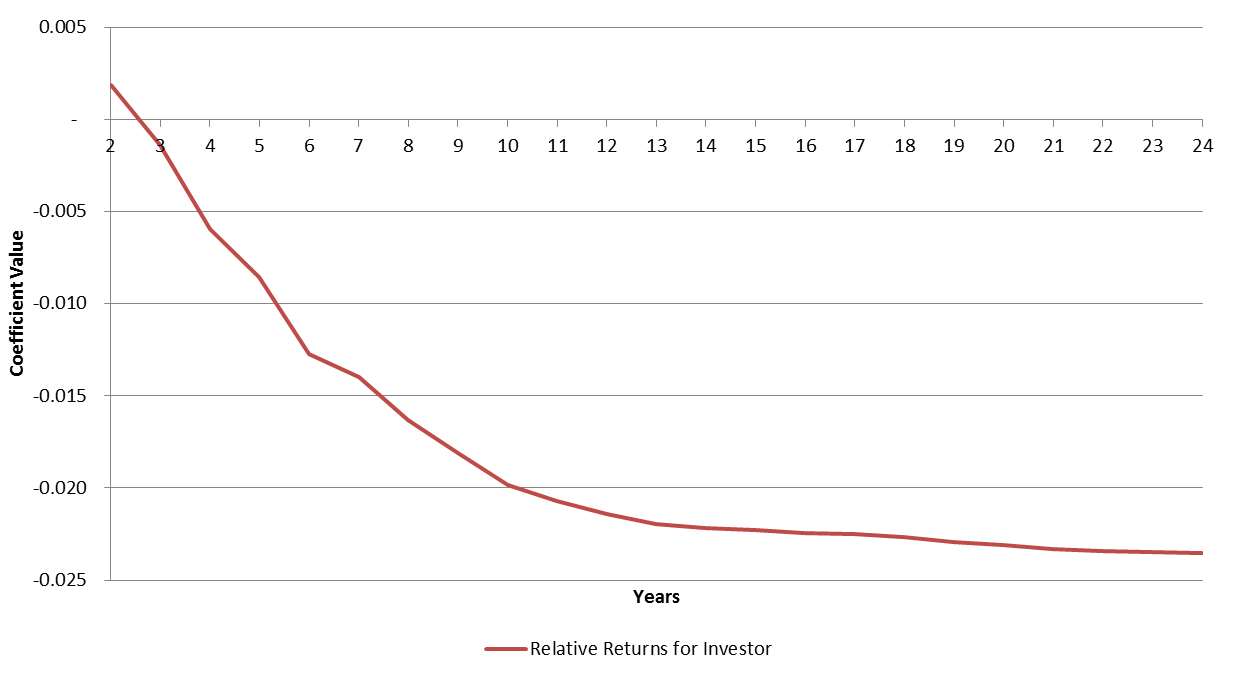
\includegraphics[width=0.9\columnwidth]{Figures/relative_returns_by_investor.png} \par
 \caption{Estimates for Investors classified by no. of years between sales}
 \label{fig:relative_returns_by_investor}
\end{figure}


We see that for less than 2 years i.e. for the investor type I, the returns are positive and as we increase the period between purchase and resale there are more homeowners, included in the regression, who are probably owner occupiers and unlikely to have investment motive at the onset. Therefore, we see that the returns start to become negative relative to unimproved homes. As we increase the number of years between sales further, the estimates stabilize and converge to the overall mean. 



\subsection{SSD Index Validation}

To calculate the expected house price at the time of development approval, we use the statistical subdivision level house price index as provided by CoreLogic. Since all the properties have sales prices observed at least twice, we leverage the repeat sales information, to test whether the house price index is a good predictor of the market appreciation. We calculate the expected house price at time resale i.e at t = +1 and then calculate the percent prediction errors as $E(P_{+1})/P_{+1} - 1) * 100$. Finally, we plot the density, cumulative density function, QQ and PP plots of percent prediction errors as shown in the figure \ref{fig:Rplot_ssd_err_10}. 

\begin{figure}[!htb]
    \centering
     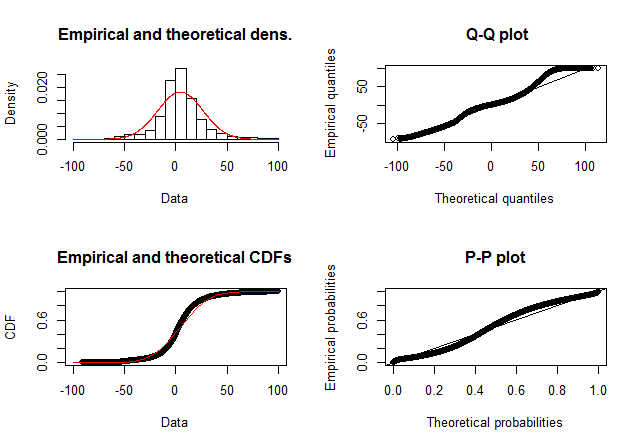
\includegraphics[width=\columnwidth]{Figures/Rplot_qqplot.png} \par
 \caption{House Price Index Prediction Error Distribution}
 \label{fig:Rplot_ssd_err_10}
\end{figure}

We see that the percent prediction error has a symmetric distribution around the mean and is heavily centered around zero. The bell shaped curve represents the normal distribution. The cumulative density fits the normal density. Also in the QQ plot and PP plot, the densities are similar to theoretical densities.


\section{Conclusion}

This paper explores and compares an important economic decision faced by homeowners on the returns of improved homes relative to the unimproved homes. Using a combined data set of house prices and development applications, we test if the returns for improved home is better than unimproved homes. We find that the returns for improved homes, in aggregate, is lower than unimproved homes by around 2.4\%. If we split by improvement types, we find that the highest loss is in building a new house/single dwelling with around 10\% lower returns than unimproved homes. This is mainly attributed to the opportunity cost of lost building value. Carports/Garages/Sheds has around 2.5\% lower returns while verandas/pergolas has around 4.2\% lower return. The return on extension/alteration and swimming pool is not significantly different from unimproved homes. For Duplex, the returns are higher than the unimproved homes by around 10\% and this is due to the double equity generated from the land-split.

In a further analysis, we also examine how the returns compare for the two types of investors and the owner occupiers who buy for their own personal living. Type I investors are classified as those who buy and sell within two years and type II are those homeowners who buy and sell in more than 2 years but invest at some later point to improve their homes and then sell within two years of home improvement. We used an interaction variable between investor and DA dummies and at aggregate level, we find that the returns for improved homes for type I investors are higher than unimproved homes by around 0.4\%. The positive change in the main result is much more prominent in the extension/alteration - around 5.4\% higher than the unimproved homes compared to the insignificant returns in the main results. This explains why typically investors mainly would perform extension/alterations as part of their investment strategy. The returns on carports and verandas/pergolas has also improved from negative to being insignificant. 

In contrast, for type II investors, in aggregate, we find that the returns for improved homes are lower than the unimproved homes by around 1.2\%. When we condition on data, where time between improvement and resale is less than 2 years and split by improvement type, we see that the returns across improvement types have reduced as compared to the main result. This is because the reference category - unimproved homes in both the analysis - investor type I and investor type II, is conditioned by the time between purchase and resale as less than 2 years. Therefore, since, the return for investor group in the reference category - unimproved homes, on average, higher than the non-investor group, the returns on improved homes are even lower. The return on Duplex is reduced from around 10\% to 5.5\%. The return on Extension/alteration has gone from being insignificant to negative 3\%. The returns on house is reduced further to around 22\%. Verandas/Pergolas also reduced to 7\% lower returns. 

So overall this suggests, that homeowner with investment motive who bought and sold the property in less than 2 years have higher returns from home improvements while those home owners who owned the property for more than 2 years but carried out home improvements less than 2 years from selling the property did not make higher returns. So this suggests that the time between sales is the key variable that enables identification of homeowners with investment motive. And homeowners who have investment motive make higher returns and those who are non-investors have lower returns. 

This can be attributed to several factors - since these homeowners have owned the property for relatively longer period (a) They have consumed relatively more value of being able to reside in the property in the form of rental component that is attributed to the housing service. (b) depreciation - homeowners have also relatively consumed more non-durable consumption component in the form of wear and tear of the building. (c) Finally, they also enjoy the profits from house price appreciation mainly attributed to the land value and therefore at the time of resale, they are more psychologically willing to settle for reduced profits.
(d) Finally, they are operating in the long run and therefore they are less likely to have an investment motive right at the beginning i.e. at the time of purchase and hence their choices and decisions are more guided by the social benefits rather than the financial returns. For example, a rational investor would probably add a smaller bedroom or bathroom as there is diminishing returns to housing, whereas the owner occupier would choose the size of the bedroom/bathroom based on his desires and affordability. Therefore, an investor would have make more financial gain, while, owner occupiers, on the other hand consume the non-monetary benefits and probably the relative loss that we estimate in our results is the cost of social benefits that non-investors consume. In a simplistic sense our, paper models and explores the returns on two basic options - do nothing or improve. However, the homeowners may also face another option and that is - switching to a new desired home. Comparing the returns between improving or switching could be an avenue for future research.



\begin{comment}



Also when we look at the estimates profile for investor classified by groups - time between purchase, there is a consistent pattern. The returns are positive returns when the the time between purchase and resale is less than 2 years and as the period increases to less than 3 years and more, the homeowners are less likely to have investment motive and the returns decline initially and then gradually stabilize to the overall mean



if we note that there is no differnce in in returns between type i and type II investor in duplex and house/single dwelling. A major attribution of profits from Duplex would come from double equtiy generated from land split which shoudl be same for bopth groups, likewise a major attribution of losses in houses is from destroyed residual value and these attribution will remain the same acrross investor groups. and that explains why these coefficient are stable in all groups..

you would make money irepsective of being type i ivnestor or type 2 or owner occupier.

So why is it that the investors are making more money...by splitting group by 2 year odf buy and sell, we are able to reasinablly separte the group of homeonwers who would have investment motive right at the time of purchase. and therefore their choices or or decisions would be affected accordingly. For example  children and family..

if homeowner buy and sell within 2 years time, then they are most likely to have an investment motive right at the begining. Due this investment motive the choices, decision and preferences are affected and significantly vary from those owner occupier home owners. For example, an investor, wuld invest in an area where there is likely appreication due. whereas an owner occupier may want to buy the house depending on the distnace to his workplace. this is the part of the reason that affect the return. 







\end{comment}








\begin{comment}


 
Before considering the impact of different type of developments on economic outcomes, we find that households are on average, over capitalized on their investments in the long run. This may be the key signal to potential investors. Table diff in diff shows that the house price is strongly negatively correlated with the post treatment dummy indicating the appreciation rates are lower for properties with DA than with non DA



Yes, the results are quite interesting and it turns out to be in line with our model results as well. I have added the volumes for DA in Fig -1 and provided the previous and current sales volumes distribution in fig 2.
Based on our DA data, we see from the figure 1 below there is a lot of DA activity around 2004 -2010 period. 
The current sales volumes in 2nd figure shows that the current sales (distribution on the right) have increasing volumes from 2005 - 2016 period, and given that the value of the DA will only be captured at the point of repeat sale, we only start to see the effect of DA value in the recent years with prices for DA homes, before adjusting for cost, crossing over the the non da properties around 2012-2013. But after accounting for the DA cost, the da home prices are still below the Non-DA.
A possible reason, why DA home prices remain below non DA prior 2004 (we only have a handfull of observations from 2000 - 2004) is because the DA homes on average may be of poorer quality than non-DA homes anyways. Also DA home prices remain below non-DA from 2004 - 2013 is probably due to the fact that there are not enough observations for DA in earlier periods and as a result we do not have enough repeat (current) sales observations during 2004 - 2013 period. 
So as more and more repeat sales are observerd in the recent years for DA properties, the effect of DA on home prices w/ and w/o cost adjustment as compared to non-DA homes becomes more apparent and prominent.
To rule out the sample selection bias due to the fact that properties may have carried out DA prior 2004 and it is not observed in our data, we can argue as 
case a.   If the DA occurred before the previous sale then it does not matter to our analysis as we would have capture the repeat sale with right returns.
For case b     when DA occured after the previuos sale then we would have captured the prices increase due to DA in the current sale as it is observerd. but we wouldn't have accounted for the DA cost. so as a a robustness check, I did a regression of the mark up model where I only take repeat sales where previous sale is from 2004 onwards, this allows me to ensure that I have properties with right classification of DA or non DA, and that we have accounted for the da cost where applicable. The results from regression, as in table 1 below, indicate that the coefficient of interest is still stable at 0.85.
Also, I can run a robustness check in the DID model too. I can create a dummy for two phases prior 2004 and post 2004 and I can allow for the interaction term to vary for over the phases and check if the coefficient is compares for the entire period 1990 - 2016 with post 2004 phase. 




\begin{figure}[!ht]
    \centering
  %  \textbf{Repeat Sales Index - DA and Non DA}\par\medskip
    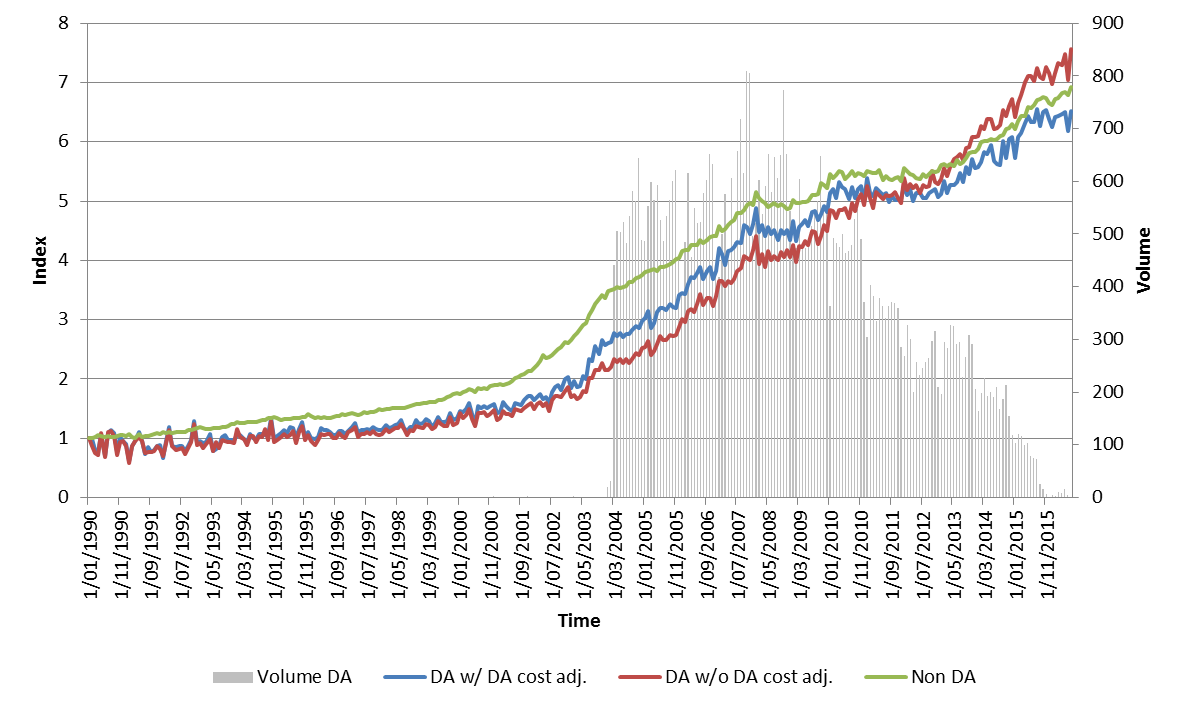
\includegraphics[width=\textwidth]{Figures/cs_rs_index.png}
    \caption{CS Repeat Sales Index with DA volumes}
    \label{fig:BMN}
\end{figure}




%\end{comment}



\subsection{Difference-in-difference method and results}



These results make sense \cite{Einstein05}  properties with re-investments seem to have lower return than the those with no developments. Since housing re-investments are main instruments for house flippers, this finding is compelling. Our next tasks are to check the robustness of these findings to a number of other specifications and to look at the appreciation rates for different building types.


  
  library(AER)
  library(lmtest)
  m <- ivreg(markup ~ value_index_cur_sale_sum + age_da_min + contract_date + max_beds_cur + max_baths_cur + max_cars_cur + max_beds_prev + max_baths_prev + max_cars_prev + building_type_compact2 + state  | area + age_da_min + contract_date + max_beds_cur + max_baths_cur + max_cars_cur + max_beds_prev + max_baths_prev + max_cars_prev + building_type_compact2 + state , data = subset(da_rs_final_duplex_139k, group1 == 'A' & vacant_b_max ==0 & vacant_s_max ==0 & vacant_bs_max ==0 & duplex==0))
  ummary(m, vcov = sandwich, diagnostics = TRUE)


\end{comment}


\bibliographystyle{aer}
\bibliography{sample}


\appendix

\clearpage
\section{Appendix A}

\begin{figure}[!h]
    \centering
     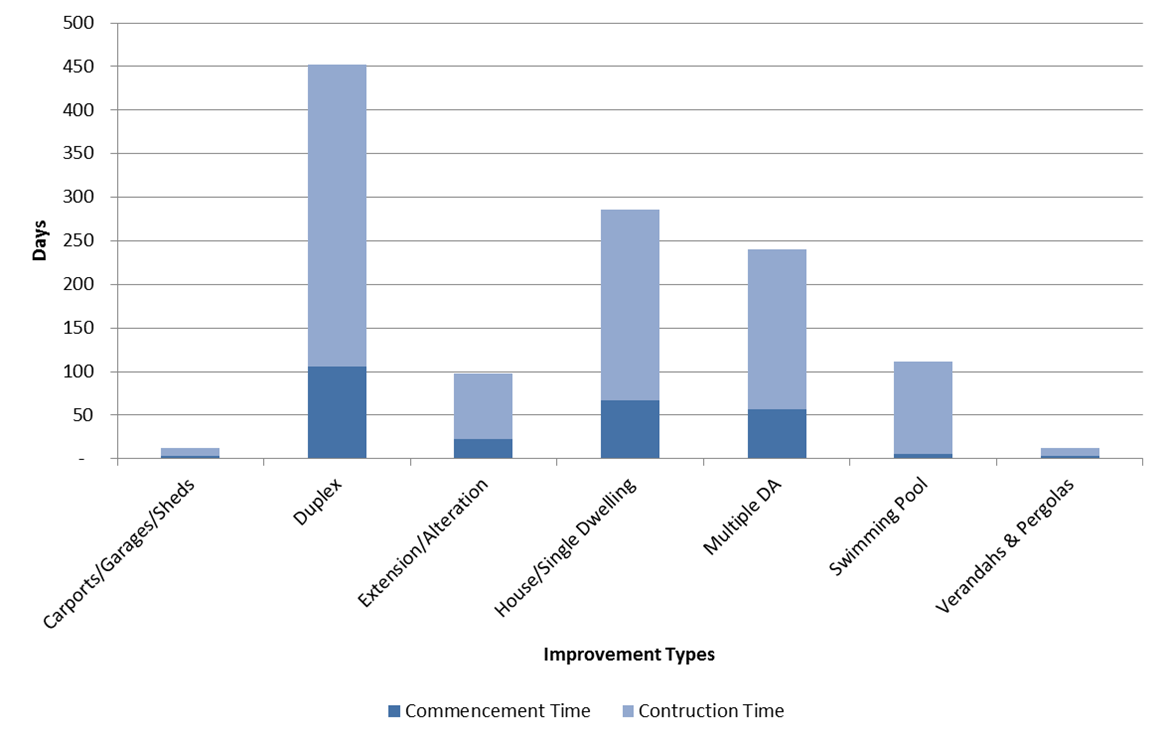
\includegraphics[width=\columnwidth]{Figures/Cm_ct_times.png} \par
 \caption{Average Commencement and Construction times (Days)}
 \label{fig:Cm_ct_times}
\end{figure}




%% Table created by stargazer v.5.2 by Marek Hlavac, Harvard University. E-mail: hlavac at fas.harvard.edu
% Date and time: Wed, Jun 14, 2017 - 04:16:13 AM
% Requires LaTeX packages: dcolumn rotating 
\begin{sidewaystable}[!htbp] \centering
  \caption{Fixed Effect Model Results - DA only sample} 
  \label{results_DA_only_sample} 
    \resizebox{0.9\textwidth}{!}{
\begin{tabular}{@{\extracolsep{5pt}}lD{.}{.}{-3} D{.}{.}{-3} D{.}{.}{-3} D{.}{.}{-3} D{.}{.}{-3} } 
\\[-1.8ex] 
\toprule \\[-1.8ex] 
\\[-1.8ex] & \multicolumn{5}{c}{Log(Resale Price/Purchase Price (Notional))} \\ 
\\[-1.8ex] & \multicolumn{1}{c}{(1)} & \multicolumn{1}{c}{(2)} & \multicolumn{1}{c}{(3)} & \multicolumn{1}{c}{(4)} & \multicolumn{1}{c}{(5)}\\ 
\midrule \\[-1.8ex] 
 Carports/Garages/Sheds & 0.029 & -0.193^{***} & -0.037 & -0.040 & -0.102 \\ 
  & (0.068) & (0.069) & (0.112) & (0.112) & (0.113) \\ 
  & & & & & \\ 
 Duplex & 0.271^{***} & 0.012 & 0.043 & 0.038 & -0.018 \\ 
  & (0.068) & (0.070) & (0.113) & (0.113) & (0.114) \\ 
  & & & & & \\ 
 Extension/Alteration & 0.102 & -0.156^{**} & -0.052 & -0.054 & -0.110 \\ 
  & (0.067) & (0.068) & (0.112) & (0.112) & (0.113) \\ 
  & & & & & \\ 
 House/Single Dwelling & 0.009 & -0.264^{***} & -0.169 & -0.171 & -0.227^{**} \\ 
  & (0.068) & (0.069) & (0.113) & (0.112) & (0.113) \\ 
  & & & & & \\ 
 Multiple DA & 0.122^{*} & -0.149^{**} & -0.058 & -0.061 & -0.121 \\ 
  & (0.068) & (0.069) & (0.113) & (0.112) & (0.113) \\ 
  & & & & & \\ 
 Swimming Pool & 0.257^{***} & 0.001 & -0.023 & -0.024 & -0.087 \\ 
  & (0.068) & (0.069) & (0.112) & (0.112) & (0.113) \\ 
  & & & & & \\ 
 Verandahs/Pergolas & 0.119^{*} & -0.107 & -0.039 & -0.042 & -0.102 \\ 
  & (0.068) & (0.069) & (0.112) & (0.112) & (0.113) \\ 
  & & & & & \\ 
 MktReturn & 0.900^{***} & 0.891^{***} & 0.801^{***} & 0.839^{***} & 0.839^{***} \\ 
  & (0.010) & (0.010) & (0.012) & (0.016) & (0.016) \\ 
  & & & & & \\ 
 Months between sales &  &  &  & -0.000 & -0.000 \\ 
  &  &  &  & (0.000) & (0.000) \\ 
  & & & & & \\ 
 Months between sales squared &  &  &  & -0.000 & -0.000 \\ 
  &  &  &  & (0.000) & (0.000) \\ 
  & & & & & \\ 
 No. of beds (resale) &  & 0.019^{***} & 0.028^{***} & 0.028^{***} &  \\ 
  &  & (0.002) & (0.003) & (0.003) &  \\ 
  & & & & & \\ 
 No. of baths (resale) &  & 0.073^{***} & 0.086^{***} & 0.086^{***} &  \\ 
  &  & (0.003) & (0.003) & (0.003) &  \\ 
  & & & & & \\ 
 No. of cars (resale) &  & 0.013^{***} & 0.011^{***} & 0.011^{***} &  \\ 
  &  & (0.002) & (0.002) & (0.002) &  \\ 
  & & & & & \\ 
 No. of beds (purchase) &  &  & -0.042^{***} & -0.042^{***} &  \\ 
  &  &  & (0.003) & (0.003) &  \\ 
  & & & & & \\ 
 No. of baths (purchase) &  &  & -0.077^{***} & -0.077^{***} &  \\ 
  &  &  & (0.004) & (0.004) &  \\ 
  & & & & & \\ 
 No. of cars (purchase) &  &  & -0.023^{***} & -0.023^{***} &  \\ 
  &  &  & (0.002) & (0.002) &  \\ 
  & & & & & \\ 
 Change in no. of beds &  &  &  &  & 0.034^{***} \\ 
  &  &  &  &  & (0.003) \\ 
  & & & & & \\ 
 Change in no. of baths &  &  &  &  & 0.082^{***} \\ 
  &  &  &  &  & (0.003) \\ 
  & & & & & \\ 
 Change in no. of cars &  &  &  &  & 0.015^{***} \\ 
  &  &  &  &  & (0.002) \\ 
  & & & & & \\ 
Year Fixed Effects & Yes & Yes & Yes & Yes & Yes \\ 
Location Fixed Effects & Yes & Yes & Yes & Yes & Yes \\ 
Observations & \multicolumn{1}{c}{55,732} & \multicolumn{1}{c}{52,735} & \multicolumn{1}{c}{20,366} & \multicolumn{1}{c}{20,366} & \multicolumn{1}{c}{20,366} \\ 
Adjusted R$^{2}$ & \multicolumn{1}{c}{0.481} & \multicolumn{1}{c}{0.497} & \multicolumn{1}{c}{0.494} & \multicolumn{1}{c}{0.494} & \multicolumn{1}{c}{0.493} \\ 
F Statistic & \multicolumn{1}{c}{2,070.625$^{***}$ (df = 25; 55707)} & \multicolumn{1}{c}{1,864.943$^{***}$ (df = 28; 52707)} & \multicolumn{1}{c}{641.274$^{***}$ (df = 31; 20335)} & \multicolumn{1}{c}{603.184$^{***}$ (df = 33; 20333)} & \multicolumn{1}{c}{660.114$^{***}$ (df = 30; 20336)} \\ 
\bottomrule \\[-1.8ex] 
\textit{Notes:} & \multicolumn{5}{l}{Robust standard errors in parentheses. *** 0.1\% significance ** 1\% significance * 5\% significance . 10\% significance} \\ 
\end{tabular}
}
\end{sidewaystable} 







\end{document}

